%%%%%%%%%%%%%%%%%%%%%%%%%%%%%%%%%%%%%%%%%%%%%%%%%%%%%%%%%%%
% EPFL report package, main thesis file
% Goal: provide formatting for theses and project reports
% Author: Mathias Payer <mathias.payer@epfl.ch>
%
% This work may be distributed and/or modified under the
% conditions of the LaTeX Project Public License, either version 1.3
% of this license or (at your option) any later version.
% The latest version of this license is in
%   http://www.latex-project.org/lppl.txt
%
%%%%%%%%%%%%%%%%%%%%%%%%%%%%%%%%%%%%%%%%%%%%%%%%%%%%%%%%%%%
\documentclass[a4paper,11pt,oneside]{report}
% Options: MScThesis, BScThesis, MScProject, BScProject
\usepackage[MScThesis,lablogo]{EPFLreport}
\microtypecontext{spacing=nonfrench}
\usepackage[dvipsnames]{xcolor}
\usepackage{csquotes}
\usepackage{epigraph}
\setlength{\epigraphwidth}{0.85\textwidth}
\usepackage{xspace}
\usepackage{amsmath,amssymb}
\usepackage{caption}
\usepackage{subcaption}
\usepackage{optidef}
\usepackage{algorithm}
\usepackage{algpseudocode}
\usepackage{tikz}
\usepackage{rotating}
\usepackage{booktabs}
\setlength\heavyrulewidth{0.30ex}
  \setlength\cmidrulewidth{0.01ex}
  \setlength\lightrulewidth{0.17ex}

\usepackage[
    left = \flqq{},% 
    right = \frqq{},% 
    leftsub = \flq{},% 
    rightsub = \frq{} %
]{dirtytalk}
\usepackage{multirow}
\usepackage{listings}
\DeclareMathOperator{\E}{\mathbb{E}}
\DeclareMathOperator{\EX}{\mathbb{E}}
\DeclareMathOperator{\Pb}{\mathbb{P}}
\DeclareMathOperator{\R}{\mathbb{R}}
\DeclareMathOperator{\Entropy}{\mathcal{H}}
\newcommand{\Loss}{\mathcal{L}}
\newcommand{\Normal}{\mathcal{N}}
\DeclareMathOperator*{\argmin}{\arg\min}
\DeclareMathOperator*{\argmax}{\arg\max}


\dedication{

\epigraph{Uncertainty is the only certainty there is, and knowing how to live with insecurity is the only security.}{\textit{John Allen Paulos}}
%\begin{raggedleft}
%    \\
%   ---  \\
  %  Knowledge is an unending adventure at the edge of uncertainty.\\
  %  --- Jacob Bronowski\\
%\end{raggedleft}
%\vspace{4cm}
\begin{center}
 %   Dedicated to my pet bunny.
\end{center}

}



\title{Uncertainty Quantification for Machine Learning}
\author{Lucas Giordano}
\supervisor{Doga Tekin}
\adviser{Prof. Antoine Bosselut}
%\coadviser{Second Adviser}
\expert{The External Reviewer}

\newcommand{\sysname}{FooSystem\xspace}

\begin{document}
\maketitle
\makededication
\makeacks

\begin{abstract}

%The abstract serves as an executive summary of your project.
%Your abstract should cover at least the following topics, 1-2 sentences for
%each: what area you are in, the problem you focus on, why existing work is
%insufficient, what the high-level intuition of your work is, maybe a neat
%design or implementation decision, and key results of your evaluation.

%%%%%%%%%%%%%%%%%%%%%

Uncertainty quantification (UQ) is the process of estimating and characterising the uncertainty of predictions made by machine learning (ML) models. It is crucial to assess the reliability of model predictions to effectively utilise ML systems and make informed decisions based on predictions.
Even though UQ is becoming increasingly popular in the industry, e.g. healthcare and transportation, it is currently challenging to compare and evaluate the results of UQ techniques across different tasks and models due to a lack of standardisation in the tools and methods used for this purpose.
To address this issue, this thesis project proposes a \textit{scikit-learn} compatible Python package that gathers and standardises different UQ tools. 
It also provides a robust evaluation on both in and out-of-distribution data via adversarial methods.
In addition, this project also focuses on a better understanding of hallucinations and factuality in graph-to-text models and, in particular, on how they relate to the model's uncertainty. To this end, we propose a method for building a synthetic hallucination dataset. The latter is used to establish a relationship between uncertainty and hallucination occurrence and to evaluate the predictive power of entropy for detecting hallucinations. Two metrics, the mean hallucination entropy (MHE) and the mean hallucination entropy difference (MHED), are also introduced to compare UQ models for text generation.  
Overall, the evaluation results demonstrate that the proposed standardised API is able to train accurate and calibrated UQ models. The hallucination detection method was also found to be effective, with an average area under the precision-recall curve of 55\% for the WebNLG dataset with an imbalance ratio of 5\%.


% Additionally, there has been little research on the relationship between uncertainty and hallucinations in data-to-text models
% TODO: change number

\end{abstract}

%\begin{frenchabstract}
%For a doctoral thesis, you have to provide a French translation of the
%English abstract. For other projects this is optional.
%\end{frenchabstract}

\begin{notations}
\begin{itemize}
    \item $X \in \R^{N \times D} = \{x_i\}_{i=1}^N$ the input data. 
    \item $\mathcal{C} = \{1,\ldots, K\}$ the number of classes for classification.
    \item $Y = \{y_i\}_{i=1}^N$ the target data where $y_i \in \R$ for regression and $y_i \in \{C\}$.
    %or clusters for clustering. 
    \item $D = \{X,Y\} = \{(x_i,y_i)\}_{i=1}^N  $ the datase set. $D_{train}$ and $D_{test}$ respectively refer to the training and test set.
    \item $\Delta(N) = \left\{ x \in \R^N \;:\;\forall_i \, x_i \geq 0, \; \sum_{i=1}^N x_i = 1\right\}$ the probability simplex of size $N$.
    \item $f$ the model prediction function such that $\hat y_i = f(x_i)$.
    \item $\mathcal{E} = \{f^1, \ldots, f^M\}$ an ensemble of size $M$.
    \item $\hat y^m_i = f^m(x_i)$ the prediction of model $m = 1, \ldots, M$  in the ensemble $\mathcal{E}$ for data point $x_i$.

\end{itemize}
\end{notations}


\maketoc

%%%%%%%%%%%%%%%%%%%%%%
\chapter{Introduction}
%%%%%%%%%%%%%%%%%%%%%%


%%%%%%%%%%%%%%%%%%%%%%%%%

\section{Motivation} \label{intro:motivation}

%\subsection{Standardised uncertainty quantification tool}
%\subsection{UQ for sequence-to-sequence models}

Uncertainty quantification (UQ) methods are essential to assess the quality and performance of models and ultimately build more robust, reliable and trustworthy machine learning systems. Indeed, predictions are frequently used to make informed decisions, and the inability to understand their reliability may compromise that process. This is particularly relevant in present times since models start to interact with real-life environments along with humans around them. In industries such as healthcare or transportation, confident yet incorrect predictions could result in devastating outcomes. Consequently, trust is a fundamental ingredient for adopting real-life machine learning systems.
% statistical ML point
In addition, models are based on the concept of generalisation, i.e. the ability to perform almost as well on unseen data. This concept derives from the underlying assumption that the test set is drawn from the same statistical distribution as the training set. However, this assumption is often violated in production environments due to large occurrences of unexpected edge cases, e.g. abnormal obstacles for self-driving cars (cf. figure \ref{fig:discrepancies-train-test-distributions}).
With the rise of large language models like BERT, BLOOM, GPT3 and ChatGPT, natural-language processing and, in particular, text generation is also one of the research areas demonstrating a growing concern for uncertainty estimation. Such models often produce incorrect or misleading outputs, i.e. hallucinations, which result from different sources of uncertainty. 

Overall, uncertainty quantification is a crucial step towards reliable ML systems in academia and the industry. However, most of the existing literature is either domain or task-specific.
The lack of standardisation prevents effectively productionalising these models across a variety of applications\cite{surveyUQinDL}. In this thesis, a simple and ready-to-use toolbox is built. It follows the \textit{scikit-learn} API to train and evaluate UQ models. 

% motivation for oracle
%Oracle intends to use this tool to develop further one of its products used in the financial domain. The product includes machine learning models that produce predictions to be used by decision-makers. Indeed, they hope to be able to move away from point estimates and provide decision-makers with a tool to estimate the model's confidence or uncertainty when analysing model predictions. Besides this product, Oracle has focused on developing graph-to-text and text-graph models. They are based on sequence-to-sequence transformers such as T5. Understanding the uncertainty in these models can help identify areas where models may be prone to errors and take steps to mitigate them. 




\begin{figure}
     \centering
     \begin{subfigure}[b]{0.49\textwidth}
         \centering
         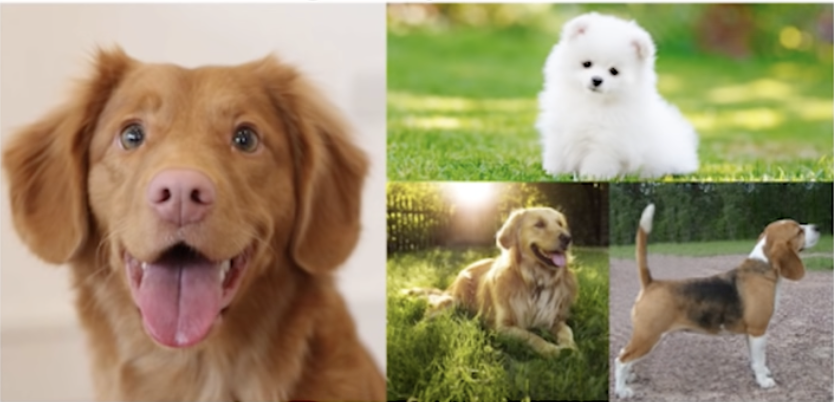
\includegraphics[width=\textwidth]{figures/intro/dogs_train.png}
         \caption{Dogs train set.}
     \end{subfigure}
     \hfill
     \begin{subfigure}[b]{0.49\textwidth}
         \centering
         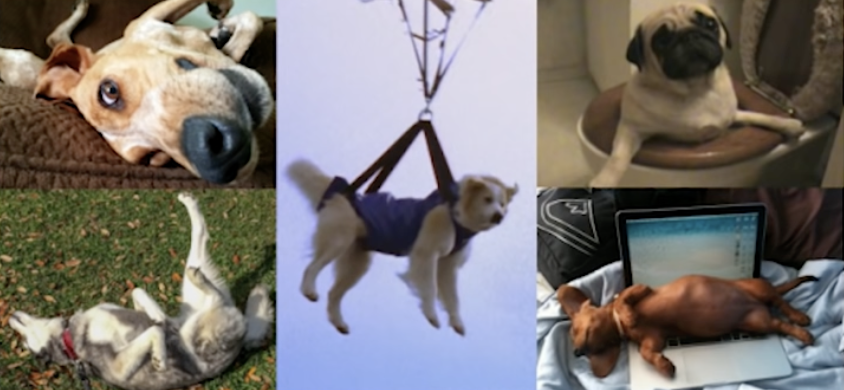
\includegraphics[width=\textwidth]{figures/intro/dogs_test.png}
         \caption{Dogs test set.}
     \end{subfigure}

     \hfill
     \begin{subfigure}[b]{0.49\textwidth}
         \centering
         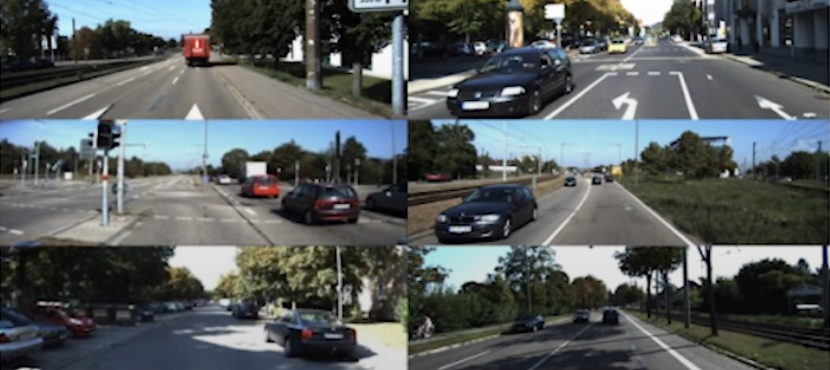
\includegraphics[width=\textwidth]{figures/intro/cars_train.png}
         \caption{Cars train set.}
     \end{subfigure}
     \hfill
     \begin{subfigure}[b]{0.49\textwidth}
         \centering
         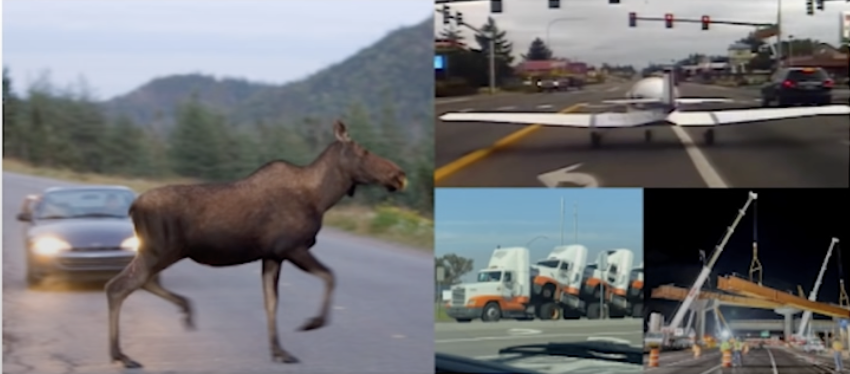
\includegraphics[width=\textwidth]{figures/intro/cars_test.png}
         \caption{Cars test set.}
     \end{subfigure}
     \caption{Discrepancies between training and testing 
     distributions (\href{http://introtodeeplearning.com/2021/slides/6S191_MIT_DeepLearning_L7.pdf}{source}).}
     \label{fig:discrepancies-train-test-distributions}
\end{figure}

\section{Objectives}

The purpose of this thesis is twofold:
\begin{enumerate}
    \item On the one hand, to build a Python package that offers a standardised \textit{scikit-learn} compatible API to train and evaluate uncertainty quantification models. This package shall be able to transform any classification or regression model following a \textit{scikit-learn} API into an updated model capable of evaluating its uncertainty.
    \item On the other hand, to provide insights into the occurrence of hallucinations in the current graph-to-text pipeline at Oracle and how they can be related to uncertainty. The following research questions shall be answered:
    \begin{enumerate}
        \item What are the different approaches to estimating uncertainty in text generation and/or sequence-to-sequence models? How do these approaches compare in terms of performance?
        \item What is the relationship between uncertainty and hallucination? To what extent is it possible to use uncertainty quantification to detect hallucinations?
    \end{enumerate}

\end{enumerate}

\section{Problem statement} \label{intro:problem-section}

%\subsubsection{The uncertainty function}

As discussed in the previous sections, understanding how much evidence the model has in its predictions can be equally as important as the predictions themselves. The quantification of uncertainty can be formalised as follows. Let $D_{train}=\{x_i\}_{i=1}^N$ be the training dataset where each data point is $D$ dimensional and let $\hat y_i = f(x_i)$ be the models predictions. The goal of UQ is to produce scores 
$u_i = U_f(x_i)$
such that $u_i$ is high when the model error is high and conversely. The usual candidates for the uncertainty function $U$ are the standard deviation (respectively the entropy) of the prediction distribution in the regression (respectively classification) case.   
Furthermore, two scenarios can occur during the evaluation on a testing data set $D_{test}$, which may not follow the same underlying distribution as $D_{train}$, i.e. out of distribution data points. On the one hand, the model may perform similarly on $D_{test}$ compared to $D_{train}$, which indicates a low generalisation error. In this case, the uncertainty should be roughly comparable between the two datasets. On the other hand, the model may under-perform on $D_{test}$ and the following property is expected to hold

\begin{equation}
    \E_{p(X \mid D_{test})} [U_f(X)] \geq  \E_{p(X \mid D_{train})} [U_f(X)] 
\end{equation}

If not, it implies that the model is more confident over incorrect predictions, which is a failure for $U$ to capture the inherent uncertainty of the model.
If this definition covers most classification use cases, it needs to be slightly adapted for text generation. Indeed, the output of the model is composed of multiple tokens 
$
\hat y_i = [t_{i,1}, \ldots, t_{i,L}]
$
and it is natural to define the uncertainty function at the same token granularity
$
u_i = [u_{i,1}, \ldots, u_{i,L}]
$.
Nevertheless, for readability purposes, these scores could be aggregated into decoded words, sentences, etc.

\section{Illustrative examples}

This section contains visual interpretations of the output of UQ models for a regression and a text generation use case.
For the first case, UQ usually consists of confidence intervals or standard deviations. In figure \ref{fig:uq-regression-example}, three different UQ model predictions are displayed for the same underlying mean prediction function. Ultimately, the objective of UQ models is to reach the performance of the third model (cf. figure \ref{uq-regression-example-calibrated}) so that it is neither over nor under-confident and these uncertainty scores can be trusted by the model's user. 

\begin{figure}
     \centering
     \begin{subfigure}[b]{0.32\textwidth}
         \centering
         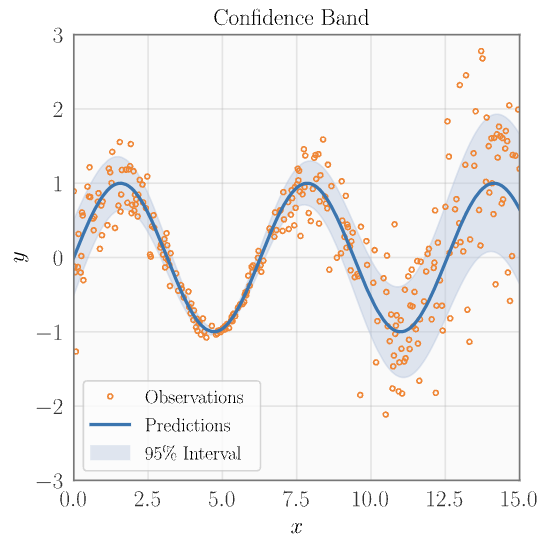
\includegraphics[width=\textwidth]{figures/intro/example-under.png}
         \caption{Over-confident UQ model.}
        % \label{fig:y equals x}
     \end{subfigure}
     \hfill
     \begin{subfigure}[b]{0.32\textwidth}
         \centering
         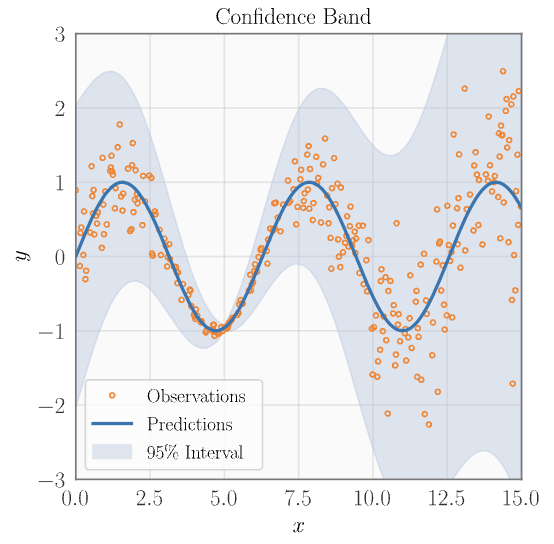
\includegraphics[width=\textwidth]{figures/intro/example-over.png}
         \caption{Under-confident UQ model.}
       %  \label{fig:three sin x}
     \end{subfigure}
     \hfill
     \begin{subfigure}[b]{0.32\textwidth}
         \centering
         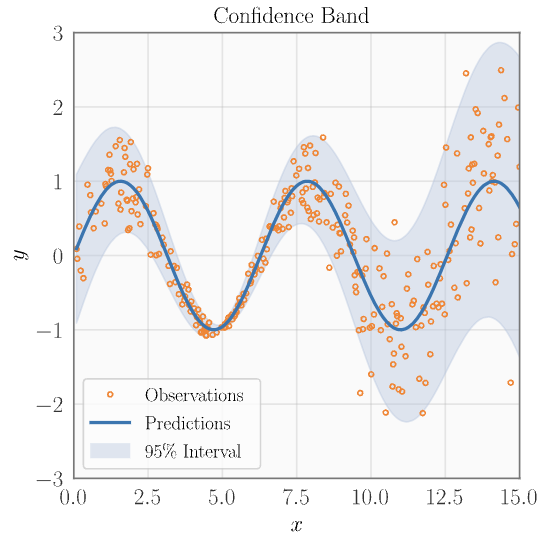
\includegraphics[width=\textwidth]{figures/intro/example-good.png}
         \caption{Calibrated UQ model.}
         \label{uq-regression-example-calibrated}
     \end{subfigure}
        \caption{Examples of uncertainty quantification models for regression (\href{https://github.com/uncertainty-toolbox/uncertainty-toolbox}{source}).}
        \label{fig:uq-regression-example}
\end{figure}

% Example: forecasting model of the return of a portfolio over time. 

When it comes to text generation, one particular text instance of the WebNLG dataset is considered, as well as the following model response, in an attempt to reproduce this text.

\epigraph{Alan Bean was an American astronaut, born on March 15, 1932, in Wheeler, Texas. He received a Bachelor of Science degree at the University of Texas at Austin in 1955 and was chosen by NASA in 1963.}{Reference text}

\epigraph{
Alan Bean was an American astronaut, born on March 15, \textbf{1948}, in Wheeler, Texas. He received a Bachelor of Science degree at the \textbf{Massachusetts Institute of Technology} in 1955 and was selected by NASA in 1963.
}{Model prediction}

The model has introduced some errors for the birth year as well as the name of the college university. A valid uncertainty quantification model should produce an output similar to the following. Note that uncertainty scores appear on top of the text with the convention that higher red intensity corresponds to a higher uncertainty score.

\epigraph{
Alan Bean was an American astronaut, born on \textcolor{Salmon}{\textbf{March}} 15, \textcolor{BrickRed}{\textbf{1948}} in Wheeler, Texas. He \textcolor{Salmon}{\textbf{received a}} Bachelor of Science degree at the \textcolor{BrickRed}{\textbf{Massachusetts Institute}}  \textcolor{Salmon}{\textbf{ of Technology}} in 1955 and was \textcolor{Salmon}{\textbf{selected}} by NASA in 1963.
}{Model prediction with uncertainty}





%%%%%%%%%%%%%%%%%%%%
\chapter{Background}  \label{chatper:background}
%%%%%%%%%%%%%%%%%%%%
%The background section introduces the necessary background to understand your work. This is not necessarily related work but technologies and dependencies that must be resolved to understand your design and implementation. 

%This section is usually 3-5 pages.


\section{Uncertainty decomposition}
% Uncertainty in ML - difference data/model uq

The uncertainty in ML can be decomposed into two components\cite{surveyUQinDL} (cf. figure \ref{fig:data-mode-uncertainty-illustration}). 
On the one hand, the data (or aleatoric) uncertainty describes the confidence in the data. It is highest when the data is noisy, e.g. in class overlap situations. While it is independent of the number of data points, it can be reduced by revising the data-gathering process, e.g. adding features or selecting more accurate sensors.
On the other hand,  model (or epistemic) uncertainty reflects the model's confidence in the prediction. Model uncertainty can be used to figure out when the model cannot provide a reliable answer or when it is missing some training data to provide that answer. Unlike data uncertainty, model uncertainty can be reduced by adding more data and thus improving the model's confidence. It is considerably more challenging to estimate than data uncertainty.

% $$\E_{p(\theta \mid D)} [U(]$$


% add figures

\begin{figure}
     \centering
     \begin{subfigure}[b]{0.49\textwidth}
         \centering
         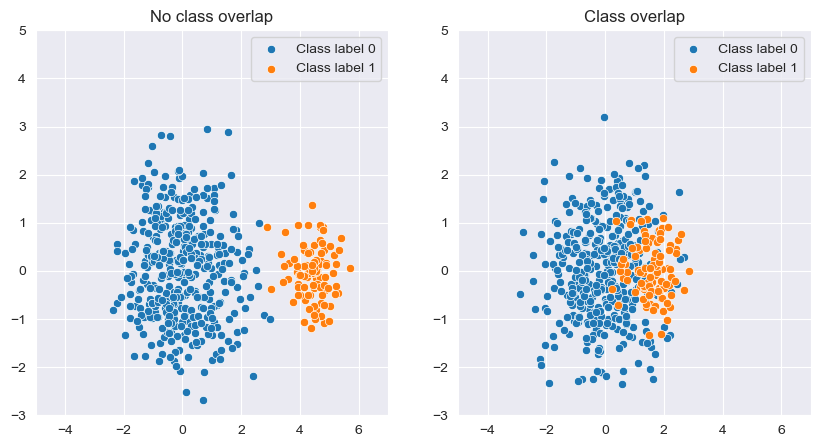
\includegraphics[width=\textwidth, height=140pt]{figures/related_work/classoverlap.png}
         \caption{Data uncertainty is higher when class overlap is present.}
     \end{subfigure}
     \hfill
     \begin{subfigure}[b]{0.49\textwidth}
         \centering
         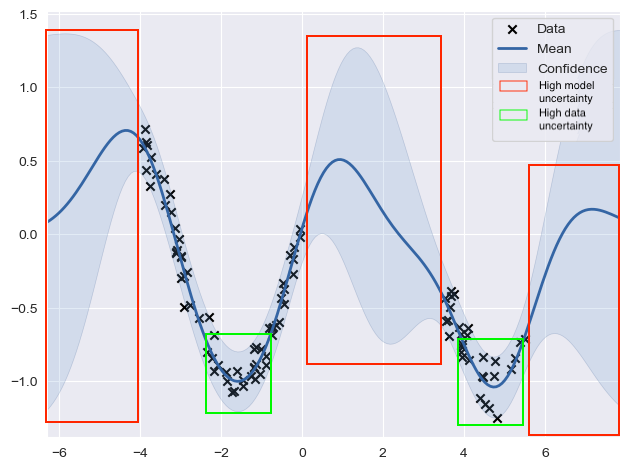
\includegraphics[width=\textwidth,height=140pt]{figures/related_work/gp.png}
         \caption{Difference between data and model uncertainty.}
     \end{subfigure}
     \caption{Data and model uncertainty.}
     \label{fig:data-mode-uncertainty-illustration}
\end{figure}

% explain UQ decomposition using heart-shaped data



Furthermore, in a text-generation application, the data uncertainty can be further divided into the following categories:
\begin{enumerate}
    \item Language uncertainty: the uncertainty of the language model itself, e.g. multiple different formulations can be used to express the same idea.
    \item Factual uncertainty: the uncertainty of the factual knowledge, e.g. in a question-answering use case, the model could answer incorrectly or even fabricate unrealistic answers, i.e. hallucinations.
    \item Input uncertainty: the uncertainty of the input data (prompt, context, etc.), e.g. the input could be noisy or contain errors. This is especially relevant for sequence-to-sequence or data-to-text models.
\end{enumerate}

\section{Calibration}

Machine learning models don't always produce reliable uncertainty estimates, e.g. classifiers are often over or under-confident regarding the SoftMax output probabilities. In addition, $\alpha$-confidence intervals might not cover the true value with an $\alpha$ probability.  % produced under wrong assumptions (e.g. normality, homoscedasticity, etc.)  
Poorly calibrated predictions negatively impact users who make informed decisions based on these predictions, especially in sensitive domain applications like healthcare. % talk about probability threshold. 
Model calibration is a post-training technique to adjust the predicted probabilities of a model so that they accurately reflect the true underlying probabilities of the events being predicted. True probabilities are estimated empirically using an extra dataset that is called the calibration dataset. Platt scaling\cite{platscaling}, Isotonic regression\cite{isotonicRegression}, and temperature scaling are common practical implementations of calibration. 

Calibration is often visualised using reliability diagrams (cf. figure \ref{fig:calibration-example}). In a binary classification task, the predicted probabilities of the true class are compared against the empirical class membership probabilities computed using the calibration dataset. Any deviation from the diagonal line is considered to be a calibration failure. Based on these plots, the area between the diagonal and the reliability curve is often used as a metric to assess the quality of an uncertainty quantification model.
%$P(c | score(x) = s)$
\begin{figure}
    \centering
    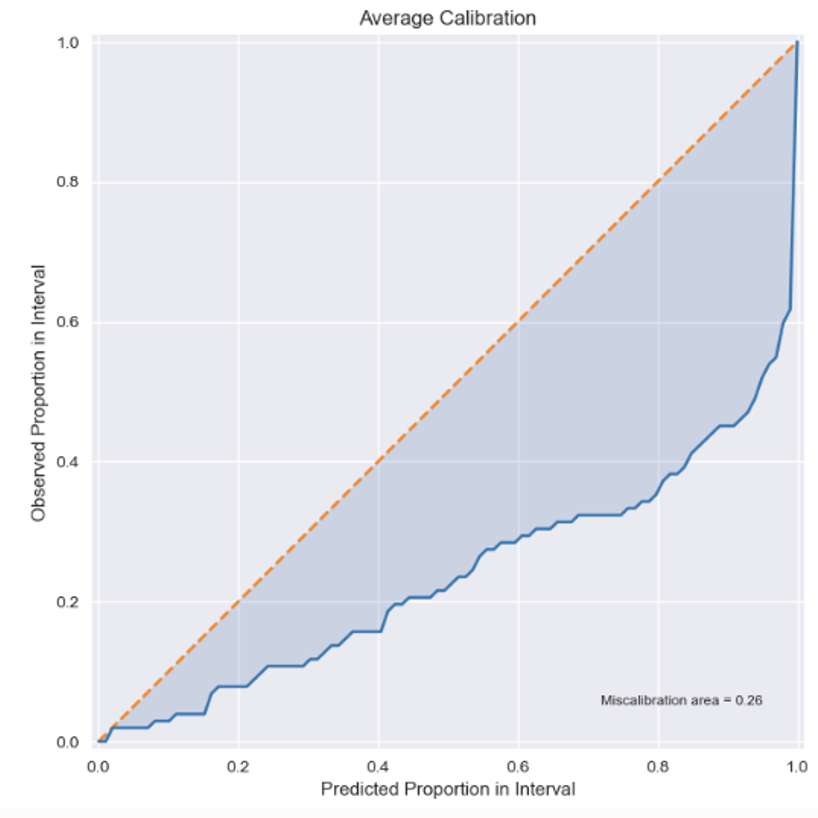
\includegraphics[scale=0.58]{figures/related_work/calibration.png}
    \caption{Example of reliability diagram for an under-confident model. The orange line represents a perfectly calibrated model. The data point (0.6,0.3) can be interpreted as follows: when the model predicts a 60\% probability of belonging to the true class, there is empirical evidence of 30\% in the calibration dataset that the prediction is a true positive.}
    \label{fig:calibration-example}
\end{figure}

Platt scaling is one of the most popular calibration methods and was initially introduced for support vector machine models. Consider a binary classification use case: given uncalibrated prediction probabilities for the true class label $\{ p_i \}_{i=1}^N$, Platt scaling optimises a parametric model based on the logistic function defined by
$$
f(p_i \mid A, B) = \Pb( y = 1 \mid p_i) = \frac{1}{1 + e^{- (A \cdot p_i + B)}}
$$
After training both parameters $A > 0$ and $B > 0$, the corrected probabilities are $\Tilde p_i = f(p_i)$.

In contrast, isotonic regression is a non-parametric regression over the class of non-decreasing (i.e. isotonic) functions, i.e. $\forall_{i,j}$ if $ p_i \leq p_j$ then $\Tilde p_i \leq \Tilde p_j$. The Pair-adjacent violators (PAV) algorithm is commonly used to fit an isotonic stepwise-constant function $I$ by optimising the mean-square error criterion. The isotonic property of the mapping function enforces the same probability ranking before and after applying the function. Due to its non-parameter nature, it usually requires more training data than Platt scaling and is more prone to overfitting.

Finally, temperature scaling (TS) is a single-parameter variation of the Platt Scaling approach. It rescales logit scores by a parameter $T$ before applying the SoftMax function $SoftMax(f_i / T) $ to better match the empirical class membership probabilities. TS is straightforward yet effective while maintaining a low memory complexity to calibrate machine learning models, also in the case of deep neural networks\cite{TSDeepNets}.

% (a) show calibration picture.


\section{Bayesian learning}

Bayesian learning takes a different approach than traditional frequentist machine learning to perform statistical inference by modelling a complete distribution over possible parameters of the model instead of point estimates. At its core, Bayes' theorem allows the incorporation of prior information about the model parameters into the prediction process. Let $D_{train} = \{X,Y\}= \{(x_i,y_i)\}_{i=1}^N$ be the training set so that $x_i \in \R^D$ and $y_i \in \R$ or $y_i \in \{1,\ldots,C\}$ depending on whether the application is a regression or a classification. Bayesian learning aims to optimise the weights $\theta$ of the model $f_\theta(\cdot)$ using the posterior distribution 
$$
\Pb(\theta \mid X, Y) 
= \frac{\Pb(Y \mid X, \theta) \cdot \Pb(\theta) }{\Pb(Y \mid X) }
\propto Likelihood \, \times \, Prior
$$

The complexity of this operation depends on the marginalisation step, which cannot be computed analytically in most real-life scenarios:
$
\Pb(Y \mid X) = \int \Pb(y \mid x, \theta) \cdot \Pb(\theta \mid X,Y) \;d\theta
$.


To address this issue, variational approaches propose to approximate $\Pb(\theta \mid X, Y)$ using variational parameters $q_\omega(\theta)$ so that the Kullback–Leibler divergence between both distributions, $KL(q_\omega(\theta) \parallel \Pb(\theta \mid X, Y) )$, is minimised with respect to $\omega$. 
The Bayesian counterpart of neural networks, Bayesian Deep Learning (BDL) and Bayesian NNs (BNNs), are popular methods to interpret the model parameters and produce insights about their reliability without overfitting the data. Tools such as Monte Carlo (MC) dropout\cite{dropoutDeepNets}, Markov chain Monte Carlo (MCMC) or Variational inference (VI) are used to approximate the posterior inference. Multiple estimates for the target variable can be produced via a sampling procedure over the weight distribution, which can be turned into an uncertainty score.
 

\section{Ensembles} \label{section:background:ensembles}

Ensemble learning is a machine learning tool that trains multiple different predictors and combines their results into a final prediction. Ensembles aim to reduce the model's variance and produce more accurate and robust predictions than any of the underlying predictors, which can be prone to over-fitting or under-fitting the training data. 
One of the most popular methods to combine these predictions is to take their simple average. However, other methods exist, such as taking the median or the weighted average, which puts more influence on specific models.
Ensembling is a very popular technique used in a wide range of applications. Many popular algorithms, such as Random Forests, are based on this principle. They also have major implications in the uncertainty quantification field, as shown in section \ref{model:uq-ensembles}.



% other question how to create the ensemble?
% discrete and finite set of learners => if infinite => tend to bayesian learning.
% variance reduction => improve bias-variance tradeoff
% In the literature, ensembles are often used to predict the mean and not variance

\section{Adversarial machine learning}

Along with the widespread of machine learning in day-to-day use, such as medical applications or self-driving cars, there has also been a growing concern for security and robustness in these systems. Interestingly, it turns out that many of the top-performing models are vulnerable to what are called adversarial examples. These are crafted inputs which may be indistinguishable from original inputs to human eyes and yet have been specifically designed to cause a failure for the model to classify them correctly.
Therefore, adversarial machine learning aims to deceive or mislead the model or person relying on its predictions using attacks and to learn how to defend against them. 

%%%%%%%%%% survey paper on adversarial ML
Nowadays, various threat models and adversaries can be exploited by attackers to attempt to break these models. Still, only a limited number of countermeasures are available to act against them. Defence is articulated around two pillars: attack detection to filter them before they enter the system and special training to make models more robust against them. On the attack side, adversarial examples can be generated, for instance, using optimisation-based methods. One widely known attack is the fast gradient sign method (FGSM)\cite{FGSM} that leverages the gradient of the loss function with respect to the input data to create small perturbations that are then turned into adversarial examples. This attack is fast and powerful since it can be computed efficiently using back-propagation in the case of neural networks.

\section{Knowledge Graphs}
\say{
A knowledge graph mainly describes real-world entities and their interrelations, organised
in a graph\cite{KnowledgeGraphDef}.}. Even though more formal definitions have been proposed\cite{KnowledgeGraphDefFormal}, this simple definition covers the needs of this work. Knowledge graphs are often represented in the Resource Description Format (RDF), i.e. into a set of triplets. Triples encode edges of the graph in a subject-predicate-object format such as \textit{(John, is friend with, Bob)}. 

% Idea: DBPedia dataset 

\section{Natural Language Processing}

Natural Language Processing (NLP) focuses on the relationship between human language and computer systems. It is an interdisciplinary domain at the intersection of linguistics, computer science and artificial intelligence. In particular, NLP aims to build algorithms capable of understanding and extracting pieces of information from a text corpus or generating human-like texts. The latter tasks are the concentration area of this thesis regarding NLP. The following sections introduce the necessary concepts to understand chapter~\ref{chatper:design}.

\subsection{Named-Entity Recognition}

Named-Entity Recognition (NER) is the process of identifying and classifying entities in unstructured texts. Usually, a fixed set of entities are considered, e.g. organisations, person names, time and dates, quantities, etc. An example of NER output is shown below (\href{https://tdai.osu.edu/sites/default/files/2022-06/2022-foundations-tutorial3-sunwang-deeplearning4nlp.pdf}{source}):

\begin{center}
    Ousted [WeWork]\textsubscript{Organisation} founder [Adam Neumann]\textsubscript{Person} lists his [Manhattan]\textsubscript{Location} penthouse for [\$37.5 million]\textsubscript{Amount}.
\end{center}

First, different entities can be identified, i.e. localised in the text: \textit{WeWork}, \textit{Adam Neumann}, \textit{Manhattan} and \textit{\$37.5 million}. Then, they can be classified further into the following categories: \textit{organisation}, \textit{person}, \textit{location} and \textit{amount}. This two-step procedure is a common abstraction of the NER task. However, many practical implementations, such as the state-of-the-art transformed-based models, do not follow this structure. More formally, each named entity $NE_i$ in a text $T = \{t_1,\ldots,t_n\}$ composed of $n$ tokens is defined by a triple $NE_i= (s_i, e_i, c_i)$ where $s_i, t_i \in \{1, \ldots, n\}$ respectively represent the start and end index of the entity in the text. $c_i$ corresponds to one of the predefined entity types. %discuss evaluation if needed.

\subsection{Transformers}

Transformers are a type of neural network architecture introduced in 2017\cite{transformers} based on the concept of self-attention to construct contextualised word embeddings. 
Transformers have grown in popularity ever since and now serve as a reference point for many NLP tasks such as machine translation, text classification or language generation. One of the key benefits of this architecture is its ability to process larger amounts of text efficiently and better exploit long-range dependencies in the input text compared to other models such as RNNs or LSTMs. 
% explain how pretraining-fine tuning works
These models have also popularised the concept of transfer learning, i.e. pre-training and fine-tuning. In the first phase, they are trained using a self-supervised procedure on a large corpus of unannotated text usually taken from the Web. The training task differs from one model to another, but the most simple one is to predict the next work in a sequence given the previous ones and is known as language modelling. BERT\cite{BERT} uses a slight variation called masked-language modelling (MLM) that predicts masked words:

\epigraph{
The boy walked to the store, but he realised he forgot his \textbf{[MASK]} on the kitchen table.
}{Example of a masked language modelling input}
\newpage
In the second fine-tuning phase, the model is adapted to a downstream task using a considerably smaller dataset than the pre-training corpus. Fine-tuning is about harvesting the language information stored during pre-training and slightly updating the weights better to match the vocabulary and style of the downstream task.   
% focus on transformer architecture
The original transformer used an encoder-decoder architecture. The input is processed by a series of encoding layers that extract information about which parts of the input are relevant to the others. The decoder takes a reversed approach and starts from the contextualised word representations created by the encoder to reconstruct a sequence of tokens as output. Both components operate using an attention mechanism that can be decomposed into scaled dot-product attention units. Each unit learns three weight matrices to  produce embeddings for every token:  the query weights $W_{Q}$, the key weights $W_{K}$, and the value weights  $W_{V}$. Given $X$, the matrix containing word embeddings as rows, $Q = X \cdot W_Q$, $K = X \cdot W_K$ and $V = X \cdot W_V$, the attention scores $A$ can be computed as follows

$$
A = Softmax \left(\frac{Q \cdot K^T}{\sqrt{d_k}} \right) V
$$
where $\sqrt{d_k}$ is a gradient stabilisation factor during training. 

% to be paraphrased 
% The final word embedding not only contain information about the word itself but also a combination of other tokens, each weighted by its attention weight

At inference time, transformers rely on decoding algorithms to produce human-like text. The most straightforward one is greedy decoding which is fast but tends to deliver redundant and dull outputs\cite{issuesDecodingSamplingNLP}. At each step, the highest probability token given the previously generated ones is selected. This causal procedure is repeated until some desired length is reached or an end-of-sequence token is generated. Beam search decoding has been proposed to offer more diverse and probable sequences. It maintains a buffer of the $B$ most probable sequences generated so far, i.e. the beams. At each step, each of these beams explores the next $B$ most probable tokens which result in $B^2$ possible candidates. Those with the lowest joint probability are pruned so that only the top $B$ candidates remain. As the beam size $B$ increases, beam search becomes slower to execute with a lower bound at $B=1$, i.e. greedy search. Alternatively, stochastic text generation approaches utilise the token probability distribution to sample the tokens at each step to avoid generic outputs. Random sampling is a simple strategy but tends to produce several rare tokens and, thus, unrealistic text. To address this issue, different sampling variations have been introduced to cut-off probability mass for unlikely tokens. Top-K sampling exclusively considers the K most probable tokens. In contrast, nucleus sampling\cite{nucleusSampling} is based  on Top-$L$ sampling where $L$ is the smallest integer so that the cumulative probability distribution for these $L$ tokens exceeds some probability threshold $p$.



% conclusion before next section
Part of their success can also be attributed to the open-source access of pre-trained implementations, e.g. the BERT-family of models created by HuggingFace. In this thesis, specific focus has been directed to the text-to-text transfer transformer or T5\cite{T5}.

\subsection{T5 and sequence-to-sequence models}

Sequence-to-sequence models are based on the encoder-decoder architecture and are used to transform one sequence into another where input and output can be of arbitrary length. The goal of the encoder is to create a fixed-length numeral representation of the input sequence, %, i.e. the last hidden state, 
which is then passed to the decoder. The decoder leverages this information as part of the auto-regressive output sequence generation to produce input-dependant tokens.

T5 or the text-to-text transfer transformer\cite{T5} is an example of the sequence-to-sequence architecture. As opposed to the BERT-family of models that can only return a class label or a span of the input,  T5 is, at its essence, a standardised proposal to represent all NLP tasks in a text-to-text format. In other words, the same model, loss function and hyper-parameters are used to simultaneously train heterogeneous tasks such as machine translation, question answering, sentiment analysis, etc. The pre-training objective of T5, i.e. sized-fill-in-the-blank text generation, differs from BERT's MLM because the model is asked to fill an approximate number of words at some specific place in the sentence, which can also be at the end. For example, given as input the string \textit{"I like to eat peanut butter and \_4\_ sandwiches"}\cite{googleBlogT5}. The model could fill the blank using the sequence: \textit{"jelly, which is what makes good"} while a size-2 masked token \textit{\_2\_} would result in \textit{"jelly on my"}.



% T5 pre-training task from google
% https://ai.googleblog.com/2020/02/exploring-transfer-learning-with-t5.html


\subsection{Graph-to-text and text-to-graph} \label{background:G2T}

% data2text models are prone to hallucinations compared to template-based models\cite{challengesData2Text}


% into what is a graph to text and goals
The graph-to-text generation task aims to convert structured information given as a graph into a fluent textual output. On the other end, text-to-graph is the converse task of extracting relevant entities from the input text, i.e. nodes, and the relationships between them, i.e. edges. Graph-to-text models can be used for a variety of tasks, including question-answering, content generation, etc. In contrast, text-to-graph models are more applicable to data-mining or information extraction.
%different pipeline approach
Consider an example from the WebNLG dataset: the graph is shown in table \ref{table:example:graph}, and the reference text is:

\epigraph{
Alan Bean was an American astronaut, born on March 15, 1932, in Wheeler, Texas. He received a Bachelor of Science degree at the University of Texas at Austin in 1955 and was chosen by NASA in 1963.
}{Reference text}

\begin{table}[ht]
\centering
\caption{Graph example from WebNLG dataset in RDF format.}
\label{table:example:graph}
\begin{tabular}[t]{llll} % p{3cm}
\hline
 &  Subject & Relation & Object \\
\hline
1& Alan Bean & nationality & United States \\
2& Alan Bean & birth date   & 1932-03-15    \\
3& Alan Bean & alma mater   & UT Austin, B.S. 1955 \\
4& Alan Bean & birth place  & Wheeler, Texas \\
5& Alan Bean & selection   & 1963 \\
\hline
\end{tabular}
\end{table}%



% currently 

As of today, state-of-the-art models are built using sequence-to-sequence transformers such as T5. As a result, the graph must first go through a linearisation process to be transformed into a sequential textual representation that can then be fed to the model for training. Special tokens $<H>$, $<R>$ and $<T>$ are added to the tokenizer of the model to put emphasis respectively on the start of the subject, relation and object part of each edge. After concatenating all edges one after the other, the linearised example graph becomes:

\epigraph{
<H> Alan Bean <R> nationality <T> United States
<H> Alan Bean <R> birth date <T> 1932-03-15
<H> Alan Bean <R> alma mater <T> UT Austin, B.S. 1955 
<H> Alan Bean <R> birth place <T> Wheeler, Texas
<H> Alan Bean <R> selection <T> 1963
}{linearised graph}

% explain 
The linearised graph and text pairs are then used to fine-tune two independent T5 models, one for graph-to-text and one for text-to-graph. Even though this approach generates highly performing models, the linearisation phase has been criticised in the literature due to its inability to exploit the structural properties of the graph. Models such as JointGT\cite{JointGT} have been proposed to improve the encoding phase of the transformer. However, they are not considered in this thesis work. 

%In addition, manual data collection and labelling is often a tedious process for these models, resulting in scarce training datasets. To overcome this issue, an unsupervised approach, CycleGT\cite{cycleGT}, was introduced in 2020. It trains both graph-to-text and text-to-graph pipelines in rounds with unpaired text and graph datasets. It has been shown to reach comparable performance to supervised counterparts.





%%%%%%%%%%%%%%%%%%%%%%
\chapter{Related Work}  \label{chatper:related-work}
%%%%%%%%%%%%%%%%%%%%%%

%The related work section covers closely related work. Here you can highlight
%the related work, how it solved the problem, and why it solved a different
%problem. Do not play down the importance of related work; all of these
%systems have been published and evaluated! Say what is different and how
%you overcome some of the weaknesses of related work by discussing the 
%trade-offs. Stay positive!

%This section is usually 3-5 pages.

%%%%%%%%%%%%%%%%%%%%%%%%%%%%%%%%%%%%

\section{Uncertainty quantification models}

\subsection{Probabilistic learning} \label{model:probabilistic-learning}

In a classical supervised learning problem, let $D_{train} = \{(x_i, y_i)\}_{i=1}^N$ be the training set and $y_i$ can be either discrete or continuous. The objective of the machine learning model is often phrased as follows: given $D_{train}$, learn a prediction function $f$ from input variable $X$ to the target variable $y$ such that $f(X) = \EX[y \mid X]$. In other words, supervised learning is about predicting a point estimate, i.e. the expectation of the target distribution given the input. However, the expectation only contains limited information about the target distribution, and it is unable to reflect any form of uncertainty about that distribution. Probabilistic learning methods propose to address this issue, for instance, by also modelling the variance or spread of the target distribution $Var[y \mid X]$. For the case of classification, modelling a full probability distribution over discrete classes is already part of the underlying prediction mechanism, i.e.  $y = \argmax_k \; \Pb[y = k \mid X]$. In this case, the entropy of the prediction distribution is considered to be a valid measure of uncertainty.

For the regression case, the usual assumption is to consider a normally distributed target variable with mean $\mu$ and standard deviation $\sigma$, i.e. $y \sim \Normal(\mu, \sigma^2)$ and optimise the following negative log-likelihood loss to learn a model to return both the mean and standard deviation:

$$\Loss(\mu, \sigma)  = \frac{1}{2N} \sum_i \log \sigma_i^2 + \left ( \frac{y_i - \mu_i}{\sigma_i}\right)^2$$
 
The different properties of probabilistic learning methods are summarised in table \ref{table:probabilistic-learning}. As a final note, it is essential to realise that uncertainty scores produced by this approach only take into consideration the data uncertainty component. 




\begin{table}[ht]
\centering
\caption{Probabilistic likelihood estimation.}
\label{table:probabilistic-learning}
\begin{tabular}[t]{lcc} % p{3cm}
\hline
&Classification (discrete) & Regression (continuous)\\
\hline
Targets     & $y \in \{1,\ldots, K\}$   & $y \in \R$  \\
Likelihood  & $y \in Categorical$       & $y \sim \Normal(\mu, \sigma^2)$\\
Parameters  & $p=\{p_1, \ldots, p_K\}$    & $(\mu, \sigma)$\\ 
Constraints  & $\sum_k p_k = 1$          & $\mu \in \R$; $\sigma > 0$\\
Loss function & $-\sum_k y_k \log p_k$  & $ - \log  \Normal(y \mid \mu, \sigma^2)$\\
Uncertainty measure & $\Entropy(p)$ & $\sigma$ \\
\hline
\end{tabular}
\end{table}%




\subsection{Quantile regression} \label{model:quantile-regression}

Quantile regression\cite{quantileRegression} is a statistical tool that extends the least squares algorithm to model the conditional $\alpha$ quantile of a target distribution instead of the conditional mean. % a % given certain predictor variables. 
These models optimise an asymmetrically weighted sum of absolute errors loss function:

$$
\Loss(\theta) =\frac{1}{N} \sum_i 
\begin{cases}
    \alpha \cdot (y_i - x_i^T  \theta), \;\;\; y_i \geq x_i^T  \theta \\
    1-\alpha \cdot (x_i^T  \theta - y_i),\;\;\; y_i < x_i^T  \theta \\
\end{cases}
$$

which penalises data points if the $\alpha$ quantile is low (respectively high), but the predicted quantile is high (respectively low). Quantile regression is an effective tool to produce uncertainty scores and, in particular, confidence intervals. Given a tolerance $\tau$, two extra models are trained, i.e. $f_{low}$ with parameter $\alpha_{low} = \frac{\tau}{2}$ for the lower confidence bound and $f_{high}$ with parameter $\alpha_{high} = 1-\frac{\tau}{2}$ for the upper bound so that $\Pb[ f_{low}(X) \leq Y \leq f_{high}(X)] \leq 1-\tau$. Quantile regression can capture asymmetrical relationships between the target and input variables. An example of a quantile regression model is shared in figure \ref{fig:quantile-regression}.



\begin{figure}[!ht]
    \centering
    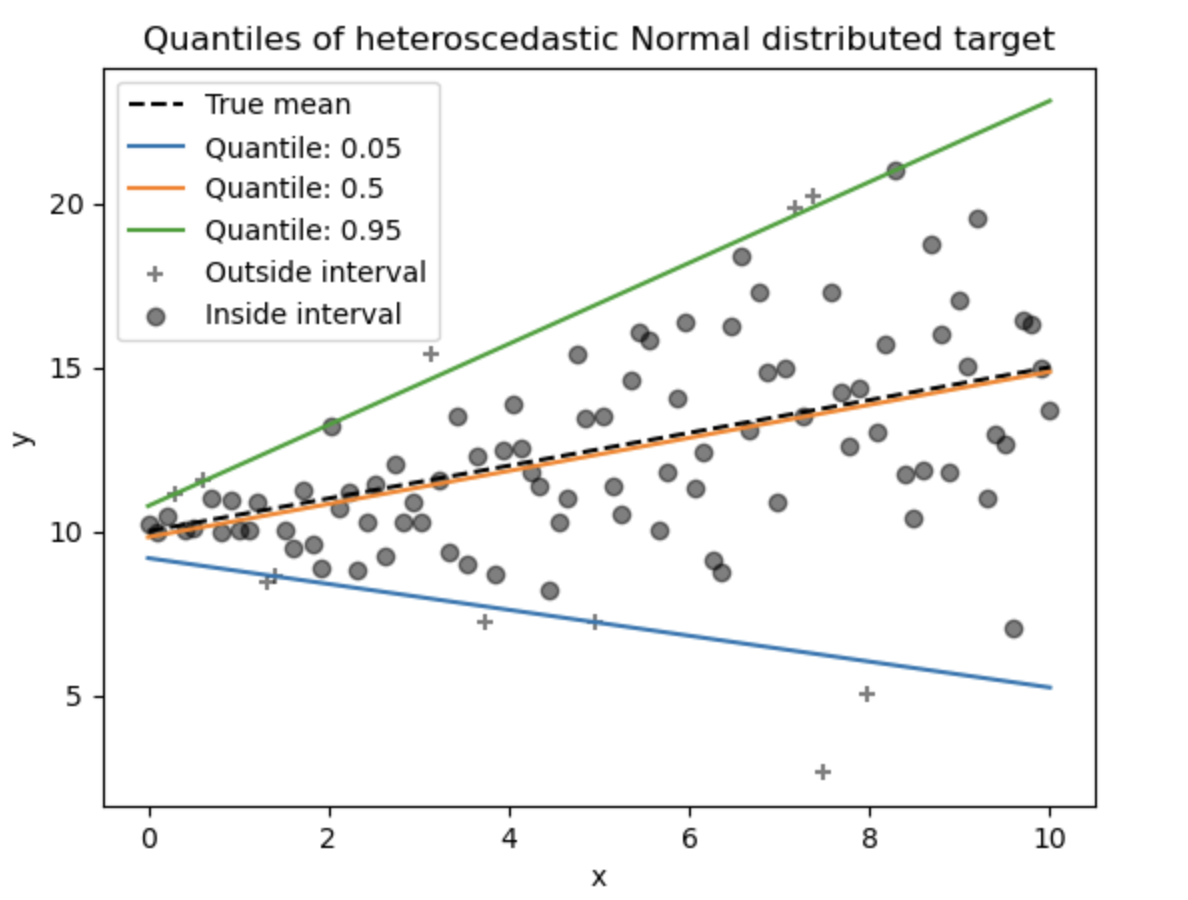
\includegraphics[scale=0.45]{figures/related_work/quantile_regression.png}
    \caption{Example of quantile regression for $\alpha = 0.05$, $0.5$ and $0.95$ (\href{https://scikit-learn.org/stable/auto_examples/linear_model/plot_quantile_regression.html}{source}).}
    \label{fig:quantile-regression}
\end{figure}


\subsection{Conformal prediction} \label{model:conformal-prediction}

Conformal prediction\cite{conformalPredictions2021} is an uncertainty quantification tool for classification models that proposes to predict multiple plausible target values instead of a single one. The output of conformal prediction is called prediction sets (cf. figure \ref{fig:conformal-prediction-example}). Prediction sets $C(x_{test}) \subset \{1,\ldots, |V|\}$ are guaranteed to contain the ground truth with a user-specified probability $\alpha$

$$
1 - \alpha \leq P(Y_{test} \in C(x_{test})) \leq 1 - \alpha + \frac{1}{n+1}
$$

The statistical guarantee provided by conformal prediction is similar to confidence intervals in the regression case and can be understood as a form of calibration. Additionally, this approach is versatile and applicable to black-box settings as it is model agnostic and distribution-free. Any trained classification model can be transformed into a conformal prediction model with the acquisition of a few additional data points (i.e. calibration dataset) for the calibration process.

\begin{figure}
    \centering
    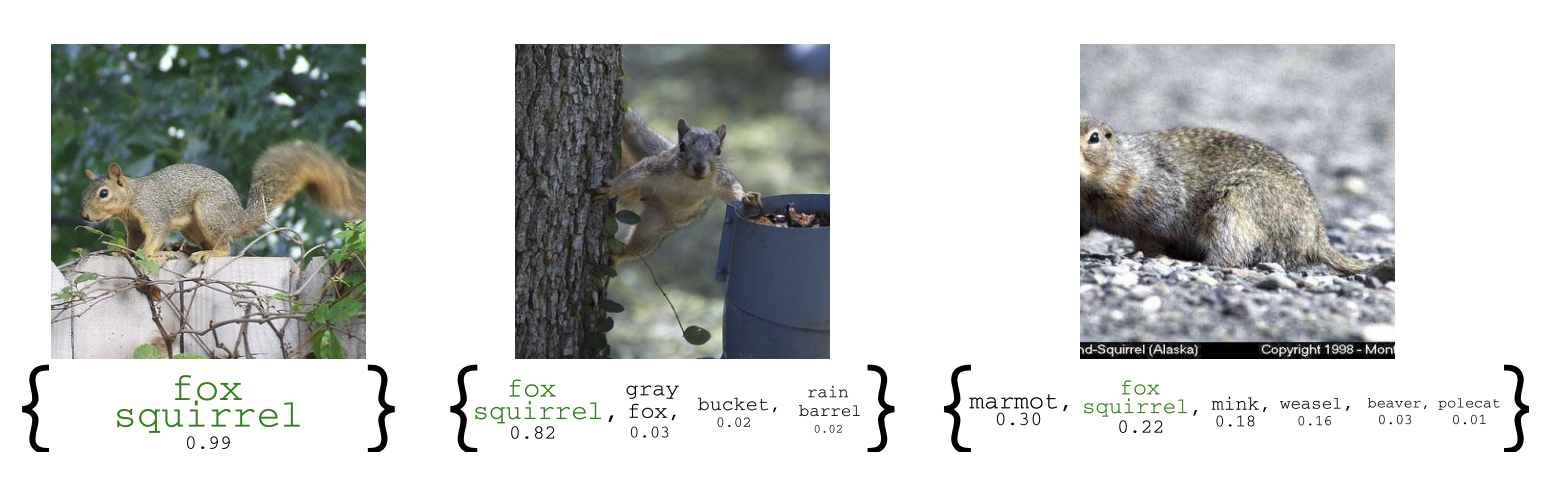
\includegraphics[scale=0.55]{figures/related_work/conformal_predictions.png}
    \caption{Conformal prediction. ImageNet's prediction set examples from\cite{conformalPredictions2021}. More complex examples involving fox squirrel prediction are shown from left to right. The size of the prediction sets increases along with the model's uncertainty.}
    \label{fig:conformal-prediction-example}
\end{figure}


  Consider a fitted classification model over the set of class labels $\{1,\ldots, K\}$ model. Let $f$ be the prediction function $f(x_i) \in \Delta(K)$ so that $0 \leq f(x_i)_{y_i} \leq 1$ is the SoftMax output of the model for the true class $y_i$. To construct $C$, let $s_i = 1 - f(x_i)_{y_i}$ be the conformal score vector which will be high when the model is not performing well, i.e. the probability for the true class is low. The $1-\alpha$ quantile $q$ of the scores series $\{s_i\}_{i=1}^N$ defines a threshold that can be used to build the prediction set:

  $$    
    C(x_{test}) = \{y \;:\; f(x_{test})_{y} \geq 1-q \}
  $$

  $q$ can be estimated empirically with a small sample correction.  applied so that it is, in fact, the $\lceil (n+1)(1-\alpha)/n \rceil$ quantile that is estimated.

\subsection{Ensembles for uncertainty quantification} \label{model:uq-ensembles}
%Extend section XXX to formalise further what data and model uncertainty are. % show picture.
Ensembles are a ubiquitous tool to perform uncertainty quantification, particularly to evaluate model uncertainty. On the one hand, for the classification case, let $\mathcal{E} = \{f^1, \ldots, f^M\}$ be an ensemble of size $M$ and let $\boldsymbol{p}=\begin{bmatrix} p_{1} & p_{2} & \hdots & p_{M} \end{bmatrix}$ be the predicted probability matrix so that $\forall_i \;p_i \in \Delta(K)$. The average ensemble prediction is 
$
\bar p = \frac{1}{M} \sum_{i} p_i
$

For each of the individual predictors, the entropy $\Entropy(p_i)$ can be computed to quantify the data uncertainty of model $i$. These entropies can be aggregated to produce the data uncertainty estimate of the ensemble $U_{data} = \Bar{\Entropy}(\boldsymbol{p})=\frac{1}{M} \sum_i \Entropy(p_i)$. Another quantity of interest is the total uncertainty $U_{total} = \Entropy(\bar p)$. Due to Jensen's inequality, model uncertainty can be expressed as

$$
U_{model} = U_{total} - U_{data} = \Entropy(\bar p) - \Bar{\Entropy}(\boldsymbol{p}) \geq 0
$$

On the other hand, for the regression case, let $a = (a_1, a_2, \ldots, a_M)$ be the prediction vector for the ensemble. It is assumed that data uncertainty scores, i.e. standard deviations $u_i$ are available for the individual models. These scores can be computed using an intrinsic method or quantile regression in the default case. Once again, ensemble data uncertainty is $U_{data} = \bar u = \frac{1}{M} \sum_i u_i$, and model uncertainty is the standard deviation of the prediction vector $a$, i.e. $U_{model} = \sqrt{\frac{1}{M} \sum_i (a_i - \bar a_i)^2}$. The total uncertainty is given by 

$$U_{total} = \sqrt{U_{data}^2 + U_{model}^2}$$

\subsection{Ensembles building techniques} \label{model:ensembles}

% goal
In section \ref{section:background:ensembles}, ensembles were introduced, showing how they could be used to estimate both model and data uncertainty. The following paragraphs focus on various approaches to constructing the ensemble for different models: gradient-boosted-trees, bagging and hyper-parameter ensembles.

%%%%%%%% GBT ensembles (both deep and virtual ensembles) %%%%%%%%%%%%%
Gradient Boosting Trees (GBT) is often considered to be one of the top-performing approaches on tabular data. In 2020, a probabilistic ensemble\cite{gradientBoostingEnsembleUQ} method was proposed for UQ of GBT in both classification and regression settings. Furthermore, the concept of virtual ensembles was introduced to avoid the training of multiple gradient-boosting models to form the ensemble, which significantly reduces complexity. \href{catboost.ai/en/docs/references/uncertainty}{CatBoost} is one of the open-source libraries that offer the possibility to train virtual ensembles for GBT.

%%%%%%%% Bagging %%%%%%%%%%%%%
%\subsubsection{Bagging ensembles}
Bagging, i.e. bootstrap aggregation, is a well-known and studied ensembling technique in the literature. Different ensemble members use the same underlying model, which is trained on different subsets of the original training dataset. These subsets contain data points sampled at random with replacement. %As one particular data point can be part of multiple subsets o
Random Forest is an algorithm that uses bagging internally to build an ensemble, i.e. a forest, of decision-tree models. 

%%%%%%%% Hyperpamater %%%%%%%%%%%%%
%\subsubsection{hyper-parameter ensembles}
Hyper-parameter ensembles\cite{hyperparameterEnsembleDL} are another simple yet robust alternative approach to building an ensemble also in a deep learning context. It utilises different sets of hyper-parameter values to train slightly different models and reduce variance during the averaging process. When treated as a hyper-parameter, seeds can also sometimes lead to remarkable ensemble performance. Simple hyper-parameter ensembles trained using variations of seeds are referred to as seed-ensembles in this work. However, the general rule of thumb is that the more hyper-parameters are considered, the more diversity in the prediction and, thus, the better the performance of uncertainty estimation. In modern machine learning workflows (e.g. AutoML), it is quite common to iteratively train and evaluate many different models and sets of hyper-parameters to find the top-performing model. During this model selection phase, the top $K$ performing models can be kept in memory so that a hyper-parameter ensemble of size $K$ can be created at a very cheap memory and time cost, which is a considerable benefit of this method.

%%%%%%%% Deep learning %%%%%%%%%%%%%
%\subsubsection{Deep learning}


%%%%%%%%%%%%%% simple baselines %%%%%%%%%%%%
When it comes to deep learning, modern neural nets are often poorly calibrated, strongly impacted by hyper-parameters such as depth, width, weight decay, and batch normalisation\cite{calibrationDeepNets}. Interestingly, model size also affects calibration, as bigger models tend to be better calibrated.  % Uncertainty-robustness frontier
However, the ensemble approach allows reaching top-level performance even for DL. An ensemble can easily be created using one of the proposed methods of this section, for instance, seed or hyper-parameter ensemble. This is referred to as deep ensembles\cite{deepEnsembles}, which involve the training and storage of completely independent models and lead to an increased prediction time. %to be removed due to parallelisation?
Deep ensembles rely on the non-convexity of the loss landscape to reach multiple local minima. Even though they often achieve state-of-the-art UQ performance, especially in the presence of dataset shift\cite{evalUQDatasetShift}, the computational and memory costs that these models bear are usually not acceptable in the industry. Indeed, the trend is to go towards giant DL models: they barely fit in the hardware used, and actors often deeply care about latency (e.g. self-driving applications). Recently, different steps have been proposed in the literature to scale them.

%\begin{figure}
%    \centering
%    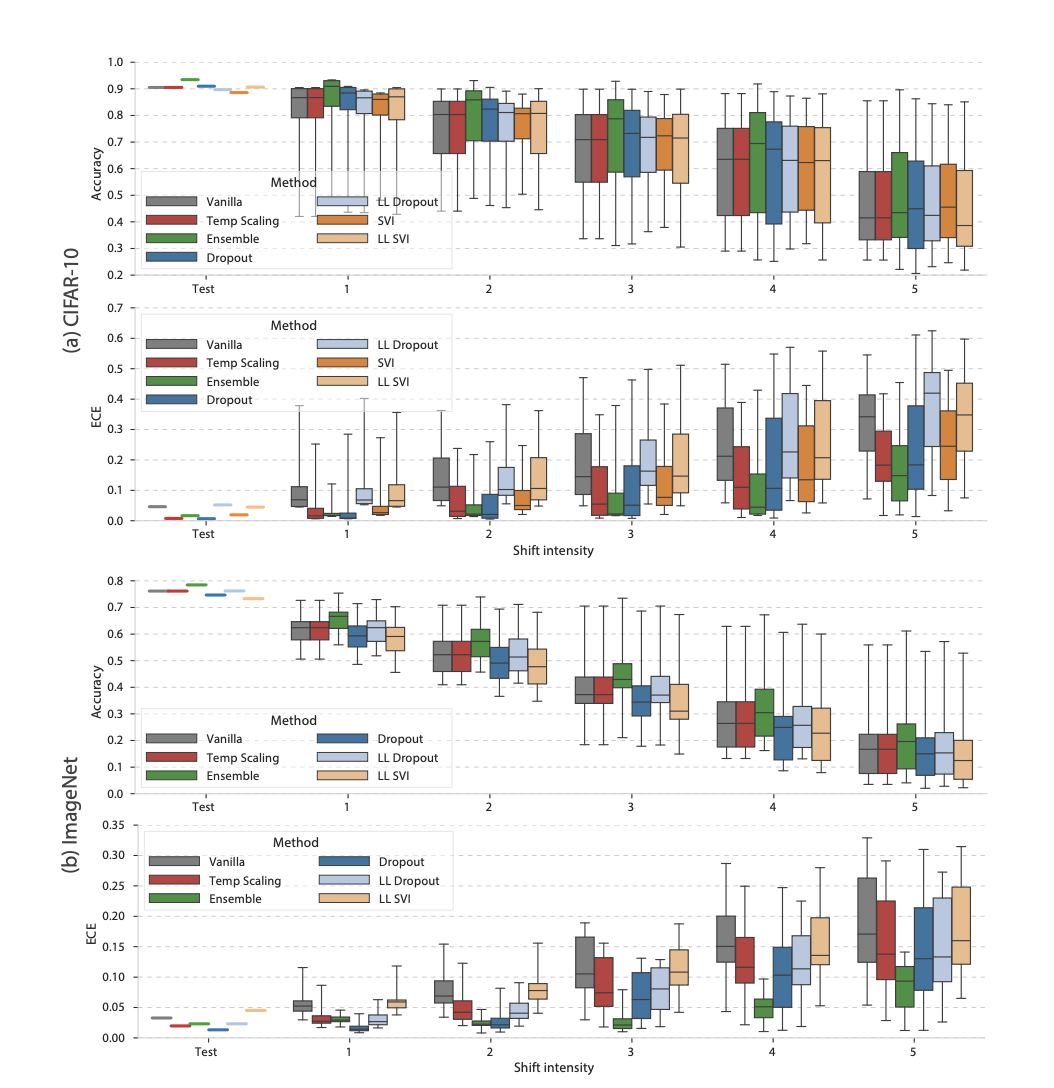
\includegraphics[scale=0.8]{figures/related_work/eval_uq_dataset_shift.png}
%    \caption{
%    % TODO: to be paraphrased
%    Calibration under distributional shift: a detailed comparison of accuracy and ECE under all types of corruptions on (a) CIFAR-10 and (b) ImageNet. For each method, the mean on the test set is shown, and summarise the results on each intensity of shift are with a box plot. Each box shows the quartiles summarising the results across all (16) shift types while the error bars indicate the min and max across different shift types\cite{evalUQDatasetShift}.
%    }
%    \label{fig:my_label}
%\end{figure}


%%%%%%%%%%%%%%%%%%%%%%%%%%%%%%%%%%%%%%%%%%%%%%%%%%%%%
%%%%%%%%%%%%%%%% scalable baselines %%%%%%%%%%%%%%%%%
%%%%%%%%%%%%%%%%%%%%%%%%%%%%%%%%%%%%%%%%%%%%%%%%%%%%%
\subsection{Scalable uncertainty quantification for deep learning} \label{model:scalable-DL}

% \subsection{Dropout as Bayesian Estimation}
% \subsection{Batch ensemble}
% \subsection{Rank 1 BNN}
In 2015, Gal Y. et al.\cite{dropoutDeepNets} demonstrated that training DNNs using Monte Carlo dropout could approximate Bayesian inference in deep Gaussian processes. Dropout at test time can therefore be used to generate an ensemble of predictions without the need to train independent models. On the other hand, SWAG\cite{SWAG} optimises the SGD and fits a Gaussian around the averaged weights, which is then assumed to be the posterior parameter distribution.
% Alternative approach
Alternative approaches to scale deep ensembles often propose to reduce the degree of independence between models and instead allow them to share some weights. Batch ensembles\cite{batchEnsemble} achieves competitive performance both in accuracy and uncertainty as deep ensembles at a factor 3 speedup and memory reduction (for an ensemble of size 4). Each weight matrix is defined as the Hadamard product of a shared weight among all ensemble members and a local rank-one factor matrix per member. Dusenberry et al.\cite{rank1BNN} extend the BatchEnsemble framework to be Bayesian over these factors, improving the quality of UQ. Finally, multi-inputs-multi-outputs\cite{MIMOEnsembles} architectures force the model to simultaneously give a prediction for a fixed set of $M$ inputs. During training, these $M$ inputs are sampled randomly from the training set and can be of different class labels. However, the same input is fed $M$ times to the model at test time to generate an ensemble of $M$ predictions, which can be used for UQ. This architecture tends to learn to access different sub-networks to generate a robust prediction.

\subsection{Uncertainty-driven adversarial perturbations} \label{model:udp}

Uncertainty-driven perturbations\cite{UDP} (UDP) are a type of adversarial perturbations constructed using gradient-ascent on the direction of maximal uncertainty for the model. They do not rely on input labels. They were introduced to reduce the simplicity bias of neural networks, i.e. the tendency to learn over-simple decision boundaries, which makes them vulnerable to small input perturbations. Classifiers trained to be robust against them tend to produce larger-margin decision boundaries, improving the model's generalisation.

%%%%%%%%%%%%%%%%%%%%%%%%%%%%%%%%%%%%%%%%%%%%%%%%%%%%%%%%%%%%%%%%%%
%%%%%%%%%%%%%%%%%%%%%%%%%%%%%%%%%%%%%%%%%%%%%%%%%%%%%%%%%%%%%%%%%%
%%%%%%%%%%%%%%%%%%%%%%%%%%%%%% NLP %%%%%%%%%%%%%%%%%%%%%%%%%%%%%%%
%%%%%%%%%%%%%%%%%%%%%%%%%%%%%%%%%%%%%%%%%%%%%%%%%%%%%%%%%%%%%%%%%%
%%%%%%%%%%%%%%%%%%%%%%%%%%%%%%%%%%%%%%%%%%%%%%%%%%%%%%%%%%%%%%%%%%

\section{Hallucinations, factuality and uncertainty in NLP}


% motivation on the rise of NLP application
% def of hallucination and factuality.
% describe metrics 
% overview of tasks specific progress: two roads 1) detect and correct and 2) build a more reliable system.

Despite the rise, popularity and performance of deep learning and transformers for NLP tasks, these models are often prone to hallucinations or, more generally, producing unintended and non-factual information. Hallucinations are crucial to detect or/and prevent because they can lead to inaccurate or misleading information, especially if the model has not been adequately trained or validated. Models generate outputs based on patterns seen during training, and hallucinations may occur due to old, noisy and inaccurate training data. Their occurrence is strongly impacted by the training dataset quality as hallucinations seen during training tend to be amplified by models during testing\cite{originHalluDataOrModel}. 
Xiao et al.\cite{hallucinationUQWang} establish parallels between uncertainty quantification and hallucinations. In particular, they showed that high uncertainty is correlated with high hallucination probability. In addition, they propose an uncertainty-aware beam search to reduce hallucinations during the decoding phase of conditional generation. 

\subsection{Hallucination detection}

%\cite{surveyHallucination}
\begin{figure}[!ht]
    \centering
    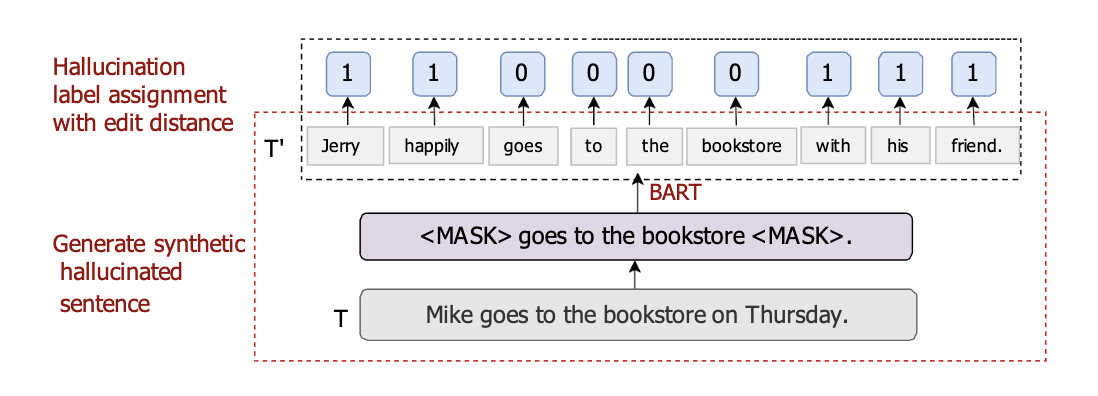
\includegraphics[scale=0.6]{figures/related_work/synthetic_hallu.png}.
    \caption{Generation of synthetic data with hallucination labels\cite{HallucationDetectionUsingSyntheticData}.}
    \label{fig:BART-synthetic-hallucination-creation}
\end{figure}

Zhou et al.\cite{HallucationDetectionUsingSyntheticData} suggest using a token-level hallucination detection task to evaluate the faithfulness of NLP models. To do so, they fine-tuned a language model using synthetic hallucination data and benchmarked their approach on machine translation (MT) and abstractive summarisation tasks. It achieved an average F1 score of 0.6 without requiring any supervised data. Consider an MT use case. Given an input sequence $G$ and its generated translation $T$, the detection task is formulated as a sequence labelling task: $((G, T), A_T)$ where $A_T$ is the sequence of binary hallucination labels for each token in $G$. The supervised labels $A_T$ are generated by replacing some tokens in $T$ with hallucinations. With this updated hallucinated sequence $\Tilde{T}$, the training set for hallucination detection becomes $((G, \Tilde{T}), A_T)$. In addition, they ensure that $\Tilde{T}$ remains coherent and similar to $T$ to reduce any bias at test time. The replacement tokens are produced by the BART model via masked tokens, as highlighted in figure \ref{fig:BART-synthetic-hallucination-creation}. The edit distance between $\Tilde{T}$ and $T$ is used to assign the $A_T$ labels.

\subsection{Factuality enhanced language models} \label{related-work:factuality-enhanced-LM}

%\cite{surveyFactualityGeneration}

Lee et al.\cite{factualityEnhancedLM} studied the factual accuracy of open-ended text generation use cases using large-language models. The faithfulness of models is evaluated through factual and non-factual prompts, as well as metrics such as the hallucination ratio. They rely on Wikipedia as a ground-truth knowledge base: first at document-level using the FEVER dataset and then at sentence-level via a best-similarity sentence procedure based on TF-IDF. Ultimately, their evaluation framework is composed of three phases.

First, check-worthy continuations are identified. They correspond to subsequences of the generated text for which a factuality test is necessary, i.e. expressions of knowledge. For example, personal opinions or chitchat style do not fall under that category and should, therefore, be skipped in the evaluation process. Then, for each check-worthy continuation, relevant ground-truth knowledge expressions are searched for in the knowledge base. Finally, factuality and quality measures are computed and reported.

Furthermore, they propose factual-nucleus sampling, an alternative decoding algorithm that incorporates a regularisation factor to classical nucleus sampling to account for factuality. This sampling algorithm was developed to limit the effects of “uniform randomness” that suffer popular sampling algorithms, which tend to undermine factuality.

\subsection{Uncertainty in sequence-to-sequence models}

Uncertainty in text generation and language models comes under different forms. One reflects that the same input sequence can usually be paired with multiple correct output sequences, as is often the case in machine translation tasks. Additionally, decoding strategies impact uncertainty as different search algorithms will result in different prediction probabilities and, therefore, uncertainty. 

Stahlberg et al.\cite{uncertaintyNLPandDecoding} reflect on the implications of intrinsic uncertainty on the inductive biases in beam search, as well as the complexity of the exact search. Two tasks with different uncertainty levels are studied:  machine  translation  (MT) for high uncertainty and  grammatical  error  correction  (GEC) for low uncertainty. 
In this work, uncertainty is measured as the edit distance between multiple reference tasks. It was demonstrated that many common issues with decoding algorithms only arise for MT or, more generally, uncertain tasks. For instance, beam search errors and performance drops due to large beam sizes are explored. To address some of these issues, they proposed a new exact $n$-best search algorithm based on a set of $n$ best hypotheses. If this set covers a high enough fraction of the total probability mass, it can accurately approximate the model distribution.


%%%%%%%%%%%%%%%%
\chapter{Design} \label{chatper:design}
%%%%%%%%%%%%%%%%

%Introduce and discuss the design decisions that you made during this project.
%Highlight why individual choices are important and/or necessary. Discuss
%how the design fits together.

%This section is usually 5-10 pages.

%%%%%%%%%%%%%%%%%%%%%%%%%%%%%%%%%%%%%%%%%%%%%%%%%%%%%%%%%%%%

%Multiple individual contributions:
%* Ensemble aggregation methods to evaluate model uncertainty.
%* Experiments on the effect of class imbalance on UQ performance.
%* OOD evaluation of models using adversarial perturbations

%2nd part:
%  - Focus on NLP and hallucinations of LM.=

This chapter first covers the models implemented in the standardised UQ package to estimate data and model uncertainty. Then, models specific to NLP, sequence-to-sequence and graph-to-text models are described.  


\section{General uncertainty quantification models} \label{design:uq-models}

Due to the \textit{scikit-learn} constraints of the package to be developed, the following base models are considered: Logistic Regression, Linear Regression, Gaussian Processes, Gradient-Boosted Trees, Random Forest and  Gaussian Mixture Models. In this work, a base model corresponds to a model for which uncertainty quantification shall be performed. 

%\subsection{Data UQ}

For classification, data uncertainty is measured by the entropy of the prediction distribution $\Entropy_i = - \sum_k \log p_{i,k}$ for data point $x_i$. For regression, one of probabilistic regression (cf. \ref{model:probabilistic-learning}), ensemble-based models (cf. \ref{model:ensembles}) or quantile regression (cf. \ref{model:quantile-regression}) is considered depending on the base model used. 

To estimate model uncertainty, more than one standalone model is required. To solve this issue, ensembles are used in this work, as shown in section \ref{section:background:ensembles}. Different types of ensembles are considered: seed ensemble, hyper-parameter ensemble, bagging ensemble and adversarial ensemble. The latter is the only model not introduced in section \ref{model:ensembles}.

\section{Adversarial ensembles} \label{section:design:adversarial}
Consider a set of adversarial attacks $\mathcal{A} = \{A_1, \ldots, A_L\}$ and the adversarial training procedure in algorithm \ref{alg:adversarial-training}. Ensemble adversarial training trains $M$ of these models independently and aggregates their predictions. Attacks are defined as functions that produce perturbations $\delta = A(D)$ when given as input a dataset $D = (X,Y) = \{(x_i, y_i)\}_i$. Some attacks do not require the $\{y_i\}_i$ labels.

\begin{algorithm}
\caption{Adversarial training.}\label{alg:adversarial-training}
\begin{algorithmic}

\Require $f_{\theta}$ and $D_{train} = (X,Y)$ \Comment{model function and training data set}
\Require $\mathcal{A}$ \Comment{set of adversarial attacks}
\Require $\eta$ \Comment{number of adversarial training epochs}
%\State $y \gets []$
\For{$i \gets 1$, $\eta$}
    \State $A = Sample(\mathcal{A})$
    \State $\delta = A(D_{train})$
    \State $\Tilde{X} = X + \delta$  
    \State $train(f_{\theta}, \Tilde{X})$ \Comment{train the model for a few epochs}
\EndFor
\end{algorithmic}
\end{algorithm}

However, an attack on such ensembles can not be carried out using gradient methods on the ensemble as a whole. Instead, attacks have to be placed on individual members of the ensemble. Let $\mathcal{A} = \{A_1, \ldots, A_M\}$ be a set of $M$ attacks, each placed on a single model, i.e. $A_m$ generates perturbations fooling model $f_m$. An ensemble attack can be defined as:
$$
\delta_{ensemble} = A_{ensemble}(D) = g(A_1(D), \ldots A_M(D)) = g(\delta_1, \ldots, \delta_M)
$$

$g$ is an aggregation function which can either be the mean, the median, the maximum, or a uniform random sample, etc. For instance:
$
g_{mean}(\delta_1, \ldots, \delta_M)_d = \frac{1}{M} \sum_i \delta_{i,d}
$
or
$
g_{random}(\delta_1, \ldots, \delta_M) = \delta_{W}\; \text{such that} \;  W \sim Uniform(1,M)
$.


\section{UQ models for graph-to-text} \label{design:UQ-models-G2T}

Sequence-to-sequence transformers such as T5 are composed of an encoder and a decoder part. For our use case, the quantity of interest is the uncertainty of the natural language generation task. Assuming that the encoder builds an accurate embedding for the input graph, the focus can be placed on the decoding phase with respect to UQ. As declared in section \ref{intro:problem-section}, the aim of UQ models is to produce uncertainty scores at token-level for the prediction texts. Of course, these sources can easily be aggregated at higher granularity, e.g. words or sentences. 

\subsection{Prediction entropy sequence} \label{models:entropy-sequence}

In UQ for classification, the primary quantity of interest is the entropy of the prediction distribution, i.e. SoftMax outputs for the target variable. In text generation, prediction is not about a single variable but rather a causal sequence of tokens $\{t_j\}_{j=1}^L$ defined in the simple case of greedy decoding, by 
$
    t_j = \argmax_k \; p_{j,k} = \argmax_k \; P[t_k \mid t_{j-1}, t_{j-2}, \ldots, t_{0}]
$.

The equivalent notion of predicted entropy for text generation is the predicted entropy sequence $\{\Entropy_j\}_{j=1}^L$, defined as $\Entropy_j = \Entropy(p_j) = - \sum_k p_{j,k} \log p_{j,k} $.

\subsection{Ensembles}

As earlier sections demonstrate, ensembles are essential to improve uncertainty quantification models. The following types are considered:

\begin{enumerate}
    \item Deep ensemble: multiple independent copies of a base model are trained on the same dataset, using different seeds. In previous sections, this model was also called seed ensemble. 
    \item Dropout ensemble: T5 was pre-trained using dropout. If fine-tuning is performed using the same dropout strategy, dropout can be used at test time to generate multiple predictions and approximate model uncertainty (cf. section \ref{model:scalable-DL}).
    \item \label{model:graph-encoding-ensemble} Graph encoding ensemble: the first step of the current graph-to-text pipeline is to linearise the graph into an ordered sequence of edges. This sequence is then passed to the T5 sequence-to-sequence model to generate the final textual representation of the graph. However, there are $|E|!$ possible orderings, which all represent the same graph. Therefore, ensembling a few predictions based on different linearisation can provide a further method to quantify the uncertainty related to the input graph.
\end{enumerate}

However, it remains to discuss how these different predictions should be aggregated to produce an uncertainty score. The aggregation can be performed at two different levels. First, consider the aggregation at text-level. Each model $m$ predicts a natural textual output $T^m$, and each of them is composed of an independent sequence of tokens $\{t_j^m\}_{j=1}^{n_m}$. One possible output aggregation strategy is explained below:
    \begin{enumerate}
        \item Choose a reference output $T^*$ among $\{T^m\}_{m=1}^M$. For instance, it could be the text with the highest probability (or lowest perplexity).
        \item For each output $T^m$ where $m \not= *$, use a string sub-sequence matching algorithm between $T^*$ and $T^m$ to highlight which characters/tokens of $T^m$ are in agreement with $T^*$. Let $a_j^m = 1$ if that is the case and $a_i^m = 0$ otherwise.
        \item For each character/token $t_j^m$, the uncertainty score is defined as $\frac{1}{M} \sum a_i^m$.
    \end{enumerate}
This approach is only valid under the assumption that the outputs $\{T^m\}_{m=1}^M$ are very similar, which is the case for some of the datasets considered in this work. Several tests were conducted on this aggregation type, and we realised that many errors were introduced during the matching phase. In the end, the alternative token-level aggregation was selected as the method of choice. In this approach, consider the prediction token distributions produced by each ensemble member.

$$
p_{j,k}^m = P[t_k^m \mid t_{j-1}, t_{j-2}, \ldots, t_{0}] \;\;\; \forall k=0,1,\ldots, |V|
$$

They can be averaged to create the average ensemble distribution $\bar{p}_{j,k} = \frac{1}{M} \sum_m p_{j,k}^m$
and the associated entropy sequence $\{H(\bar{p}_{j}) \}_{j=1}^L$. To construct the individual member distributions $p_{j,k}^m$, a reference model, e.g. $m=1$ is first selected to generate a reference predicted token sequence $T^1 = \{t_{j}^1\}_{j=1}^L$ with associated token distribution $\{p_{j,k}^1\}_{j,k}$. The other members $m=2, \ldots, M$ are then forced to regenerate $T^1$ using the modified decoding procedure available in algorithm \ref{alg:targeted-decoding}, named targeted decoding. To implement this method, it is required to modify the transformers library's decoding algorithms (greedy search, beam search, etc.). More generally, targeted decoding can be valuable in studying the predicted probability distribution of user-defined token sequences instead of relying on the model to generate them. 

\begin{algorithm}
\caption{Targeted decoding.}\label{alg:targeted-decoding}
\begin{algorithmic}

\Require $f$, $X$,  $t_j \;\forall \; j=1, \ldots, j=L$   \Comment{model function, input sequence and target tokens.}
\State $y$, $p$, $h \gets EmptyList$
\State $y.append(StartSequenceToken)$
\State $j \gets 1$
\While{$j \leq L$}
    \State $y.append(t_j)$  \Comment{Generate the same token as the target tokens}
    \State $s \gets f_j(X, y)$  \Comment{Causal token prediction using input and partial output}
    \State $p_j \gets Softmax(s)$
    \State $p.append(p_j)$
    \State $h.append(Entropy(p_j))$ \Comment{Compute entropy}
    \State $j \gets j + 1$
\EndWhile
\State \Return $y$, $p$, $h$
\end{algorithmic}
\end{algorithm}


\subsection{Synthetic data creation for token-level hallucination detection} \label{design:synthetic-hallucination-data}


\begin{figure}[t]
    \centering
    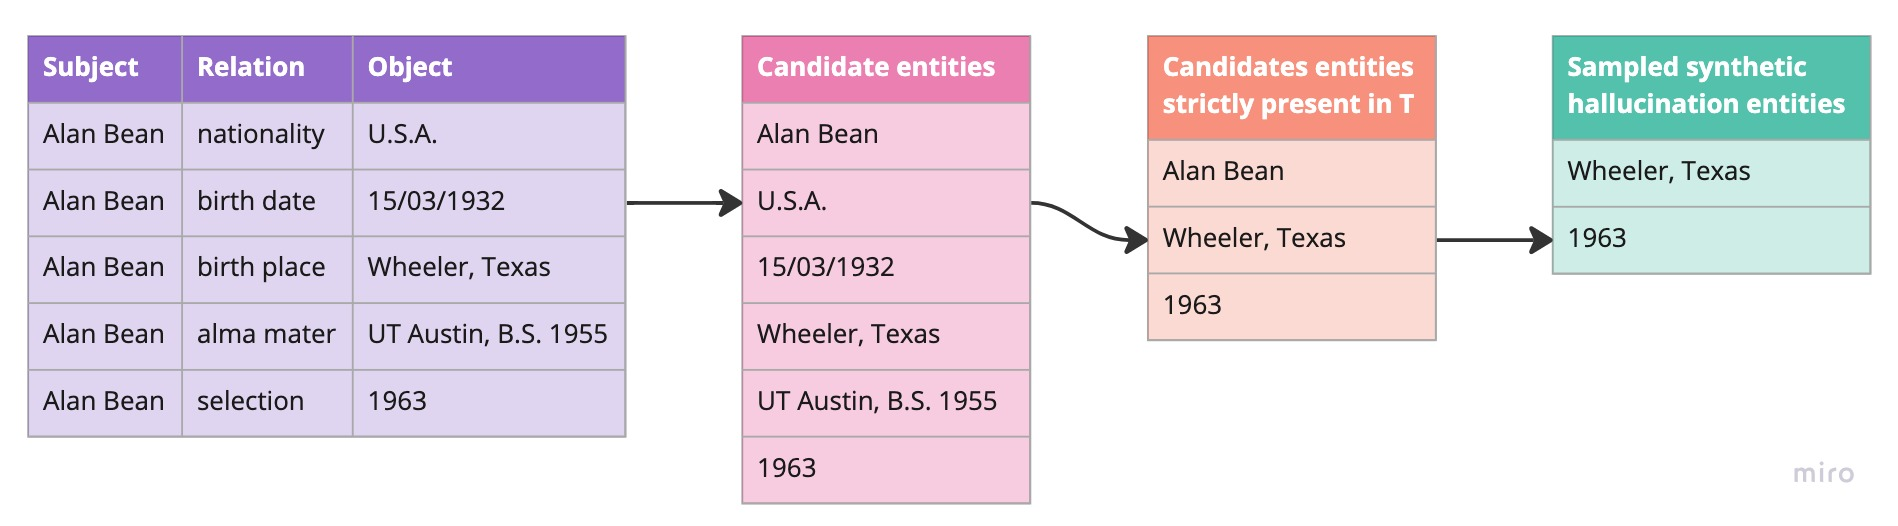
\includegraphics[scale=0.23]{figures/design/synthetic/hallu_ents_selection.jpg}
    \caption{Phase (a). Synthetic hallucination entities generation, i.e. $\tilde{C}_G$.}
    \label{fig:synthetic-ents-selection}
\end{figure}

In this section, the focus is placed on graph-to-text datasets. Modified versions of the datasets introduced in section \ref{section:datasets} are built to study hallucinations due to missing edge information. Unlike other NLP tasks, hallucinations in data-to-text models can often be checked using the input data, which acts as an internal knowledge base. Hallucinations are defined at token-level: for each token $t_j$ in the prediction text $T$, a binary label $a_j$ is assigned. It indicates whether it corresponds or not to a hallucination. 

Zhou et al.\cite{HallucationDetectionUsingSyntheticData} proposed a method to generate a similar synthetic labelled dataset for token-level hallucination in a machine translation context. However, they introduced hallucinations by updating some tokens in the prediction texts. A different approach is undertaken in this work that does not require any modification to the reference or prediction texts. The hallucinations are introduced by dropping meaningful pieces of information from the input sequence so that factual errors naturally occur in the output sequence. 

% The intuition is that some information necessary to generate a piece of text has been removed from the input data. Therefore, concerning the new dataset, this information corresponds to a hallucination. 

%The synthetic data creation is defined as follows
Consider a graph and text pair $(G, T)$. The first phase of the synthetic data generation process is to create $C_G$, a set of candidate hallucination entities from $G$. It consists of all subjects and objects contained in the edges of $G$, i.e. $C_{G} = \bigcup_{e \in G} \{subject(e), object(e)\}$. Then entities that are not strictly present in $T$ are filtered out. For example, if a date $15/03/1932$ is a candidate entity but is only present in $T$ in a written format such as March 15, 1932, it will not be considered anymore. This ensures a low matching error between the entities in $C_G$ and the entities in $T$. From $C_G$,  $K < |C_G|$ entities are sampled and stored in $\Tilde{C}_G$. The latter is the final hallucination entity set. Sub-sampling avoids creating an overly large number of hallucinations which would lead to inconsistencies in the dataset. Figure \ref{fig:synthetic-ents-selection} illustrates this process via the graph-to-text example of section \ref{background:G2T}.

\begin{figure}
    \centering
    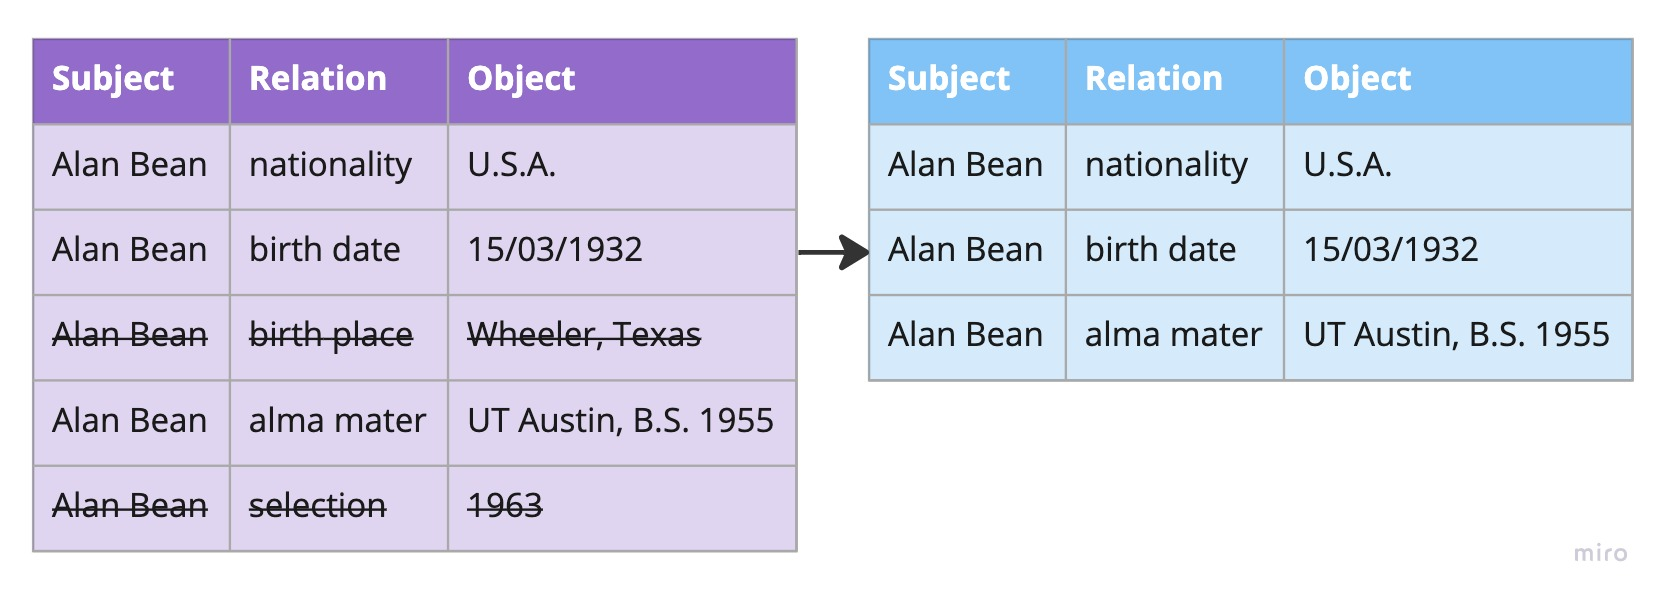
\includegraphics[scale=0.2]{figures/design/synthetic/hallu_graph.jpg}
    \caption{Phase (b). Synthetic hallucination graph generation, i.e. $\Tilde{G}$.}
    \label{fig:synthetic-hallu-graph}
\end{figure}

\begin{figure}
    \centering
    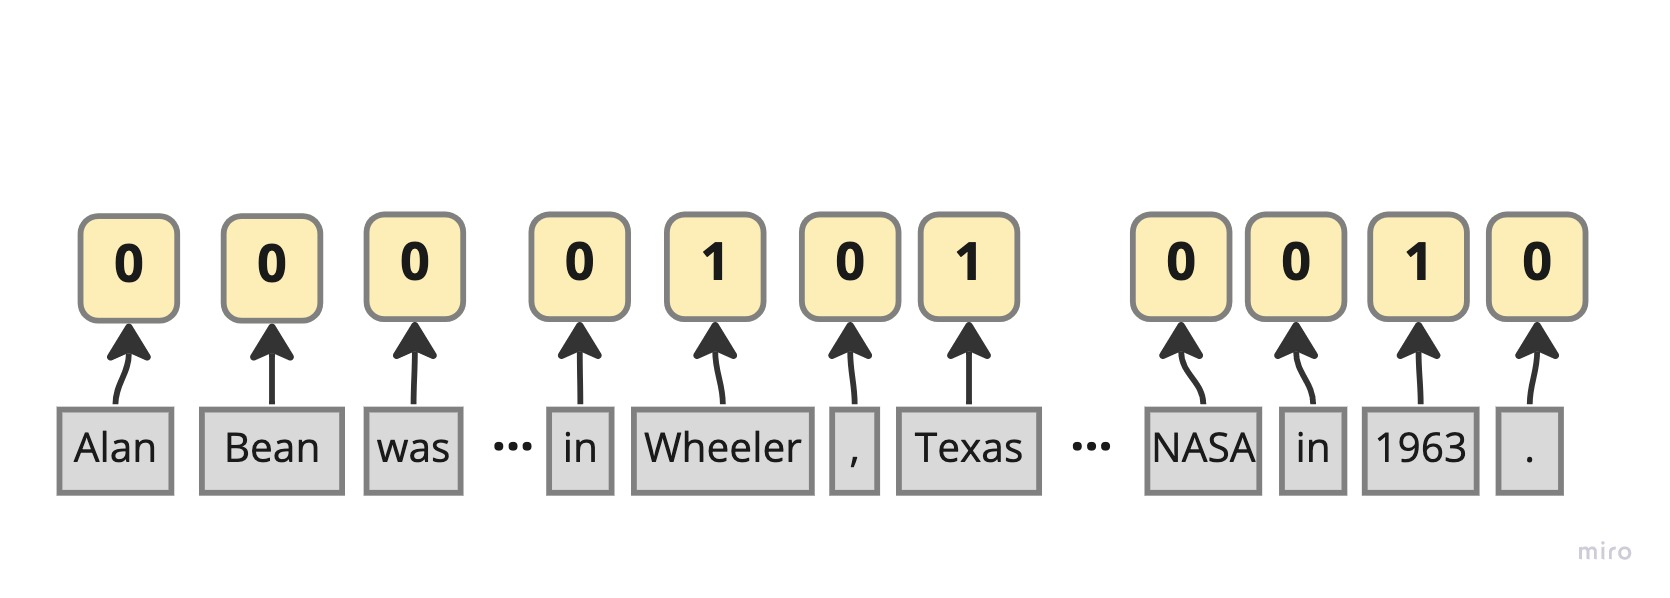
\includegraphics[scale=0.18]{figures/design/synthetic/hallu_labels.jpg}
    \caption{Phase (c). Synthetical hallucination labels generation, i.e. $\{a_j\}_j$.}
    \label{fig:synthetic-hallu-labels}
\end{figure}
\newpage
Based on $\Tilde{C}_G$, let $\Tilde{G} = \{e \in G \,:\, subject(e) \not\in \Tilde{C}_G \;\land\; object(e) \not\in \Tilde{C}_G\}$ be the graph containing only edges without hallucination. This constitutes the second step of the generation pipeline, and it can be visualised in figure \ref{fig:synthetic-hallu-graph}. Finally, the synthetic labels are defined as $a_{j} = I\{\exists_k \;:\; t_j \in c_k, \; c_k \in \Tilde{C_G}\}$ and are highlighted in figure \ref{fig:synthetic-hallu-labels}. This procedure can be generalised to all pairs $(G_i, T_i)$ so that $a_{i,j}$ corresponds to the hallucination label for the $j^{th}$ token of the $i^{th}$ text. It is also convenient to define the graph-to-text hallucination dataset $\Tilde{D} = \{(\Tilde{G_i}, T_i, a_{i, \cdot})\}_{i=1}^N$.

As a post-processing step, all hallucination labels $a_{i,j} = 1 $ corresponding to stop words are reset to non-hallucinations, i.e. $a_{i,j} = 0$. This ensures that hallucinations are only composed of pure expression of knowledge in the reference texts. For each $G_i$, $K$ is set so that roughly $1/3$ of the edges of the graph are dropped using this procedure.  

\subsection{Hallucination detection models} \label{design:hallucination-detection-models}
%Carefully chosen pieces of information are removed from the input graph to force models to generate hallucinations. 

The synthetic dataset described in section \ref{design:synthetic-hallucination-data} provides an extra set of labels for hallucination detection for graph-to-text. The latter can be used to analyse models trained to perform hallucination detection at token-level, i.e. for each token $t_j$ of each text $T_i$, a binary prediction $\hat a_{ij}$ has to be produced.

To this end, different hallucination detection approaches are compared. A detection baseline is constructed using the evaluation pipeline of Lee et al.\cite{factualityEnhancedLM} described in section \ref{related-work:factuality-enhanced-LM}. They use named-entity recognition to detect relevant factual information in the input graph and generated text. Furthermore, in a data-to-text use case, one can argue that the reference text should only contain factual information or expression of knowledge, e.g. no personal opinion or chitchat sentences. Hence, the check-worthy continuations identification step is less relevant here. In addition, the knowledge base can be restricted to the input data in graph-to-text applications. Particular emphasis is also placed on numeral hallucinations so that all text-like tokens (according to the spaCy library) in the prediction are considered valid expressions of knowledge and should therefore be checked for hallucination. Some efforts were made to reduce the number of false positives in their hallucination-checking phase by introducing a set of equivalents entities to be checked. For instance, shorter forms of country names and locations were not handled properly, e.g. USA, US, U.S.A., United States, similarly for quantities (e.g. 1 kg, 1000 g, 1.0 kg), dates (e.g. 17 June 2010, 17/06/2010, 17-06-2010), inhabitants and countries (e.g. Swiss, Switzerland), etc.   

The second hallucination detection model is directly based on the synthetic hallucination dataset. A logistic regression model is trained to detect hallucinations at token-level using entropy as the sole feature. The objective of this experiment is not to reach top-level performance but rather to quantify the predictive power of entropy for the hallucination detection task. Several variations of entropy as a feature are considered:
\begin{enumerate}
    \item Total entropy. It can be further decomposed into data and model uncertainty features to analyse which component has the strongest impact on hallucination occurrence. 
    \item Entropy of the $L$ previous tokens to introduce a dependence on past sequence elements. Since the hallucinations are synthesised at word-level and then expanded into tokens, one hallucination token is likely followed by a few additional ones. 
\end{enumerate}

For readability reasons, token-level predictions can also be aggregated at word-level using the following policy: a word is considered to be a hallucination if any of the tokens composing it is a hallucination. Given a predicted hallucination probability sequence $P = \{p_j\}_j$ corresponding to the tokens $T = \{t_j\}_j$, the word expansion of $P$, $\Tilde{P}$ is defined by 

$$
\Tilde{p_j} = \argmax_{t_l \in word(t_j)} p_l\;\;\; \forall\; j = 1, \ldots, L
$$
$$
words(t_j) = \{t_l \;:\; t_l \;\text{and}\; t_j \;\text{belong to the same word}\; \forall\;l=1,\ldots,L\}
$$

Since the hallucination labels $\hat a_{ij}$ are constructed at word-level, word expansion as a post-processing step for a token-level detection model is expected to increase its performance.


%%%%%%%%%%%%%%%%%%%%%%%%
\chapter{Implementation}  \label{chatper:implementation}
%%%%%%%%%%%%%%%%%%%%%%%%

%The implementation covers some of the implementation details of your project.
%This is not intended to be a low-level description of every line of code that
%you wrote but covers the implementation aspects of the projects.

%This section is usually 3-5 pages.

\section{Framework overview}

\subsection{API requirements} \label{implementation:api-requirements}

The main requirement for developing the uncertainty quantification package is the \textit{scikit-learn} compatibility which imposes constraints on how the models are created, trained and evaluated. In particular, all models should implement the \textit{fit} and \textit{predict} functions as well as \textit{predict\_proba} for classification models. To ensure full compatibility with the \textit{scikit-learn} library (e.g. grid search, etc.), several other development guidelines should be followed, such as the instantiation rule: "every keyword argument accepted by \textit{\_\_init\_\_} should correspond to an attribute on the instance.". Such guidelines are made available to \textit{scikit-learn} contributors at this \href{https://scikit-learn.org/dev/developers/develop.html}{link} and were taken into consideration during the development phase. 

% explain target API return_std
In the context of uncertainty quantification, a few regression models capable of deriving uncertainty scores are already available in the \textit{scikit-learn} API: \href{https://scikit-learn.org/stable/modules/generated/sklearn.gaussian_process.GaussianProcessRegressor.html#sklearn.gaussian_process.GaussianProcessRegressor}{Gaussian Process regressor}, \href{https://scikit-learn.org/stable/modules/generated/sklearn.linear_model.BayesianRidge.html#sklearn.linear_model.BayesianRidge}{Bayesian Ridge regressor} and \href{https://scikit-learn.org/stable/modules/generated/sklearn.linear_model.ARDRegression.html#sklearn.linear_model.ARDRegression}{Automatic Relevance Determination regressor (ARD)}. The UQ API chosen by these models is articulated around the \textit{predict} function:


\begin{lstlisting}[language=Python, caption=UQ sklearn API.]
    mean_pred, std_pred = model.predict(X, return_std=True)
\end{lstlisting}

A default parameter \textit{return\_std} is added to the prediction function. If set to true, the function returns a tuple of arrays: the mean predictions and their standard deviations. This API is extended to all predictors, i.e. classifiers and regressors in the package. To make a clear distinction between data and model uncertainty, the following syntax is adopted: 

\begin{lstlisting}[language=Python, caption=Extraction of uncertainty scores from predictions.]
    # Task 1: data UQ regression
    uq_preds = data_uq_regressor.predict(X, return_std=True)
    preds, std = uq_preds[:, 0], uq_preds[:, 1]
    # Task 2: data UQ classification
    uq_preds = data_uq_clf.predict(X, return_std=True)
    preds, entropy = uq_preds[:, 0], uq_preds[:, 1]
    # Task 3: model UQ estimator (regression or classification)
    preds, std = model_uq.predict(X, return_std=True)
\end{lstlisting}

The output of a data UQ model is a 2D array containing the mean predictions in the first column and the uncertainty scores in the second. Model UQ predictions are tuples as defined in scikit-learn. Furthermore, several utility functions are made available to the users to produce confidence internals, conformal predictions, calibration, uncertainty plots, etc.

\subsection{Architecture}

The package is organised as a set of predictor wrappers which all take a base predictor as the main argument and return an updated predictor following the API requirements defined in section \ref{implementation:api-requirements}. %An overview of the data uncertainty regressor and classifier wrappers is shown in figure \ref{fig:diagram-data-uq-wrappers}. 
Calibration, model UQ and data UQ wrappers are meant to be chained one on top of the others as highlighted in figure \ref{fig:diagram-uq-wrappers} and code below. The \textit{fit} method only needs to be called on the top-level wrapper to train all subsequent ones. 
A hierarchy of the different classes implemented in the package is shared in figure \ref{fig:class-hierarchy}. 

\begin{lstlisting}[language=Python, caption=Extraction of uncertainty scores from predictions.]
    uq_model = CalibratedRegressorCV(
        ModelUQWrapper(DataUQWrapper(base_estimator))
    ).fit(X_train, y_train)
    preds, std = uq_model.predict(X_test, return_std=True)
\end{lstlisting}


%Sklearn abstract class & Base estimator                         & BaseEnsemble
%UQlearn abstract class & PredictWrapper                         & BaseEnsembleUQ
%UQlearn base class     & RegressorWrapper & ClassifierWrapper   & EnsembleUQRgressorWrapper & EnsembleUQClassifierWrapper
%UQlearn specifics      & QuantileRegressor & BayesianRgressorWrapper  & CatBoostRegressorWrapper & EnsembleRegressorWrapper & AdversarialClassifier & % BaggingUQRegressor & BaggingUQClassifier & AdversarialEnsembleUQClassifier 





\begin{figure}[h!]
    \centering
    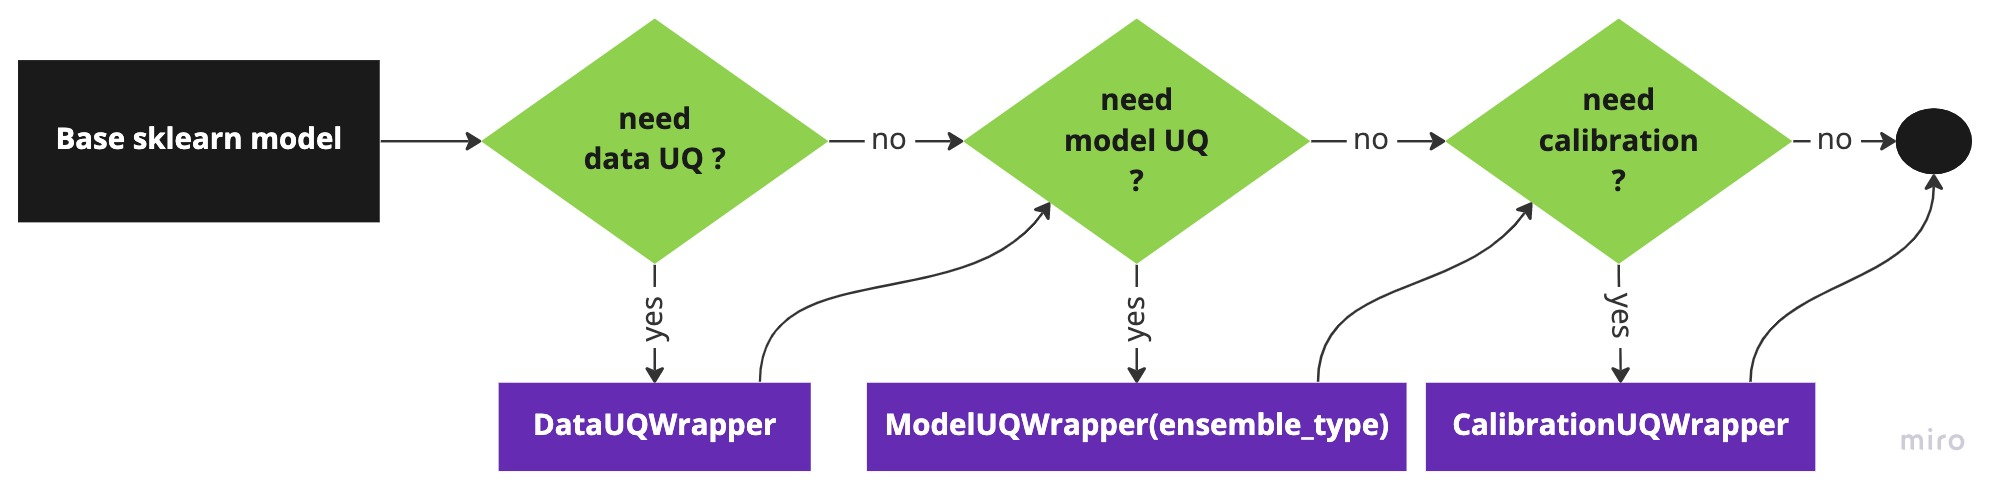
\includegraphics[width=.8\linewidth]{figures/implementation/diagram-sequence-wrappers.jpg}
    \caption{Schematic view of UQ wrappers and how they are built one on the other.}
    \label{fig:diagram-uq-wrappers}
\end{figure}

%\begin{figure}[htbp]
%    \centering
%    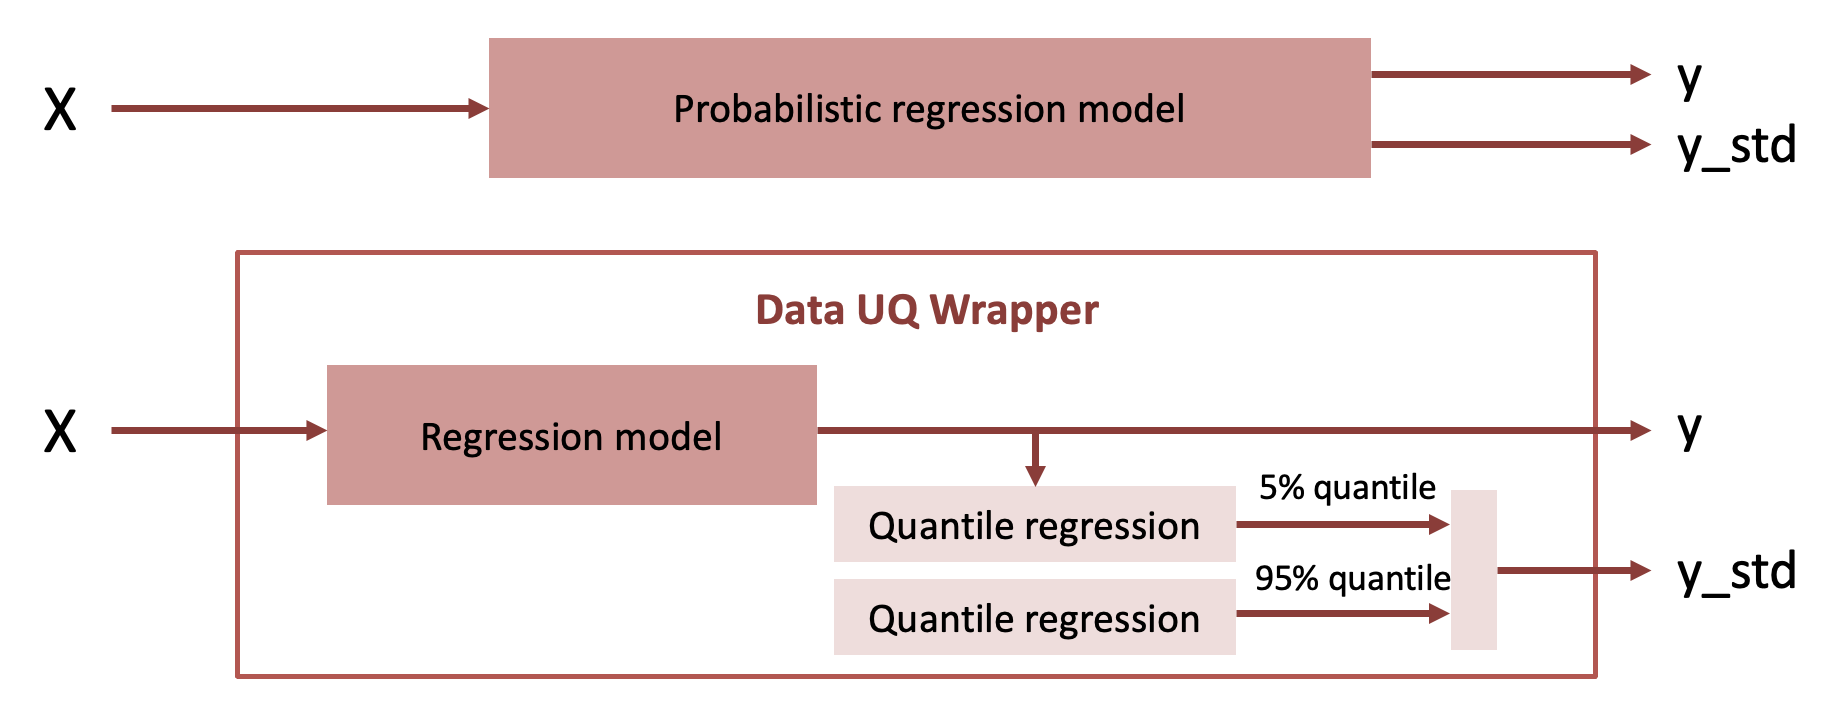
\includegraphics[width=.6\linewidth]{figures/implementation/diagram-uq-regressor.png}
%    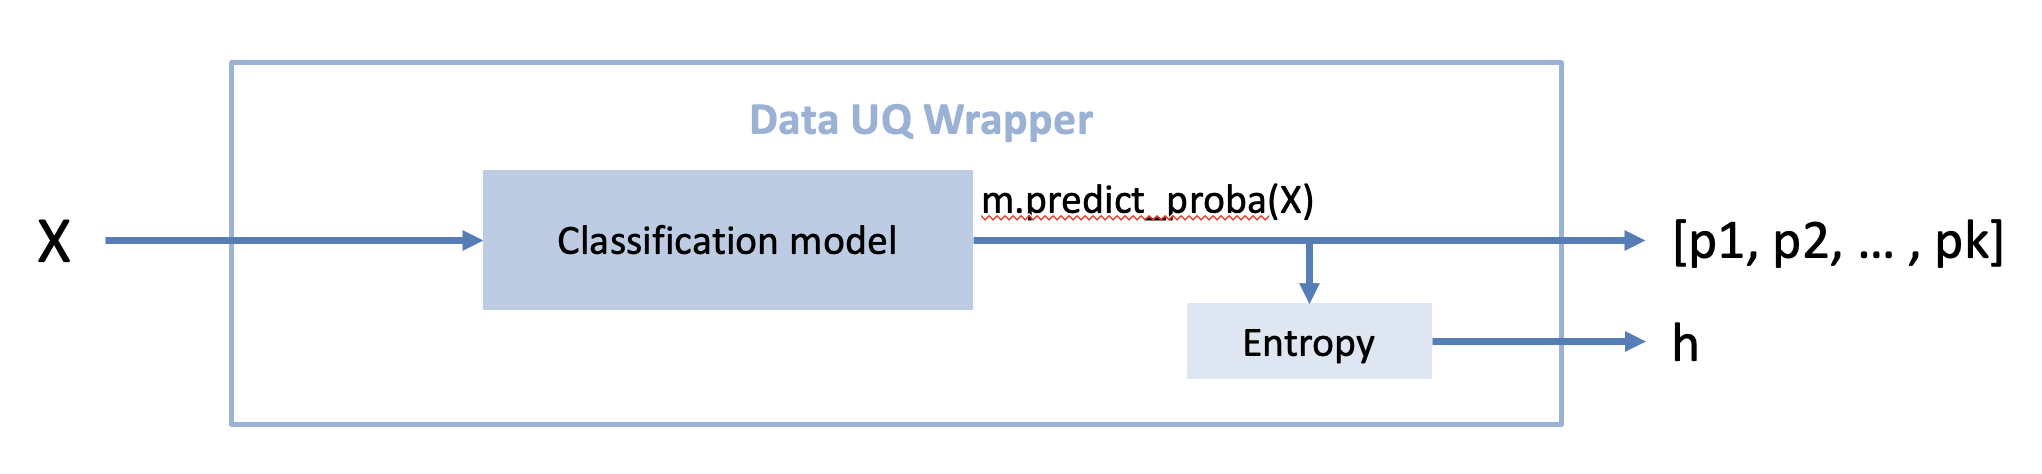
\includegraphics[width=.6\linewidth]{figures/implementation/diagram-uq-classifier.png}
%    \caption{Schematic view of data UQ wrappers (classification and regression).}
%    \label{fig:diagram-data-uq-wrappers}
%\end{figure}

\begin{figure}[htbp]
     \centering
     \begin{subfigure}[b]{0.32\textwidth}
         \centering
         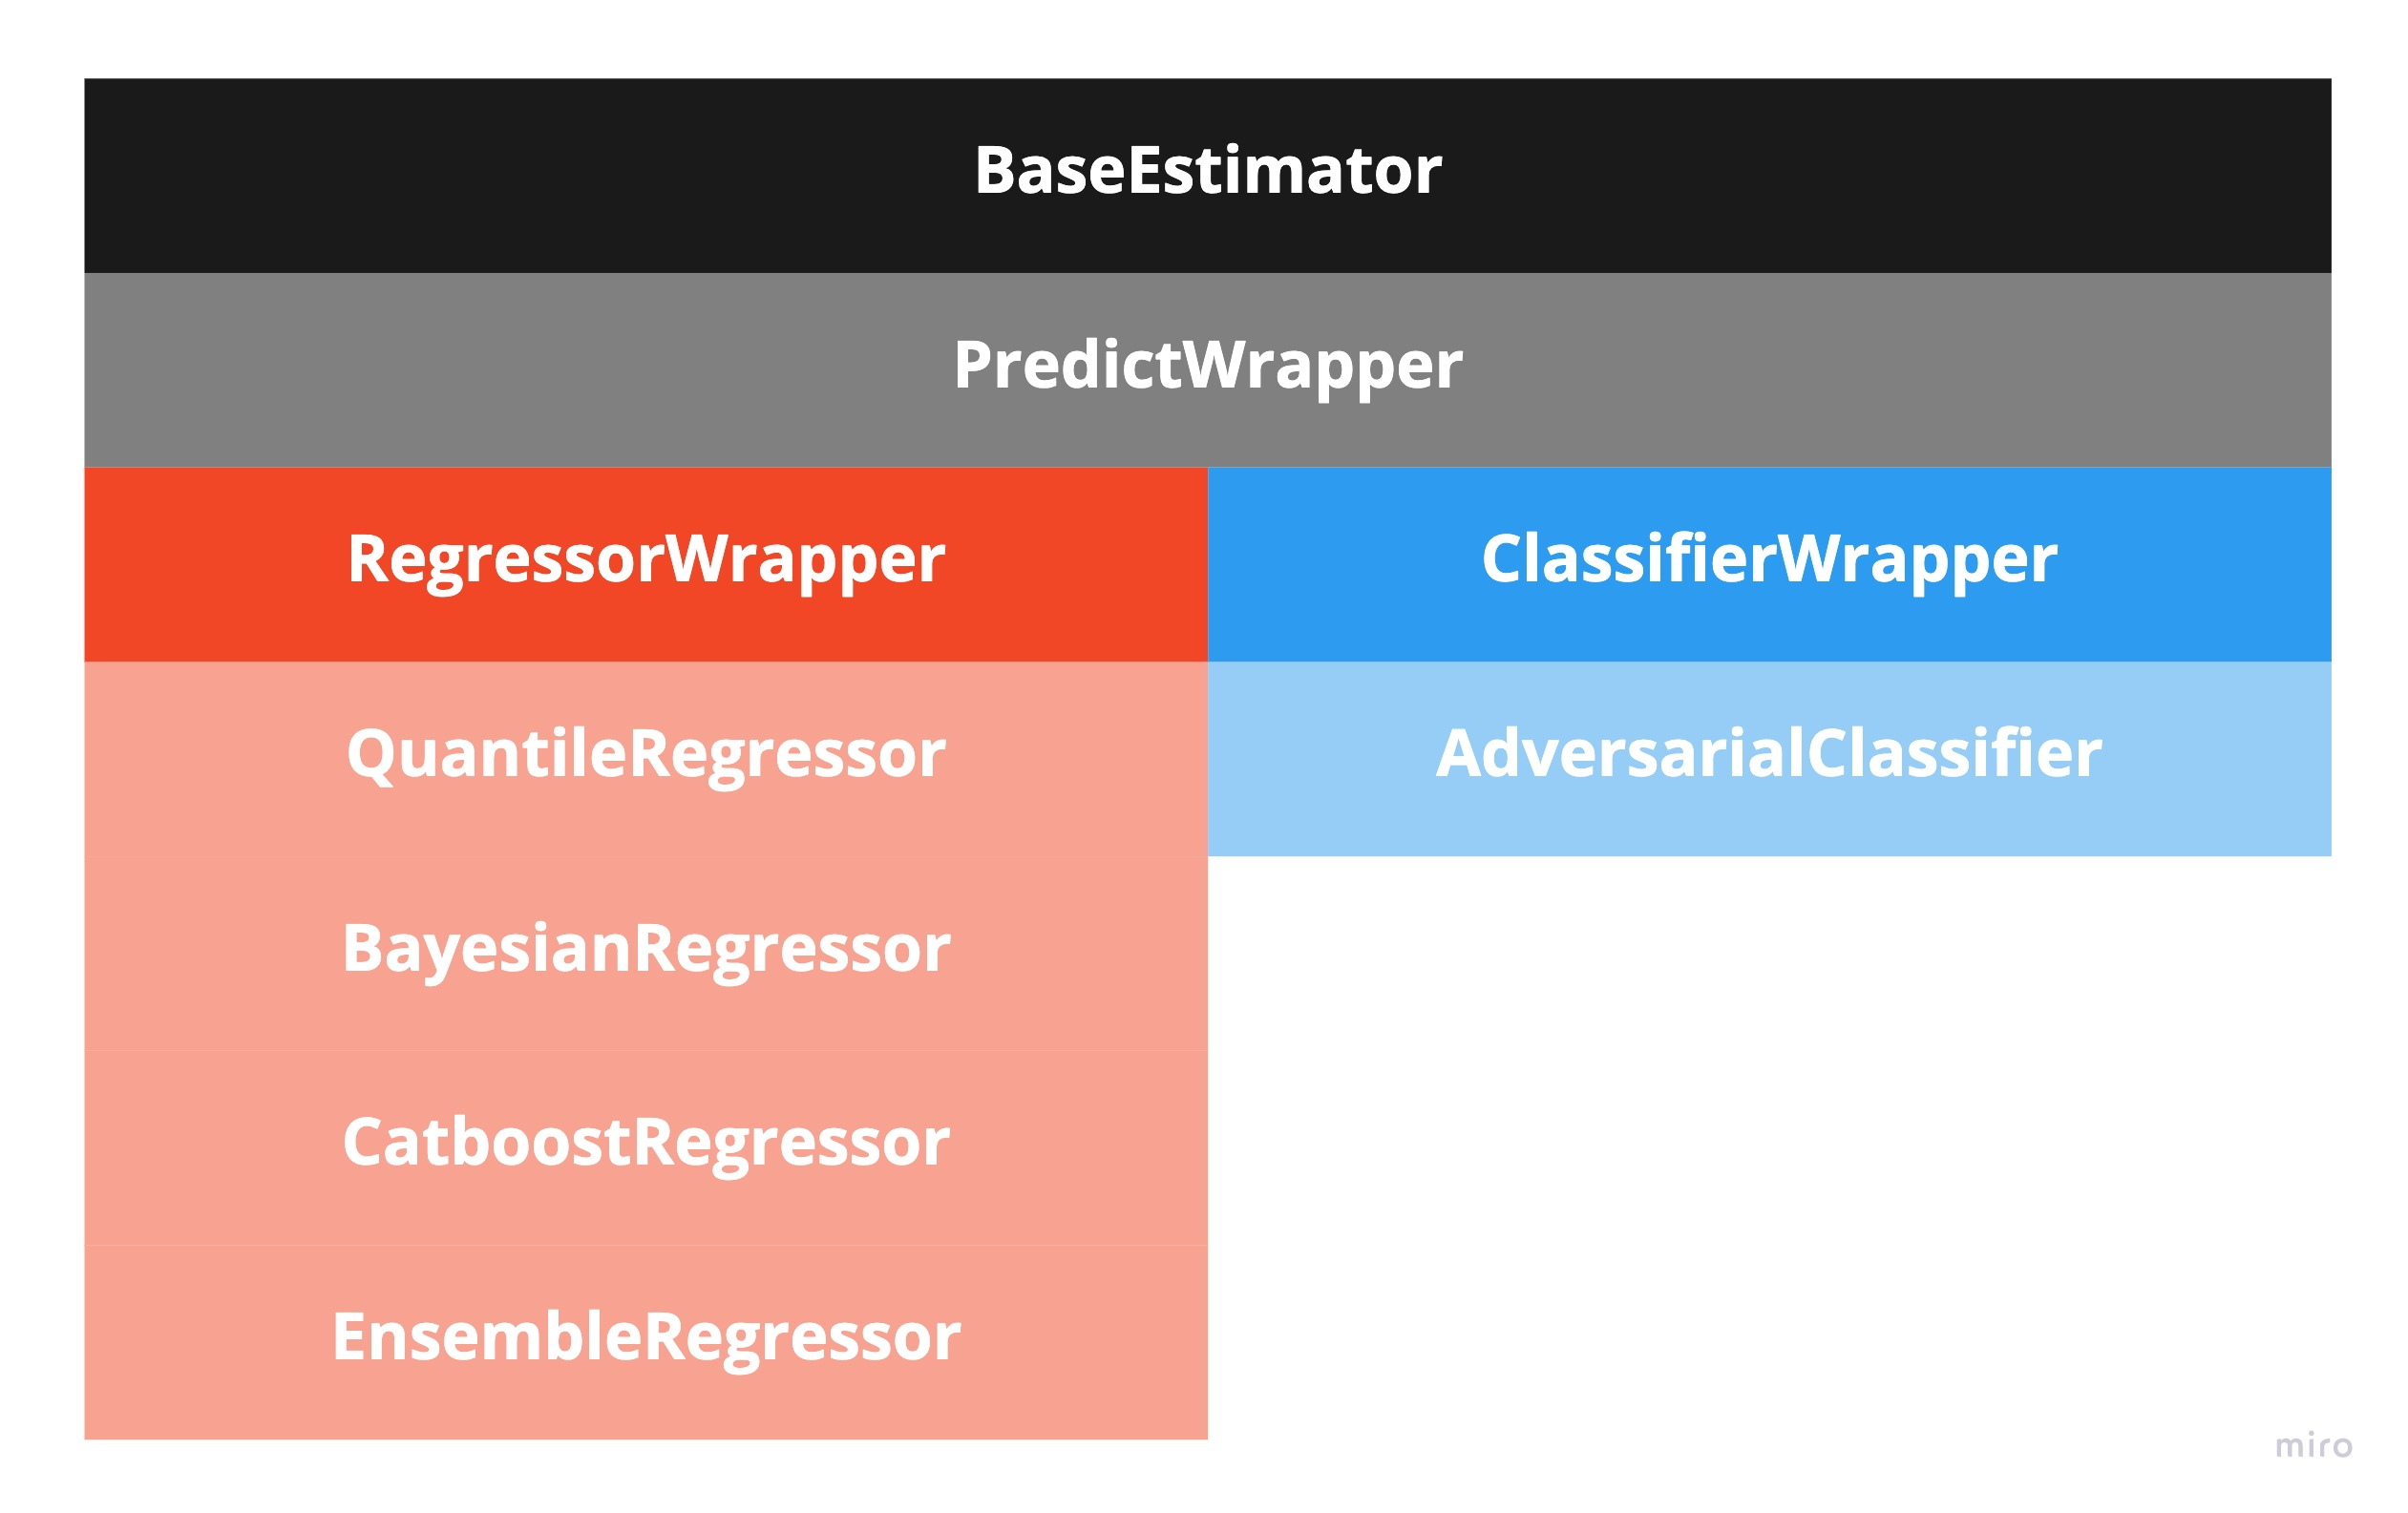
\includegraphics[width=1.15\textwidth]{figures/implementation/class-data-uq.jpg}
         \caption{Data UQ class wrappers.}
         \label{fig:data-uq-class}
     \end{subfigure}
     \hfill
     \begin{subfigure}[b]{0.32\textwidth}
         \centering
         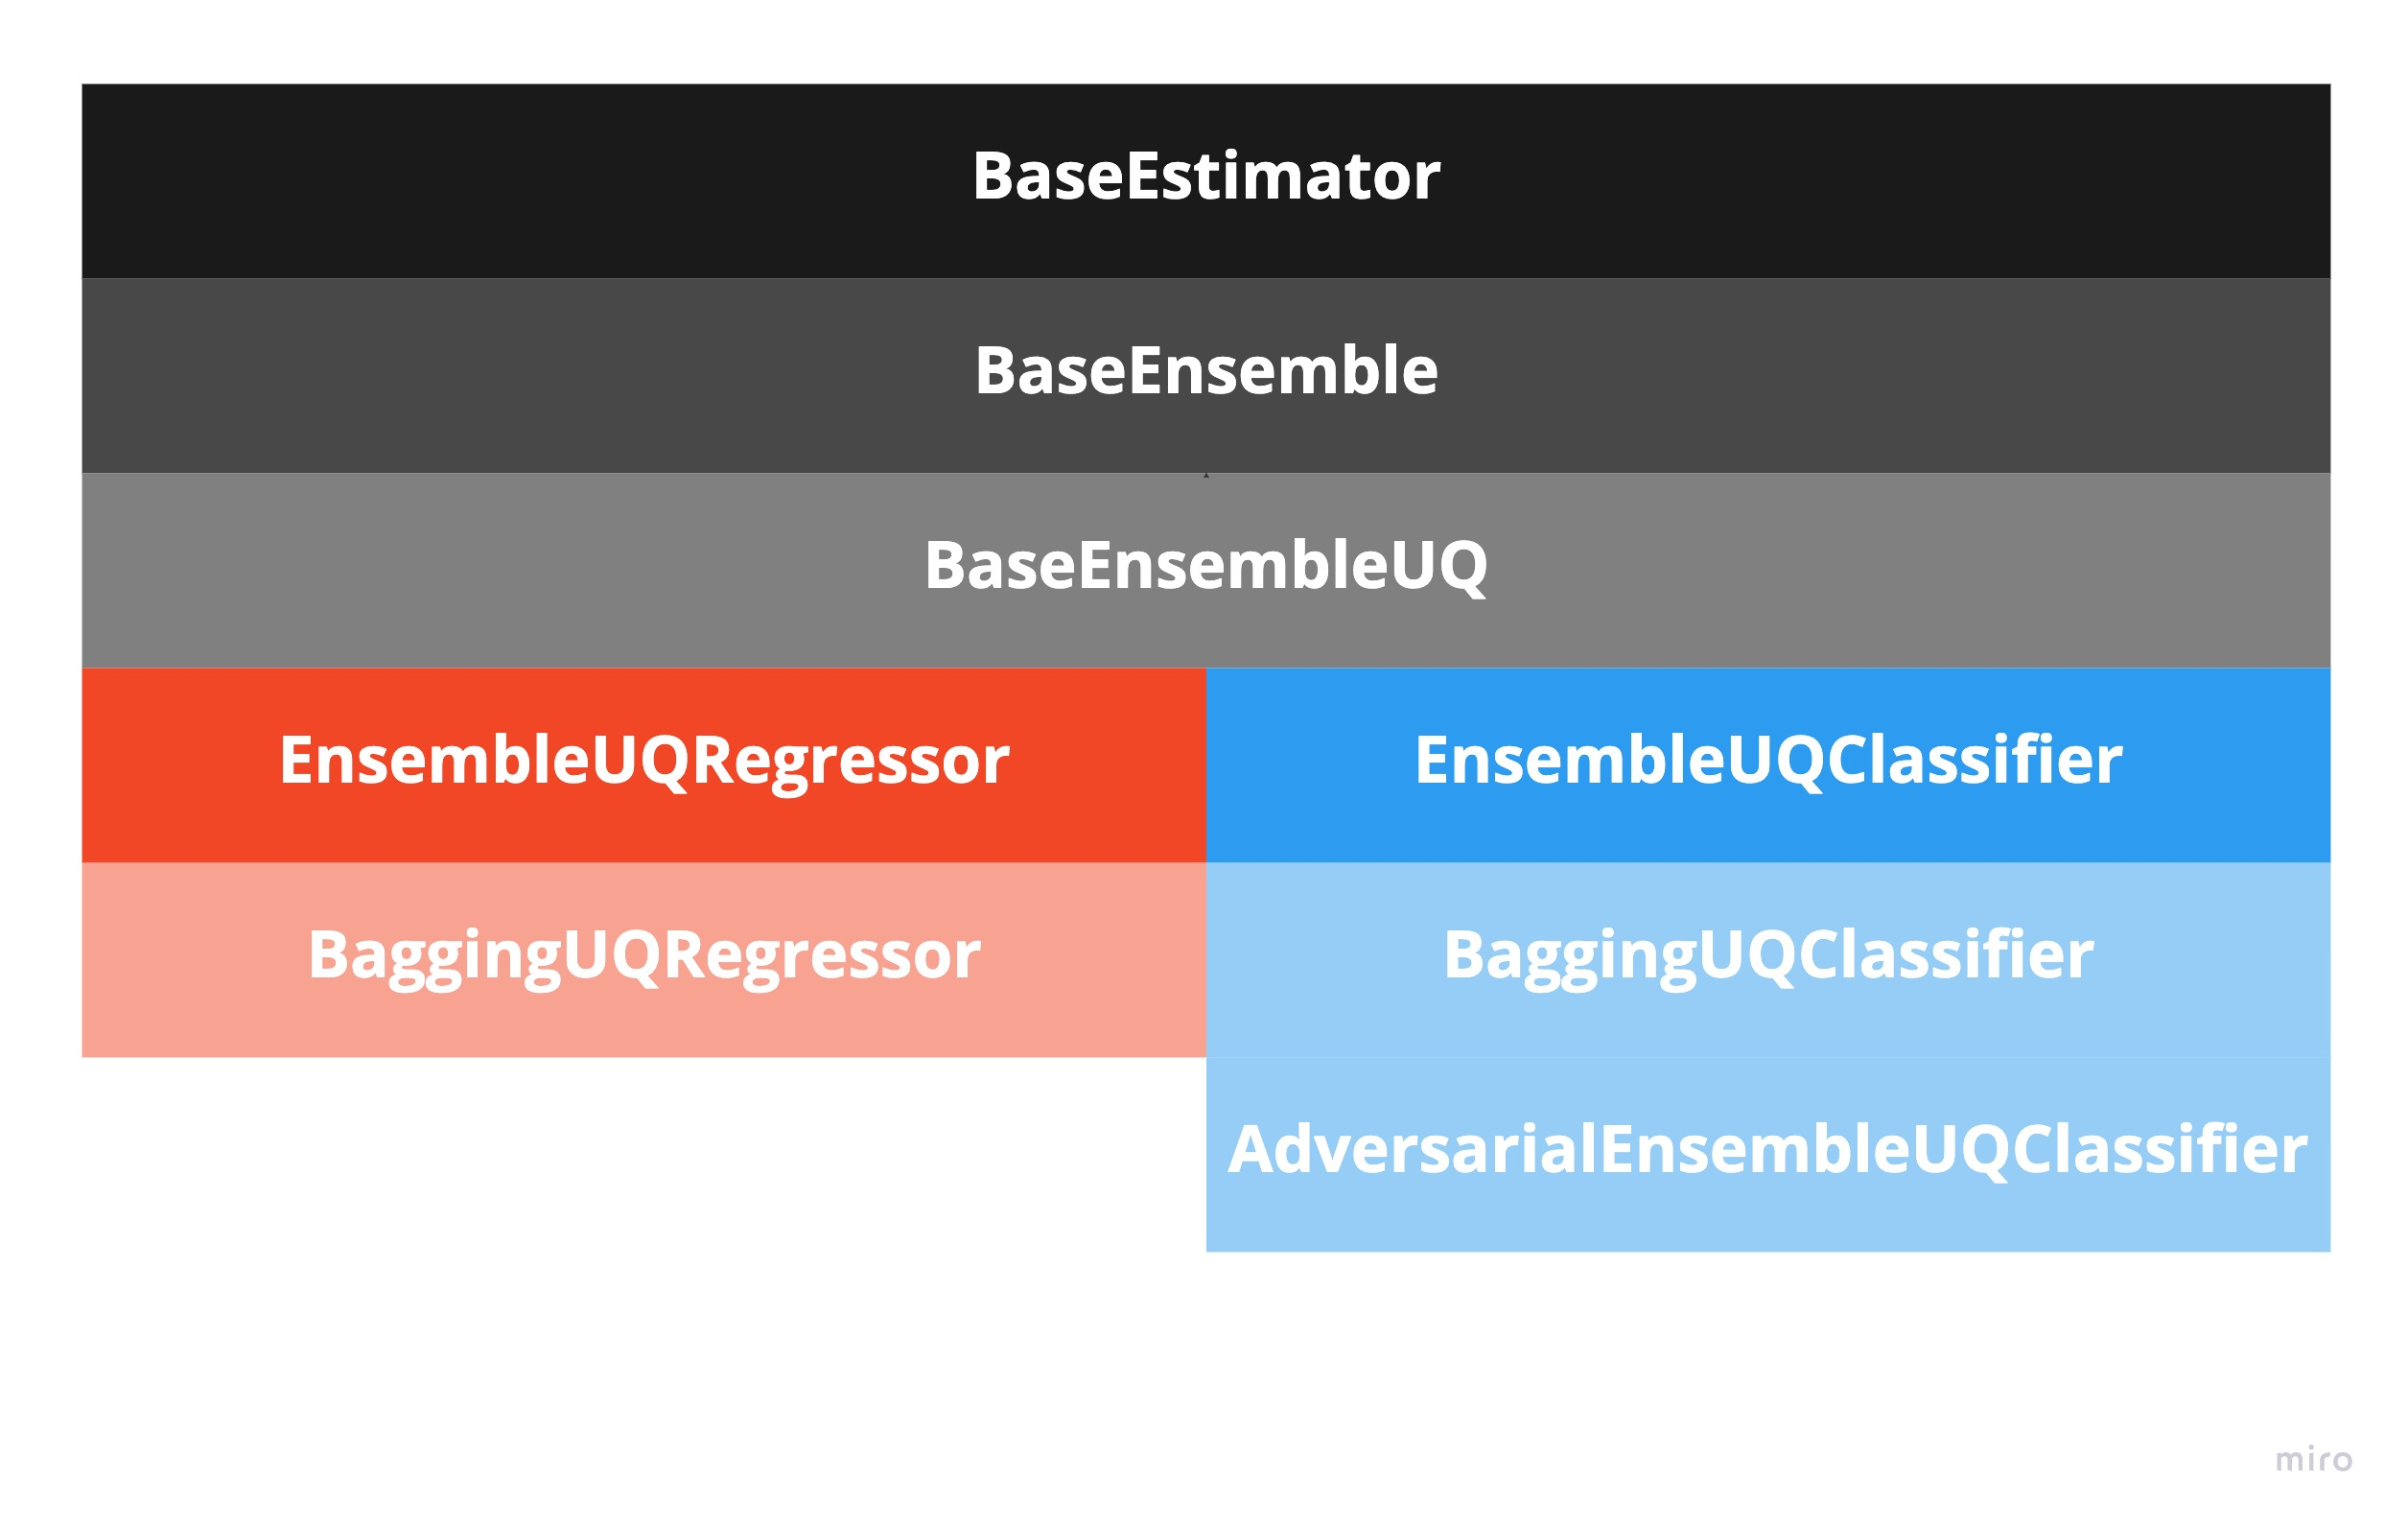
\includegraphics[width=1.15\textwidth]{figures/implementation/class-model-uq.jpg}
         \caption{Model UQ class wrappers.}
         \label{fig:model-uq-class}
     \end{subfigure}
     \hfill
     \begin{subfigure}[b]{0.32\textwidth}
         \centering
         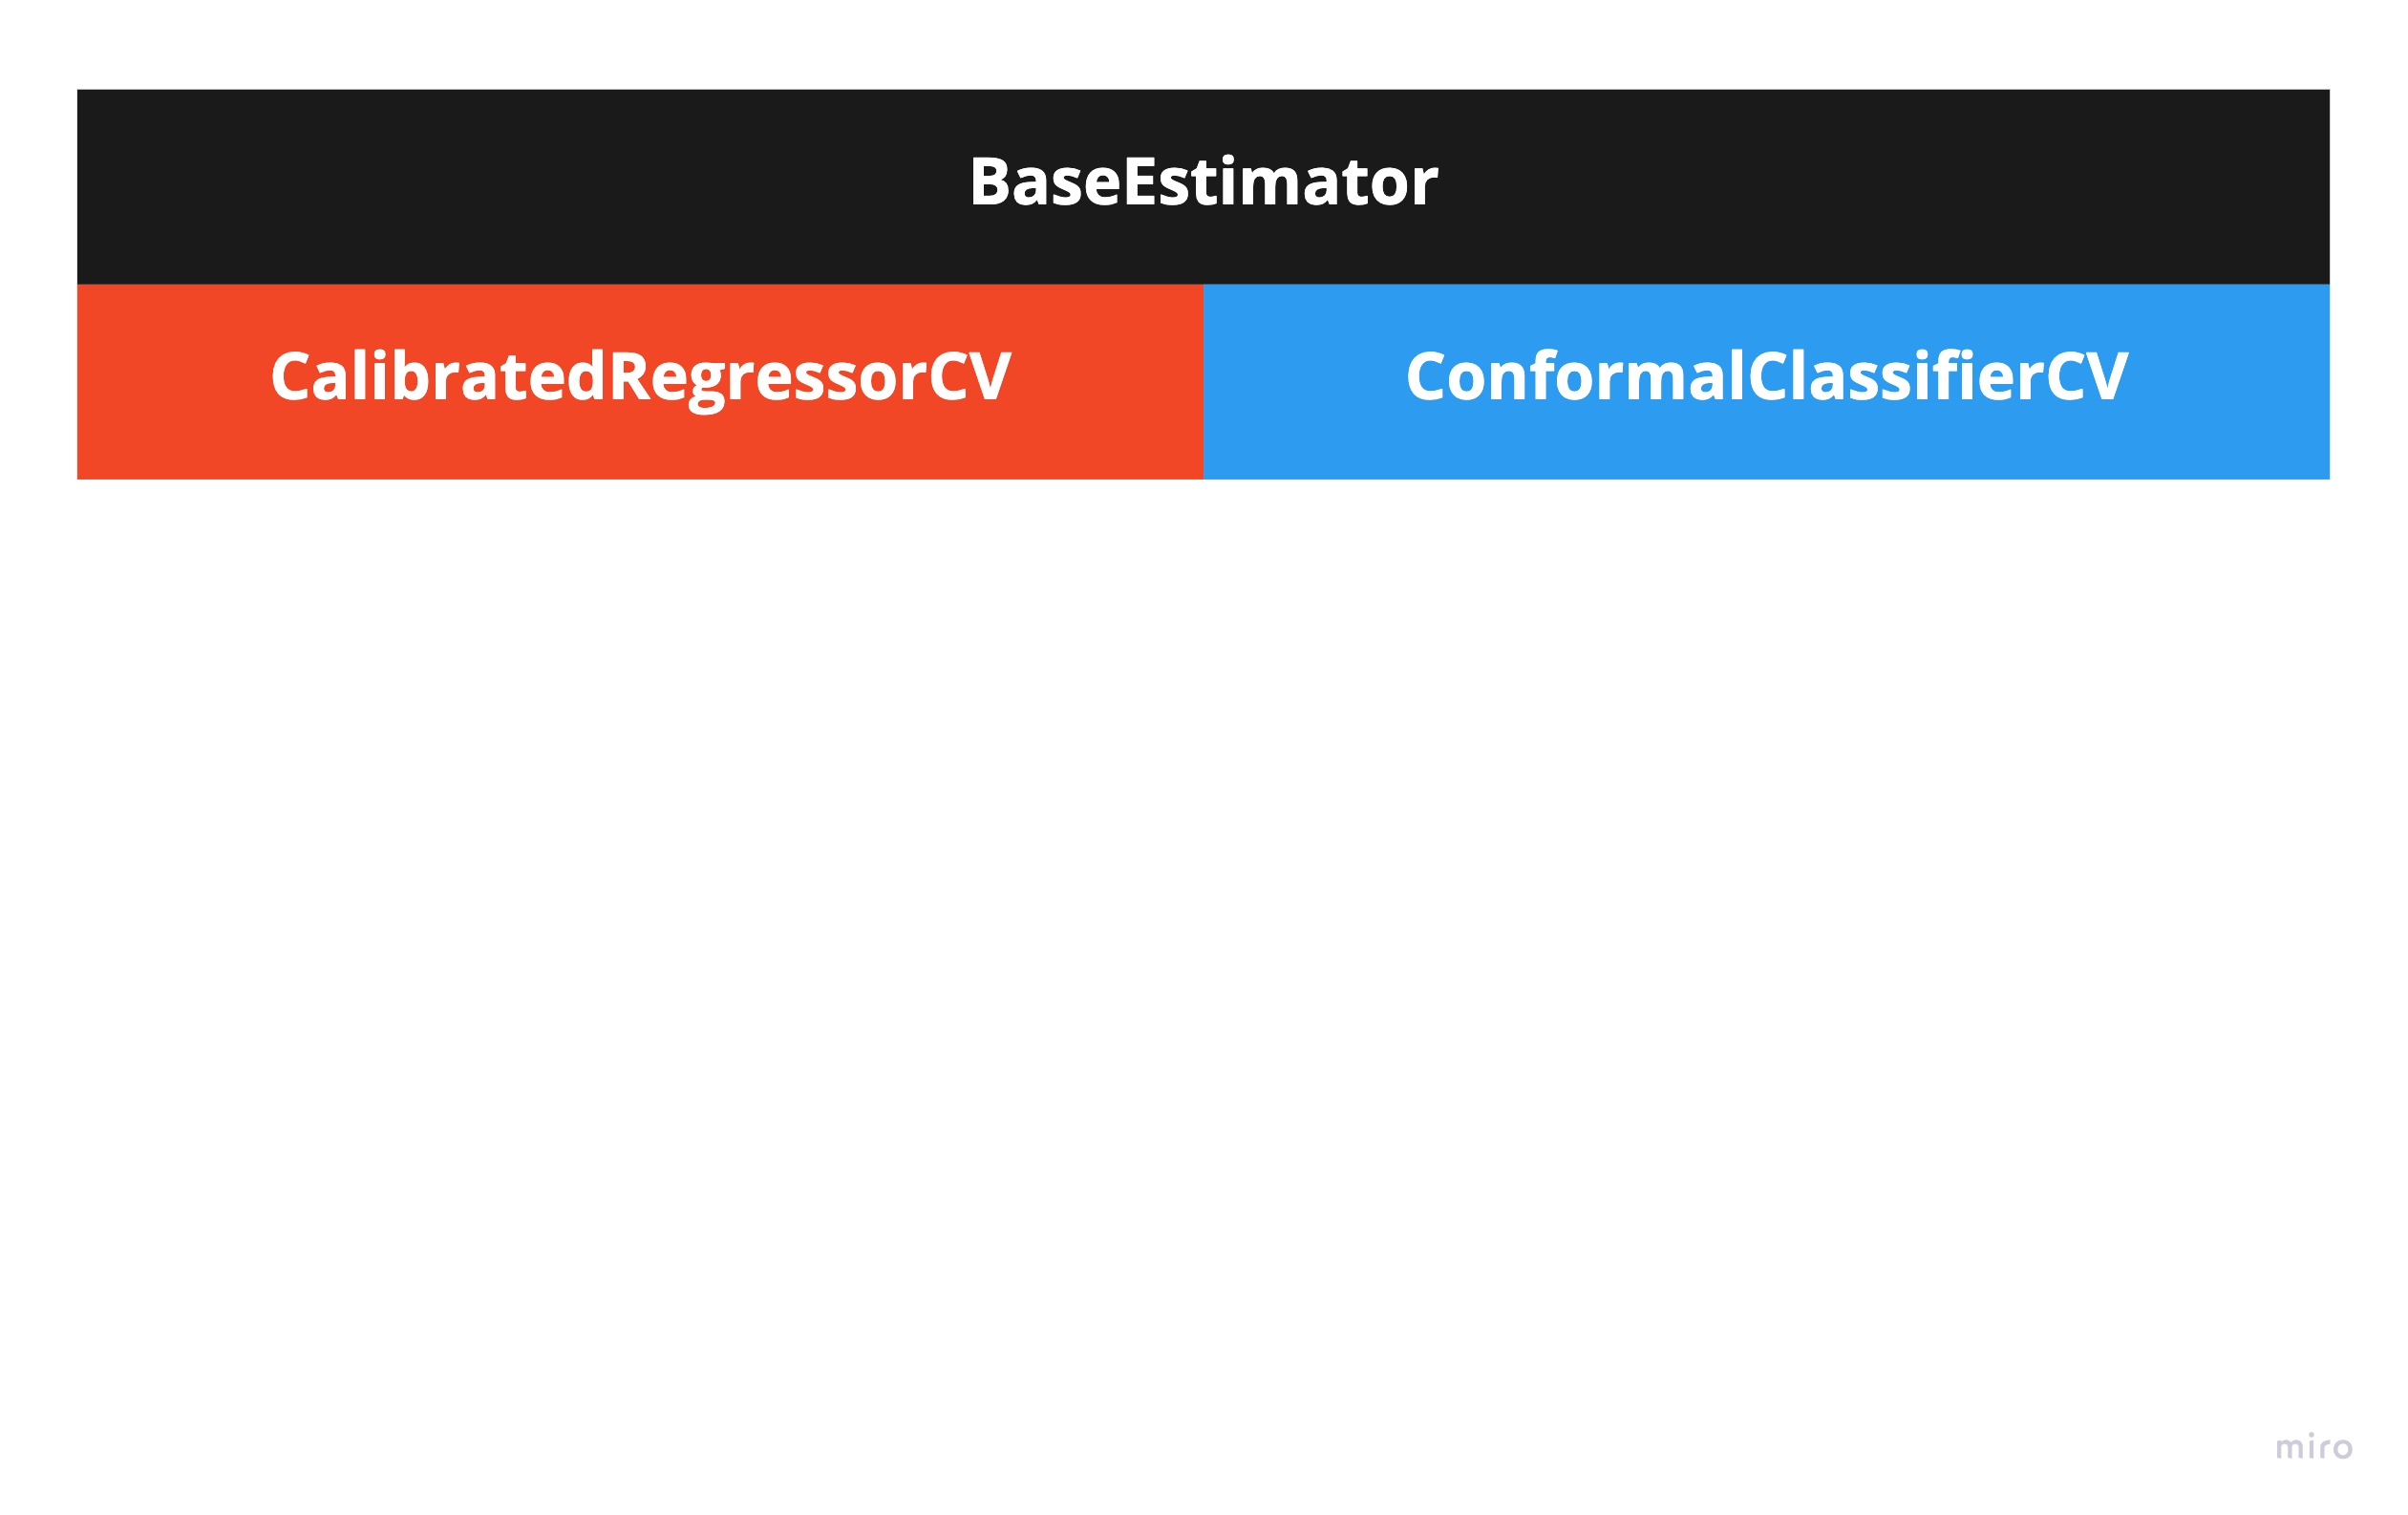
\includegraphics[width=1.15\textwidth]{figures/implementation/class-calibration.jpg}
         \caption{Calibration class wrappers.}
         \label{fig:calibration-uq-class}
     \end{subfigure}
        \caption{Class hierarchy of UQ package. Abstract classes are represented in grey and black. The first black level contains base classes from the \textit{scikit-learn} library. }
        \label{fig:class-hierarchy}
\end{figure}

% Overview of the scikit-learn package




\section{Open-source libraries}

Research and comparison of the different open-source uncertainty quantification tools have been carried out before the development of the package (cf. table \ref{fig:open-source-uq}). 
Most libraries are at a research/development level or are not maintained anymore and cannot be effectively used in production environments. %The Uncertainty Baselines gather metrics, datasets and UQ models for research use. 
We took a step toward simplicity of use and target \textit{scikit-learn} compatibility, which is not offered by any of these libraries except for \textit{Mapie}, \textit{CatBoost} and \textit{UQ360}. However, the first only covers distribution-free models for data UQ, while the second solely focuses on gradient-boosting models. On the other hand, \textit{UQ360} is probably the most similar tool to this work. However, one of our crucial selling points is that any \textit{scikit-learn} compatible model can be turned into a UQ model, which is not the case for \textit{UQ360}. Most of the meta-estimators of our package can exploit intrinsic attributes of models such as Random Forest or Gradient Boosted Trees to perform UQ without the need to provide a calibration dataset. Furthermore, \textit{UQ360} requires more prior uncertainty knowledge to develop UQ models and does not provide adversarial robustness evaluation nor conformal predictions. % unified API classification and regression.

Eventually, the final version of the package harnesses the benefits of these different tools to build a robust and standardised API, e.g. \textit{CatBoost}'s probabilistic learning and virtual ensemble capabilities, \textit{Mapie}'s quantile regression model and some metrics and plots of the \textit{uncertainty toolbox}. In addition, the \href{https://github.com/Trusted-AI/adversarial-robustness-toolbox}{Adversarial Robustness Toolbox (\textit{ART})} was used in the development, in particular their evasion attacks and adversarial training classes. Adversarial UQ wrappers available in the package are based on \textit{ART}. 

Finally, the inclusion of Bayesian learning methods into the package is discussed. After an exploration and testing phase of \textit{PyMC}, \textit{Edward2}, and \textit{PyMC-learn}, it was decided not to include them in this work. \textit{PyMC} and \textit{Edward2} are flexible approaches. Still, they often require manual tuning of prior model distributions and domain expertise to reach a model that is fast to train and accurate. It is, therefore, rather cumbersome to create a simple, \textit{scikit-learn}-like and unified API to train such models without going against the core principles of Bayesian learning. This was the initial objective of the \textit{PyMC-learn} project. However, it is currently left in an unmaintained state and is unusable given our requirements.

% pymc learn 

%- not been updated to the newest major release of PyMC (4.0) 
%Furthermore, as explained in the introductory section \ref{intro:motivation}, there is a clear lack of standardisatisation 



% presents an overview of existing open-source libraries for uncertainty quantification
% Pros and cons
% Why our package is needed.

\begin{table}[htbp]
\centering
\caption{Open-source uncertainty quantification libraries.}
\label{fig:open-source-uq}
\begin{tabular}[t]{p{2.6cm}p{1.4cm}p{1cm}p{1.8cm}p{3.3cm}p{1.5cm}p{2cm}} % 
\toprule
Name & Actor & GitHub stars & Latest release & Focus / Keywords & User friendly & Sk-learn compatible\\
\midrule
Uncertainty Toolbox (\href{https://github.com/uncertainty-toolbox/uncertainty-toolbox}{link}) &---& 1.3k &  Sep. 2021 & metrics, visualisation & high & no\\
Mapie (\href{https://github.com/scikit-learn-contrib/MAPIE}{link}) &---& 500 & Oct. 2022 & metrics, quantile regression, interval estimation  & high & yes\\
CatBoost (\href{https://github.com/catboost/catboost}{link})  &---& 6.9k & Nov. 2022 & gradient-boosted-trees & high & yes\\
UQ 360 (\href{https://github.com/IBM/UQ360}{link} ) & IBM & 176 & --- & General & medium & yes \\
Uncertainty baselines (\href{https://github.com/google/uncertainty-baselines}{link}) & Google & 1k & --- & DL research & low & no\\ 
PyMC (\href{https://github.com/pymc-devs/pymc}{link}) &---& 7.2k & Dec. 2022 & Bayesian learning & low & no\\
Edward2 (\href{https://github.com/google/edward2}{link}) & Google & 619 & --- & Bayesian learning, DL, TensorFlow & low & no\\
PyMC-learn (\href{https://github.com/pymc-learn/pymc-learn}{link}) & --- & 200 & Not maintained & PyMC, sk-learn & high & yes \\
\bottomrule
\end{tabular}
\end{table}%


%%%%%%%%%%%%%%%%%%%%
\chapter{Evaluation}  \label{chatper:evaluation}
%%%%%%%%%%%%%%%%%%%%

%In the evaluation, you convince the reader that your design works as intended. 
%Describe the evaluation setup, the designed experiments, and how the
% experiments showcase the individual points you want to prove.

% This section is usually 5-10 pages.



\section{Data} \label{section:datasets}
Models described in section \ref{design:uq-models} and \ref{design:UQ-models-G2T} are trained and evaluated on the following datasets.

\subsection{General uncertainty quantification}

\begin{itemize}
    \item The \href{https://www.cs.toronto.edu/~delve/data/boston/bostonDetail.html}{Boston housing dataset} contains information related to housing in the Boston area and the median value of a home is to be predicted (regression task). It was originally collected by the U.S Census Service and comprises roughly 500 cases.
    \item The \href{https://archive.ics.uci.edu/ml/datasets/breast+cancer+wisconsin+(diagnostic)}{breast cancer dataset} is a well-known binary classification dataset to detect cancer in a breast mass. The ten available features correspond to different measurements of cell nucleus (radius, texture, smoothness, etc.). It is composed of 569 data points.
    %\item The event scoring this dataset is an Oracle proprietary binary classification dataset of 55k events. The task is to predict whether or not specific financial events are fraudulent or suspicious using 30 features. This is a strongly imbalanced dataset as only 2\% of the cases are labelled fraudulent. 
\end{itemize}

\subsection{Graph-to-text}
\begin{itemize}
    \item \href{https://webnlg-challenge.loria.fr/challenge_2020/}{WebNLG dataset}: open-source dataset consisting of thousands of knowledge graphs representing facts, along with their corresponding textual representation describing these facts in natural language.
    \item SAR: Oracle proprietary dataset consisting of around 100 suspicious financial activity reports and manually associated knowledge graphs.
    \item The synthetic datasets for token-level hallucination defined in section \ref{design:synthetic-hallucination-data}. They are based on WebNLG and SAR datasets.
\end{itemize}

\begin{table}
    \centering
        \caption{Descriptive statistics for the graph-to-text datasets.}
    \label{table:G2T-datasets-descriptive-stats}
    \begin{tabular}{rrrrrrrr}
\toprule
&  & \multicolumn{3}{c}{Text length} & \multicolumn{3}{c}{Nb. of edges per graph}  \\
    \cmidrule(rl){3-5} \cmidrule(rl){6-8} 
 Dataset &count&         min & mean & max &         min  & mean & max \\
\midrule
WebNLG  & 16095 & 19  &  114.8  & 444 &    1 & 2.9 & 7  \\
SAR      & 105 &  1723 &  2443.0 &  4203 &  20 &  35.3 &  80  \\
\bottomrule
\end{tabular}
\end{table}
%\subsubsection{Synthetic Data Creation for token-level hallucination detection}

\section{Metrics for uncertainty quantification}


There are several metrics to consider when evaluating an uncertainty quantification model. Calibration and negative log-likelihood are the usual candidates. However, task-specific metrics are sometimes available and often provide more insights into the UQ quality.

\subsection{Regression} \label{metrics:regression}

Uncertainty quantification models for regression are usually used to provide confidence bounds around predictions. Proper bounds should be as tight as possible while still maintaining the $\alpha$ coverage property $\Pb( \hat l_i \leq y_i \leq \hat h_i) \geq 1 - \alpha$. This observation leads to the introduction of two metrics: the mean prediction interval width  $MPIW = \frac{1}{n} \sum_i \hat h_i - \hat l_i$ and the prediction interval coverage probability, or coverage score, $PICP = \frac{1}{n} \sum_i I\left\{\hat l_i \leq  y_i \leq \hat h_i\right\}$. The latter can be turned into a metric that should be minimised using the coverage absolute error: $CAE = \mid PICP - \alpha \mid$. The trade-off between $MPIW$ and $PICP$ is illustrated in figure \ref{fig:example-uq-regression-metrics}. Other metrics, such as sharpness or adversarial group calibration, are sometimes used to evaluate regression UQ models. 


\begin{figure}
     \centering
     \begin{subfigure}[b]{0.49\textwidth}
         \centering
         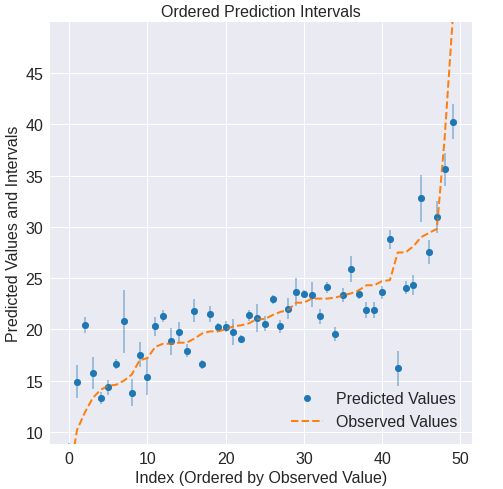
\includegraphics[width=\linewidth]{figures/eval/metrics/example_reg_metric_1.png}
         \caption{Underconfident predictions with $MPIW = 2.20$ and $PICP = 0.31$.}
     \end{subfigure}
     \hfill
     \begin{subfigure}[b]{0.49\textwidth}
         \centering
         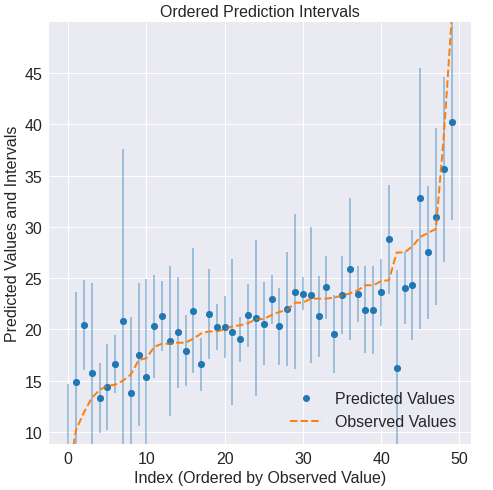
\includegraphics[width=\textwidth]{figures/eval/metrics/example_reg_metric_2.png}
         \caption{Calibrated predictions with $MPIW = 12.18$ and $PICP = 0.87$.}
     \end{subfigure}

        \caption{Example of the trade-off between the $MPIW$ and $PICP$ UQ metrics for regression.}
        \label{fig:example-uq-regression-metrics}
\end{figure}

\subsection{Classification}

Uncertainty quantification models for classification are usually evaluated using one of the following metrics:
\begin{itemize}
    \item Expected calibration error (ECE). It corresponds to the miscalibration area, i.e. the area between the reliability curve and the diagonal line in reliability plots. Given a set of exclusive data bins $\{B_l\}_l$ covering the calibration set $\bigcup_i B_l = X_{cal}$,  the ECE can be computed as follows. The lower the score, the better the calibration and, therefore, the quality of uncertainty quantification.
    $
    ECE = \sum_l \frac{|B_l|}{n} \mid acc(B_l) - conf(B_l)\mid
    $
    \item Brior score: another calibration metric, i.e. the equivalent of mean square error for predicted probabilities:
    $
    BS = \frac{1}{N} \sum_i {(p_{i,1} - y_i)^2} 
    $
    \item Oracle collaborative accuracy, f1 score, etc.\cite{collaborativeUQMetrics2021}. They measure the performance of the uncertainty quantification system under the capacity constraints of an oracle (e.g. human moderator). A given fraction of the testing dataset is forwarded to an oracle which returns the correct labels without errors. Only the most uncertain data points are selected to be labelled by the oracle: $D^{U}_\alpha = \{(x_i,y_i) \;:\: u_i = U(f, x_i) >= q_{1-\alpha} \}$ where $q_{1-\alpha}$ is the $1-\alpha$ quantile of the uncertainty scores series $\{u_i\}_i$. Given a scoring metric $M$, e.g. accuracy, the associated oracle collaborative metric $OC^M_{\alpha}$ is defined as
    $$
        OC^M_{\alpha} = (1 - \alpha) \cdot M(D \setminus D^U_\alpha) + \alpha 
    $$
    Intuitively, the better the uncertainty quantification, the more likely it is for $D^U_\alpha$ to contain prediction errors. The oracle collaborative accuracy is illustrated in figure \ref{fig:example-uq-classification-metrics}.
    \item Coverage checks for conformal predictions models\cite{conformalPredictions2021}: the equivalent of regression coverage metrics for classification, e.g. $\frac{1}{n} \sum_i I\{y_i \in C(x_i)\} \geq 1 - \alpha$
\end{itemize}


\begin{figure}
     \centering    
     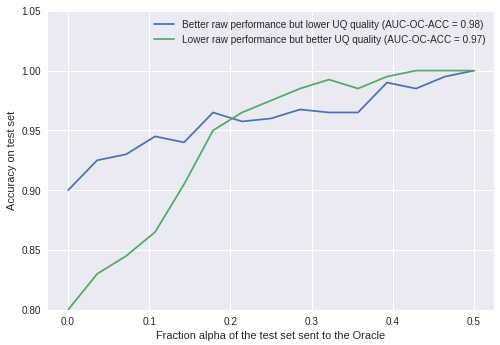
\includegraphics[width=0.67\textwidth]{figures/eval/metrics/oracle_collab_acc.png}
     \caption{Example of the evolution of the collaborative accuracy metric for two models as a function of $\alpha$. The \textit{green} model has a lower default accuracy but is better calibrated. At $\alpha=20\%$, it outperforms the \textit{blue} one.}
     \label{fig:example-uq-classification-metrics}
    
\end{figure}

The oracle-family of metrics is best suited for applications where humans are available for the labelling operation\cite{collaborativeUQMetrics2021}. However, in this work, it is used as a tool to assess the quality of uncertainty quantification models, which are uncoupled with the idea of oracle query ratio (or entropy threshold). To remove this dependence, we argue that the area under the oracle collaborative accuracy curve, i.e. $AUC-OC^{ACC}$,  is better suited to compare UQ models. Furthermore, this metric can be used during model selection to produce not only performing models but also calibrated ones. Indeed, if two models have a comparable accuracy score, the $AUC-OC^{ACC}$ metric favours the better-calibrated one.



\subsection{Factual uncertainty evaluation for graph-to-text} \label{factual-uq-metrics}

Classification UQ models are usually evaluated using metrics such as ECE or oracle collaborative accuracy. However, they are not particularly well-suited for text generation since multiple textual outputs are typically considered correct predictions. Furthermore, the oracle collaborative family of metrics are most relevant in an environment where the model can ask a human for help when it is uncertain about a prediction. In text generation, that is not very effective because humans have to intervene for each predicted token. For instance, a paragraph consisting of 50 words could require 5-10 manual checks, one per uncertain token, which is infeasible in practice, especially for many paragraphs.
Moreover,  LM calibration is often evaluated using downstream classification tasks (e.g. paraphrase detection), which is not relevant for the graph-to-text use case.
% factual point
Finally, none of these metrics can provide insights into the factuality of the model. Indeed, they are more focused on evaluating the uncertainty of the language model, which is less relevant to end-users than factual uncertainty. This also occurs with metrics such as BLEU, ROUGE or perplexity.

We propose to evaluate UQ models using factuality-aware metrics, i.e. reward models producing a high uncertainty score whenever a hallucination is generated. Given a hallucination entropy dataset $\Tilde{D} = \{(t_i, a_i, h_i)\}_{i=1}^N$ where $t_i \in V$ represent tokens, $a_i \in \{0,1\}$ hallucinations labels and $h_i$ the entropy for the token prediction $t_i$, we define the mean hallucination entropy (MHE) and the mean hallucination entropy difference $MHED$ as:

$$
MHE = \frac{ \sum_i a_i h_i }{\sum_i a_i}
$$

$$
MHED = \frac{\sum_i a_i h_i}{\sum_i a_i} -   \frac{ \sum_i \neg a_i h_i}{\sum_i \neg a_i}
$$


$\Tilde{D}$ can either be constructed synthetically via the procedure defined in section \ref{design:synthetic-hallucination-data} or via the hallucination detection models of section \ref{design:hallucination-detection-models}. These proposed metrics depend on the factuality of the model itself. In this work, it is evaluated using \textit{faithfulness}, which is defined as one minus the mean hallucination ratio\cite{factualityEnhancedLM} ($r_H$), i.e. the ratio between the number of hallucination entities to the total number of entities in the text:

$$
r_h(G,T) = \frac{ |HALLU_{NE}|}{|ALL_{NE(T)}|} = \frac{1 }{q}  \sum_{i=1}^q I\{NE(T)_i \not \in NE(G) \} \;\text{such that}\; q = |ALL_{NE(T)}|
$$
 Additionally, a variation of $r_H$, specialised on number-like tokens, is defined. It is referred to as the number hallucination or $r_h^{num}$. For the latter, $ALL_{NE(T)}$ is not computed using spaCy's default NER model but rather using the \textit{like\_num} property of tokens in spaCy (cf. \href{https://spacy.io/api/token}{documentation}).

%%%%%%%%%%%%%%%%%%%%
\chapter{Experiments}
%%%%%%%%%%%%%%%%%%%%

\section{Demonstration of the UQ package workflow}

This section is a concrete example of how one can use the uncertainty quantification package to improve the quality of the models trained iteratively. Consider a base model for regression trained by the user for which he/she cares about reliable UQ. In this case, it is represented by a CatBoost regression GBT and reaches an R2 of 0.74:

\begin{lstlisting}[language=Python, caption=Base user model.]
def get_base_model():
    return CatBoostRegressor(...)
model = get_base_model()
model.fit(X_train, y_train)
\end{lstlisting}

The first step of the workflow is to use one of the uncertainty wrappers. It is assumed that the user is interested in both data and model uncertainty via a size-5 seed ensemble.

\begin{lstlisting}[language=Python, caption=Step 1: train UQ model.]
from uqlearn.data_uq import DataUQWrapper
from uqlearn.model_uq import ModelUQWrapper

uq_model = ModelUQWrapper(
    DataUQWrapper(model), ensemble='seed', n_estimators=5
)
uq_model.fit(X_train, y_train)
preds, std = uq_model.predict(X_test, return_std=True)
\end{lstlisting}

The updated UQ model can also predict standard deviations. The results are displayed, e.g. via confidence intervals, for the first 5 test data points in figure \ref{fig:demo-viz}. Model uncertainty, which can be viewed as the spread of the x-axis in the top-left plot,  seems to play a notable role in this example, especially for data point 2. In fact, the mean prediction is far from the true value, as highlighted in the bottom-right plot. Overall, the reliability diagram of the model and the ordered prediction intervals can be found in figure \ref{fig:demo-calibration}. The case of data point 2 is not isolated, and most of the predicted confidence intervals are too narrow, which results in a very over-confident and uncalibrated model (miscalibration area of 0.37).

\begin{figure}[!ht]
    \centering
    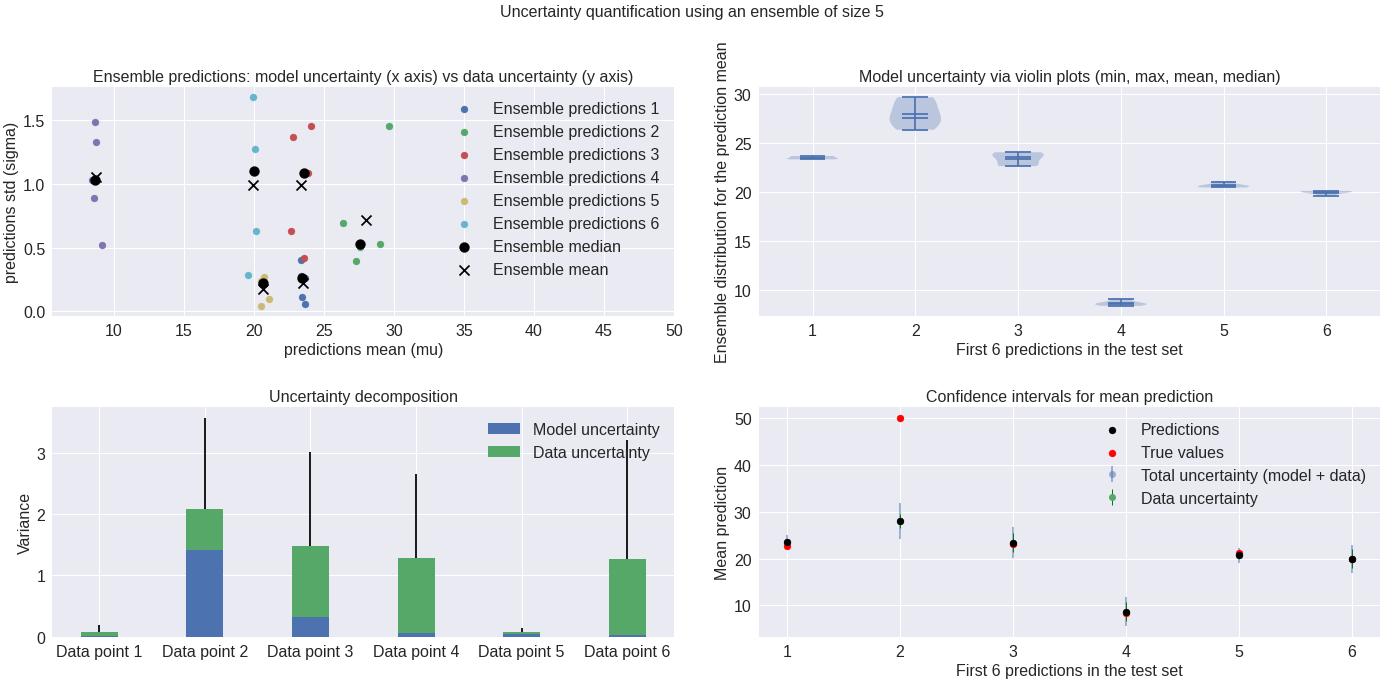
\includegraphics[width=\linewidth]{figures/eval/demo/demo_eval.png}
    \caption{Demo. Evaluation of the first 5 test data points. The top-left plot contains the raw predictions for each member of the ensemble. The bottom-left one highlights how total uncertainty is distributed across its data and model components. Different variations of confidence internals are shared in the two right figures.}
    \label{fig:demo-viz}
\end{figure}

\begin{figure}[!ht]
    \centering
    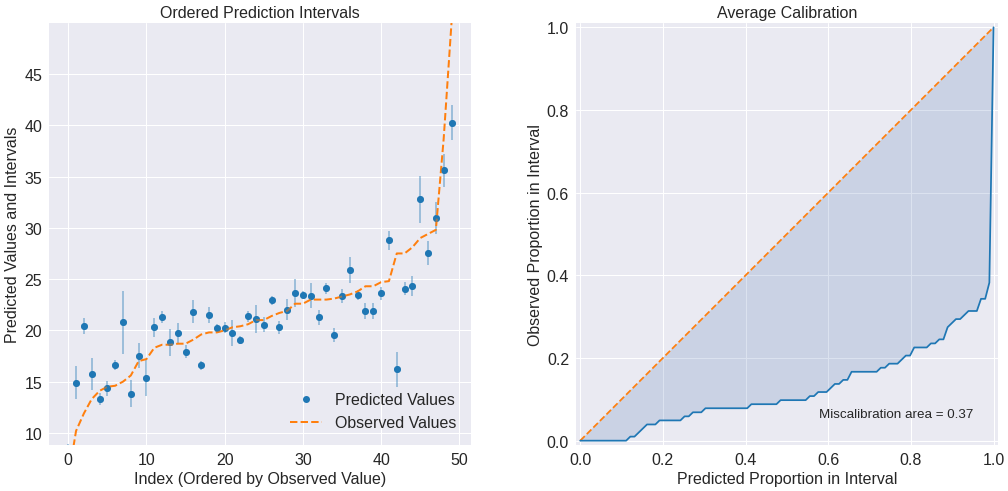
\includegraphics[scale=0.40]{figures/eval/demo/4_evaluation.png}
    \caption{Demo. Reliability plots for the UQ model.}
    \label{fig:demo-calibration}
\end{figure}

The package also offers calibration tools to address this issue. It is the second step of this workflow. The \textit{calibrated\_uq\_model} is better calibrated (cf. figure \ref{fig:demo-recalibration}) and can be trusted regarding uncertainty quantification. The evaluation metrics described in section \ref{metrics:regression} are reported in table \ref{tab:demo:metrics} for both models. 

\begin{lstlisting}[language=Python, caption=Step 2: calibration of UQ model.]
from uqlearn.calibration import CalibratedRegressorCV

calibrated_uq_model = CalibratedRegressorCV(uq_model, cv=4)
calibrated_uq_model.fit(X_train, y_train)
preds, std = calibrated_uq_model.predict(X_test, return_std=True)
\end{lstlisting}


\begin{figure}[h!]
    \centering
    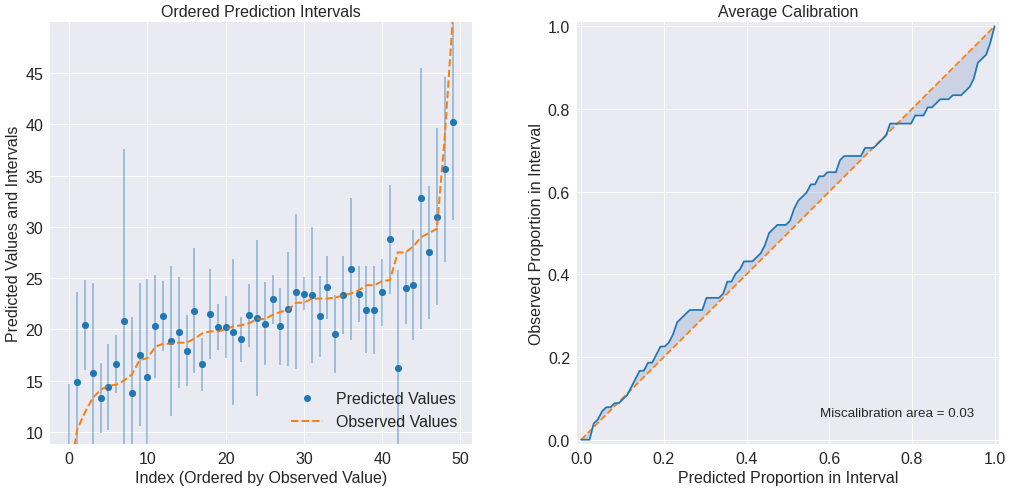
\includegraphics[scale=0.40]{figures/eval/demo/6_calibration_evaluation.png}
    \caption{Demo. Reliability plots for the calibrated UQ model.}
    \label{fig:demo-recalibration}
\end{figure}



\begin{table}[h!]
    \centering
    \begin{tabular}{lrr}
    \toprule
    Metric & Base value & Value after calibration \\
    \midrule
       R2 & 0.74 & 0.74\\
       Coverage score &	0.25 & 0.93 \\
 %      Coverage absolute error & 0.70 & 0.02\\
 %      Width score	& 1.92 & 13.64\\
       NLL &	42.71  & 2.15\\
       Miscalibration area & 0.38 & 0.06 \\
    \bottomrule
    \end{tabular}
    \caption{Demo. Regression UQ evaluation metrics for uncalibrated and calibrated models.}
    \label{tab:demo:metrics}
\end{table}

\section{UQ validity checks}

In this experiment, different UQ models are compared on a regression and a classification dataset: seed, bagging and hyper-parameter ensembles of different sizes, i.e. 10, 20, 30 and 50 members. The models are not re-calibrated using an extra calibration dataset. 



% show plots and example outputs
\subsection{Regression}

Gaussian Process, Random Forest, Gradient-Boosted Trees, Ridge regression, and Bayesian Ridge Regression models are trained on the Boston Housing dataset and evaluated using the following metrics: R2, Miscalibration area ($ECE$), coverage absolute error and Negative Log-Likelihood (NLL). All metrics are independently computed for total, data, and model uncertainties. Besides, data uncertainty is further estimated via an intrinsic and an extrinsic UQ model. The extrinsic model is a quantile regression model trained using cross-validation. %to produce calibration sets. 

\begin{figure}[!ht]
    \centering
    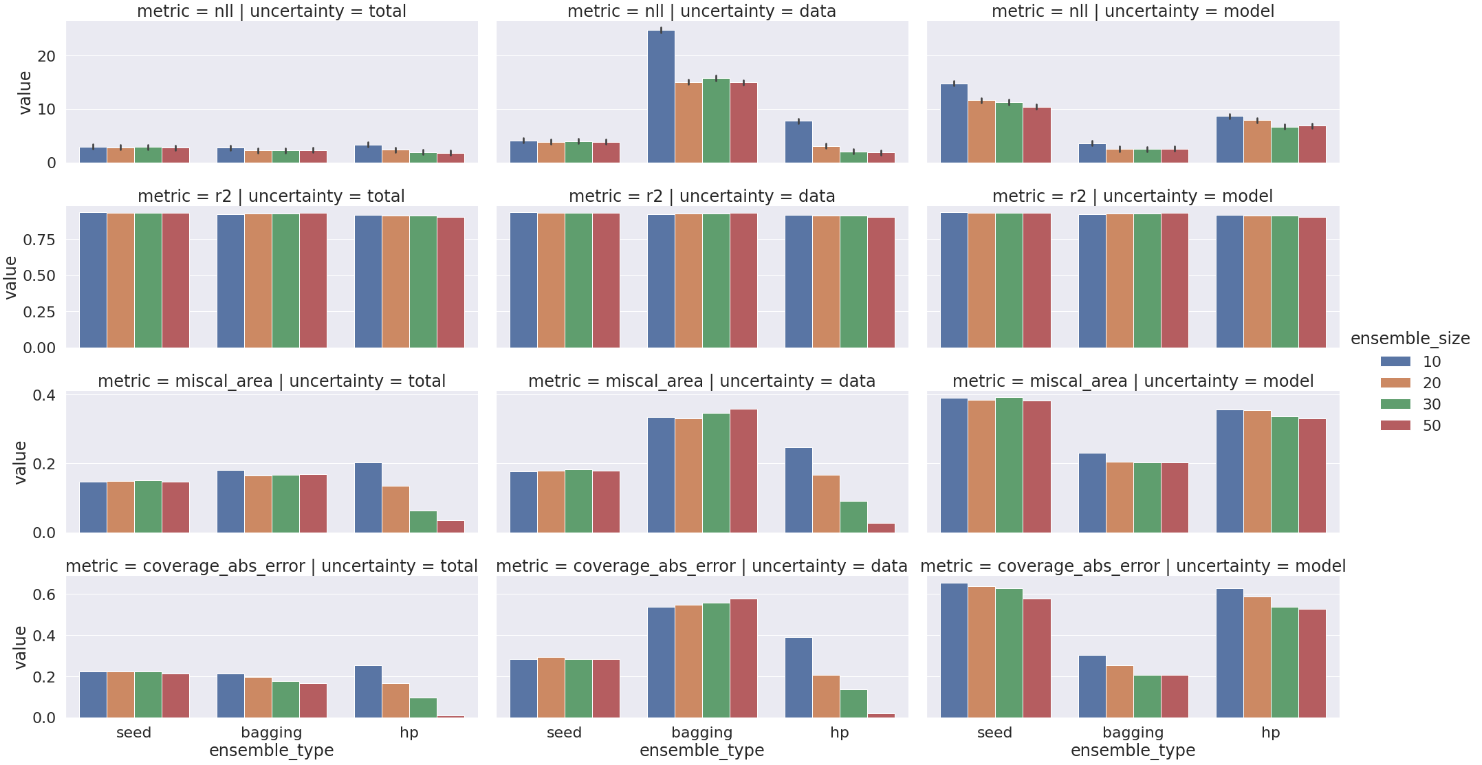
\includegraphics[width=\linewidth]{figures/eval/uqlearn/regression-results.png}
    \caption{Results of regression experiment for CatBoost model.}
    \label{fig:regression-catboost-results}
\end{figure}
Given the large amount of data collected and the size constraints of this thesis, the detailed analysis in figures \ref{fig:regression-catboost-results} and \ref{fig:regression-catboost-heatmap} is only performed for a single base model type: a CatBoost Gradient-Boosted tree. It has been chosen due to the versatility of results. Nevertheless, a summary of the top-performing models trained is shared in figure \ref{fig:regression-best-models}. 

\begin{figure}[!htbp]
    \centering
    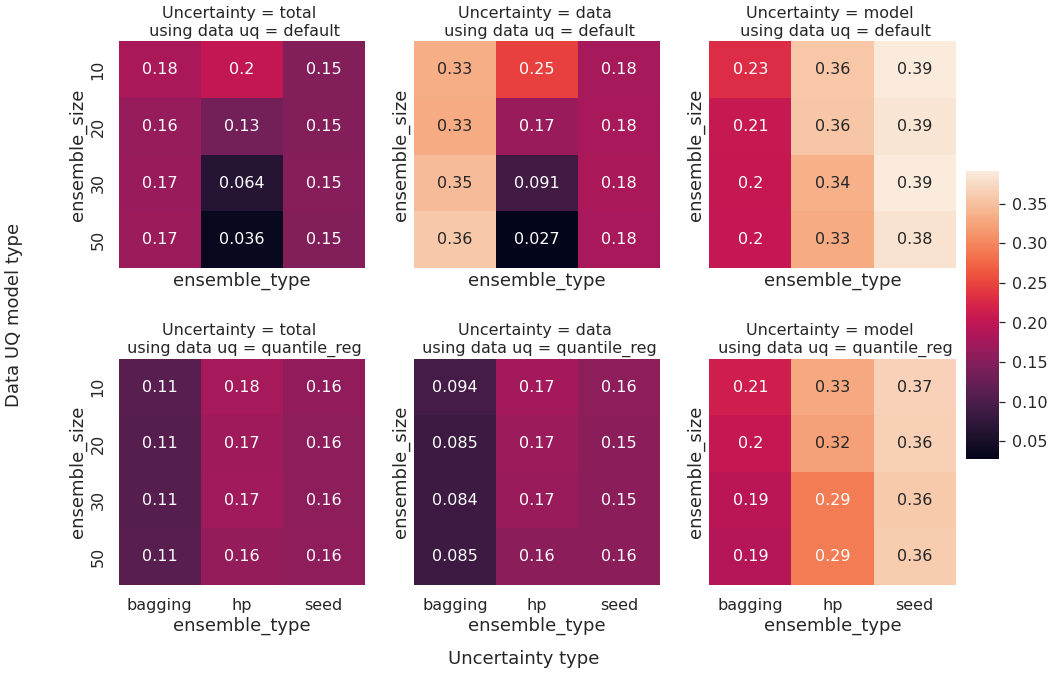
\includegraphics[width=0.95\linewidth]{figures/eval/uqlearn/regression-catboost-heatmap.png}
    \caption{Miscalibration area for different uncertainty types and data UQ models.}
    \label{fig:regression-catboost-heatmap}
\end{figure}

In figure \ref{fig:regression-catboost-results}, we observe that in terms of mean prediction performance, all CatBoost models are comparable with $0.89 \leq R2 \leq 0.93$. However, regarding UQ performance, disparities are present across models, and the hyper-parameter ensembles of size 50 appear to outmatch all other models. A larger ensemble size also has a positive impact on UQ performance for all metrics. Furthermore, model uncertainty systematically underperforms compared to total or data uncertainty. This can be further examined in figure \ref{fig:regression-catboost-heatmap} that highlights miscalibration scores for all different models in a heat map. The latter plot also allows us to investigate the performance divergence between intrinsic and extrinsic uncertainty models. In particular, quantile regression coupled with bagging or seed ensemble produces superior UQ models than their intrinsic counterparts. However, the intrinsic hyperparameter 50-ensemble eventually constitutes the best model with a miscalibration area of 0.027.

\begin{figure}[!htbp]
    \centering
    \begin{subfigure}[b]{0.99\textwidth}
         \centering
         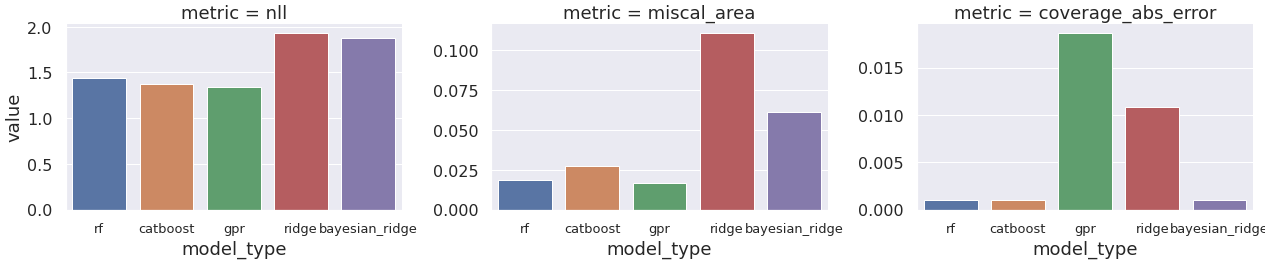
\includegraphics[width=\textwidth]{figures/eval/uqlearn/regression-best-models.png}
         \caption{Metrics scores for the best models.}
         \label{fig:regression-best-models-metrics}
     \end{subfigure}
     \hfill
     \begin{subfigure}[b]{0.99\textwidth}
         \centering
         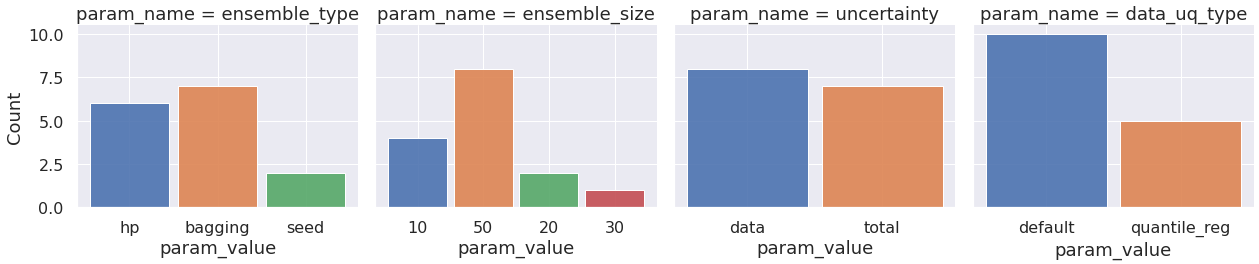
\includegraphics[width=\linewidth]{figures/eval/uqlearn/regression_param_hist.png}
         \caption{Distribution of the best hyperparameters. }
         \label{fig:regression-hyperparam-hist}
     \end{subfigure}
     \caption{Summary plots for the best regression estimators.}
     \label{fig:regression-best-models}
\end{figure}


An equivalent analysis can be conducted for all different base model types. A summary of the best UQ models for each metric is displayed in figure \ref{fig:regression-best-models-metrics}. Random Forest, GBT and Gaussian Process are similar in terms of performance and outperform both Ridge and Bayesian Ridge regression models. In figure \ref{fig:regression-hyperparam-hist}, the distribution of the hyperparameters leading to these best models is plotted. Overall, intrinsic data UQ, coupled with large size (e.g. 50) hyper-parameter or bagging UQ ensembles, give rise to decent UQ models for the Boston Housing dataset. 


\subsection{Classification}


A similar analysis is conducted for classification models. However, no distinction is made between total, data and model uncertainty because most evaluation metrics are solely based on class probabilities. In contrast with entropy, the latter cannot be decomposed into different uncertainty parts. This allows us to study the performance of different models in a single plot as shared in figure \ref{fig:classification-results}. As it was already the case on the regression dataset, in terms of F1 score, all models are comparable. However, the uncertainty quantification metrics inform us that ensemble size has a weaker impact on performance compared to the regression case. Furthermore, GBT usually leads to the best UQ models, as shown in figure \ref{fig:classification-best-models}.



% no difference between data and model uncertainty because the metrics used only consider probabilities and not entropies 

\begin{figure}[!htbp]
    \centering
    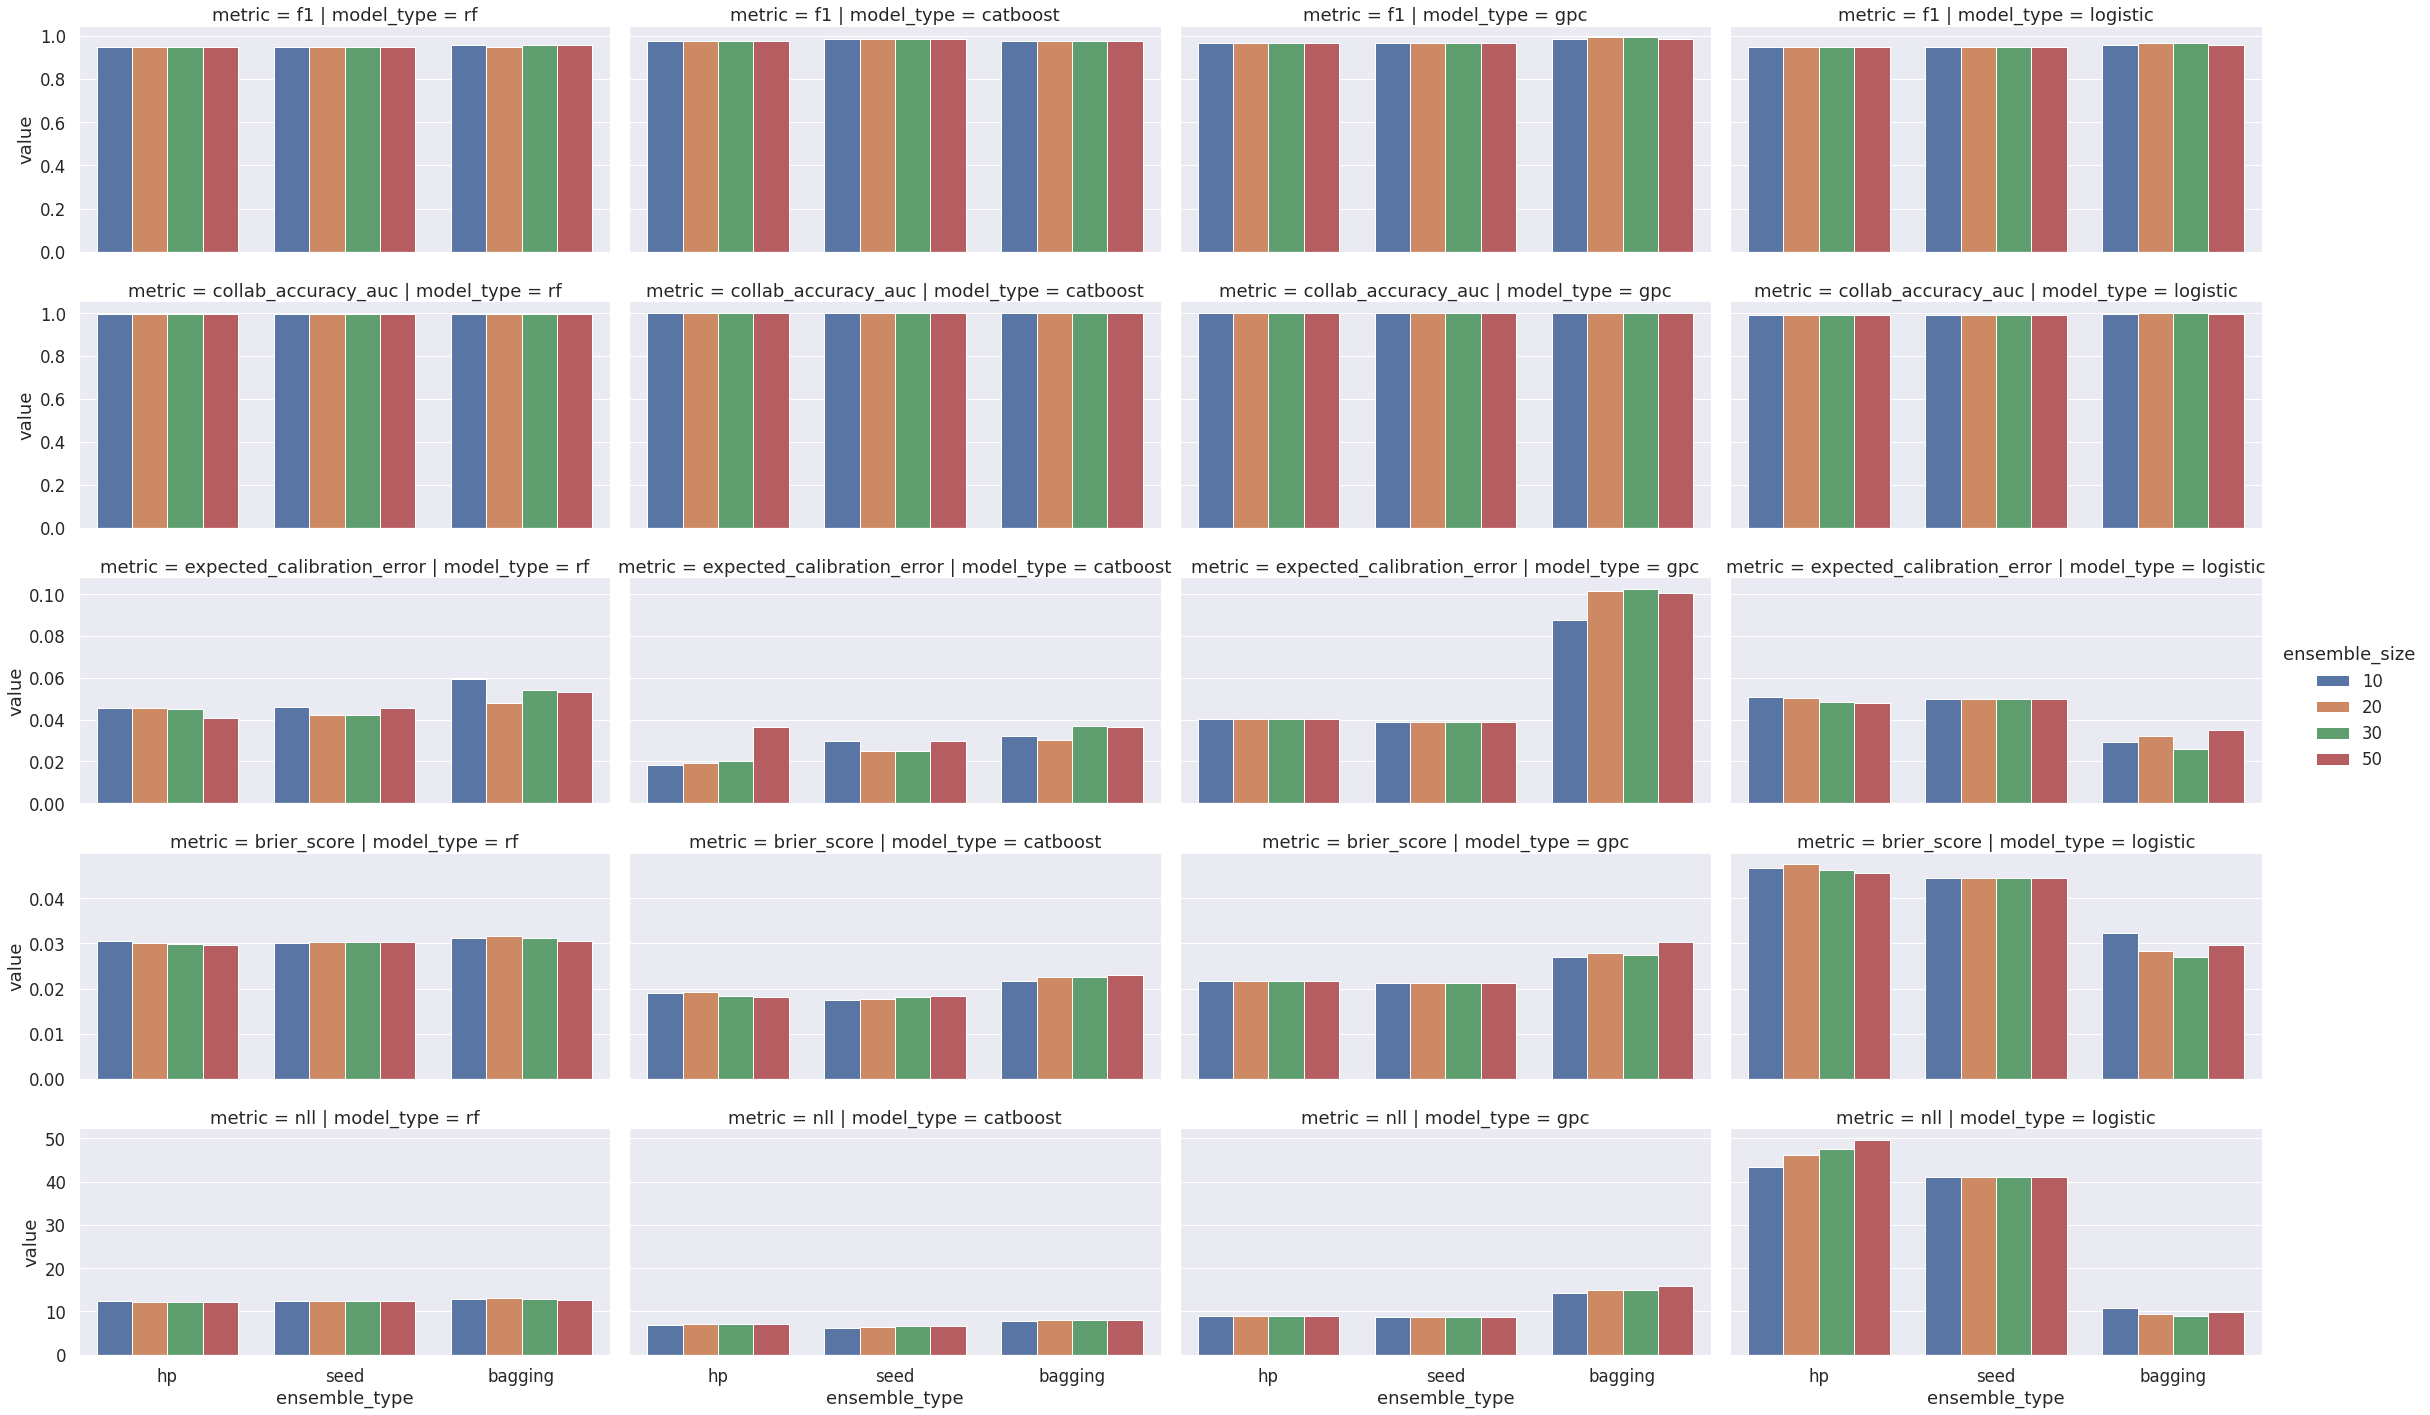
\includegraphics[width=1.1\linewidth]{figures/eval/uqlearn/classification-results.png}
    \caption{Results of classification experiment.}
    \label{fig:classification-results}
\end{figure}

\begin{figure}[!htbp]
    \centering
    \begin{subfigure}[b]{0.99\textwidth}
         \centering
         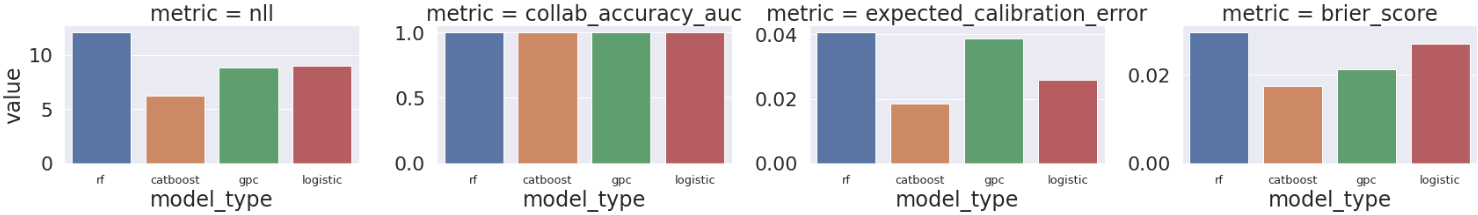
\includegraphics[width=\textwidth]{figures/eval/uqlearn/classification-best-models.png}
         \caption{Metrics scores for the best models.}
         \label{fig:classification-best-models-metrics}
     \end{subfigure}
     \hfill
     \begin{subfigure}[b]{0.99\textwidth}
         \centering
         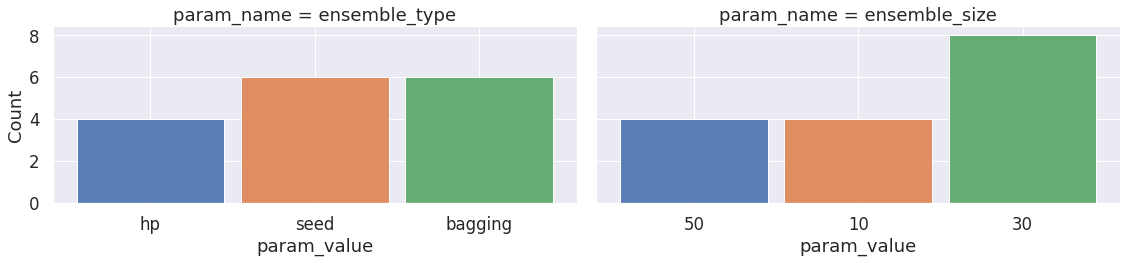
\includegraphics[width=\linewidth]{figures/eval/uqlearn/classification-param-hist.png}
         \caption{Distribution of the best hyperparameters. }
         \label{fig:classification-hyperparam-hist}
     \end{subfigure}
     \caption{Summary plots for the best classification estimators.}
         \label{fig:classification-best-models}
\end{figure}


%TODO
%\subsection{Clustering}


\section{Out-of-distribution evaluation} \label{experiment:OOD-evaluation}

In the previous section, the evaluation of UQ models was focused on in-distribution data. Indeed, the test set was constructed from the same underlying distribution as the training data. However, in production environments, out-of-distribution (OOD) examples are frequent, and it is important to be able to rely on the output of UQ models in these scenarios, especially if the performance of the model drops.
%might drop significantly when evaluated on these special data points. 
\newpage
In the benchmark datasets described in section \ref{section:datasets}, no extra OOD test set is available to perform such an evaluation. Consequently, it is first required to generate these OOD data points. Different types of perturbations $\delta$ with intensity $\epsilon$ for a given dataset $D_{test} = (X,Y) =\{(x_i,y_i)\}_{i=1}^N$ are considered:

\begin{itemize}
    \item White noise perturbations: $\delta = \epsilon \cdot \Normal(0, Var(X))$
    \item Fast-Gradient-Sign Perturbations\cite{FGSM} (FGSM): $\delta = \epsilon \cdot Sign\left(\nabla_X \Loss(f(X), Y)\right)$
    \item Uncertainty-Driven Perturbations\cite{UDP} (UDP): $\delta = \epsilon \cdot Sign\left(\nabla_X \Entropy(f(X)) \right)$
\end{itemize}

The OOD test set is defined as $D_{OOD} = (X + \delta, Y)$. In figure \ref{fig:adversarial-evaluation}, the evolution of the accuracy, the calibration error and the mean entropy over the OOD test predictions are displayed as functions of the attack step size $\epsilon$ for a Logistic Regression model on the breast cancer dataset. The model seems to be relatively robust against white noise attacks. The fast-gradient-sign perturbations are more harmful since the accuracy drops below the $50\%$ threshold with a step size of $0.15$. However, although the model makes more mistakes, it is also more confident about its predictions. This indicates a failure of the model to evaluate its uncertainty on OOD data. Indeed, the $ECE$ increases significantly, and after a short growth phase (i.e. $\epsilon < 0.1)$, the mean entropy quickly reaches the minimum level.
% ensembling does provide a better performance 
% idea metric: the area below current max curve; if the curve is strictly increasing, it is 0.
\begin{figure}
    \centering
    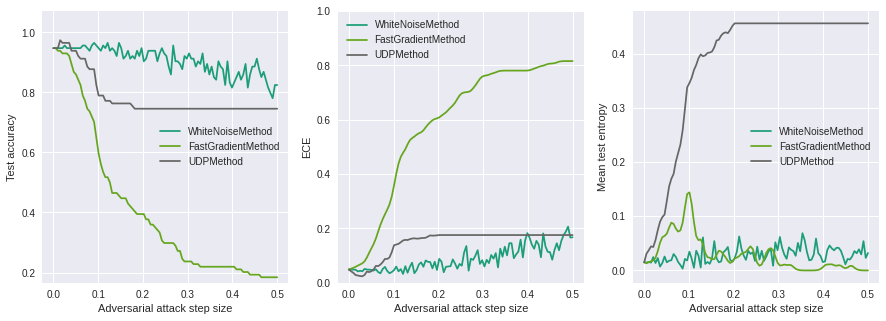
\includegraphics[width=\linewidth]{figures/eval/eval_adv_uq.png}
    \caption{Adversarial evaluation of a Logistic Regression model (breast cancer dataset).}
    %The robustness of the model is tested against three different attack types.
    \label{fig:adversarial-evaluation}
\end{figure}

\begin{figure}[!htbp]
    \begin{subfigure}{\textwidth}
      \centering
      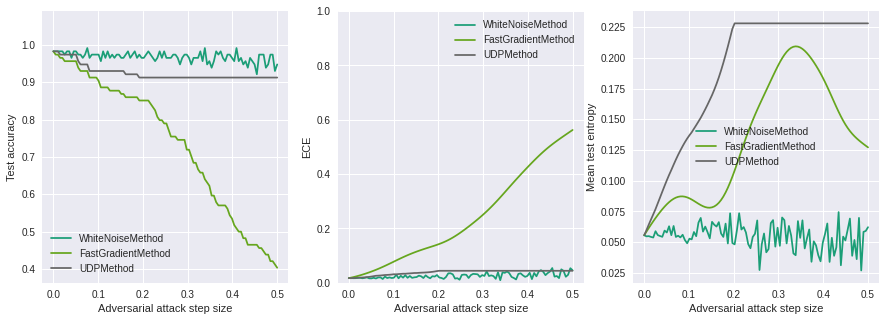
\includegraphics[width=\linewidth]{figures/eval/eval_adv_uq_train_noise.png}
      \caption{Adversarial training on the white noise attack.}
    \end{subfigure}
     \begin{subfigure}{\textwidth}
      \centering
      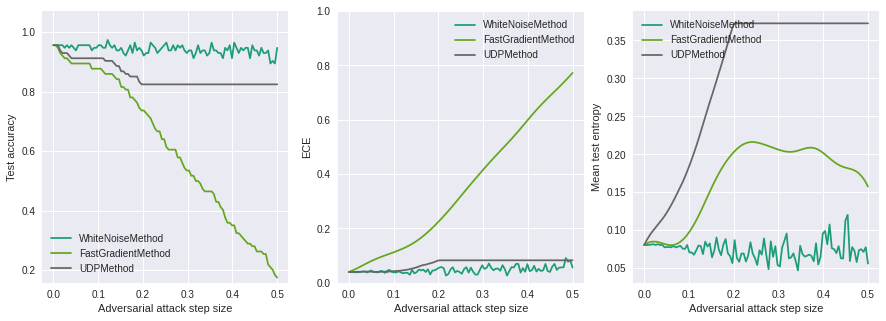
\includegraphics[width=\linewidth]{figures/eval/eval_adv_uq_train_fgsm.png}
      \caption{Adversarial training on the FGSM attack.}
    \end{subfigure}
     \begin{subfigure}{\textwidth}
      \centering
      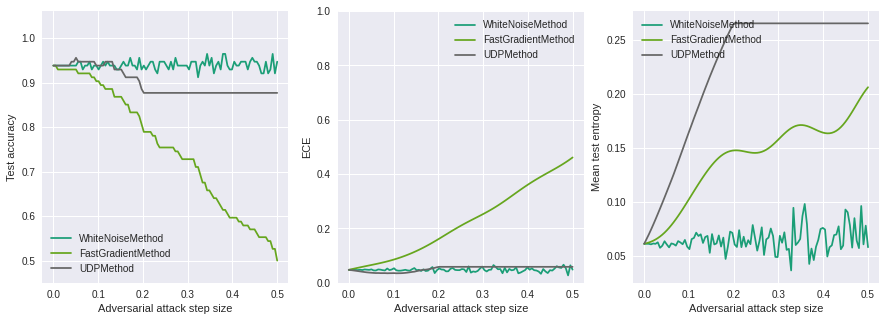
\includegraphics[width=\linewidth]{figures/eval/eval_adv_uq_train_udp.png}
      \caption{Adversarial training on the UDP attack.}
    \end{subfigure}
    \caption{Evaluation of an Adversarial Logistic Regression model (breast cancer dataset).}
    \label{fig:adversarial-evaluation-training}
\end{figure}

% adversarial ensembles 

\begin{figure}[!htbp]
    \begin{subfigure}{\textwidth}
      \centering
      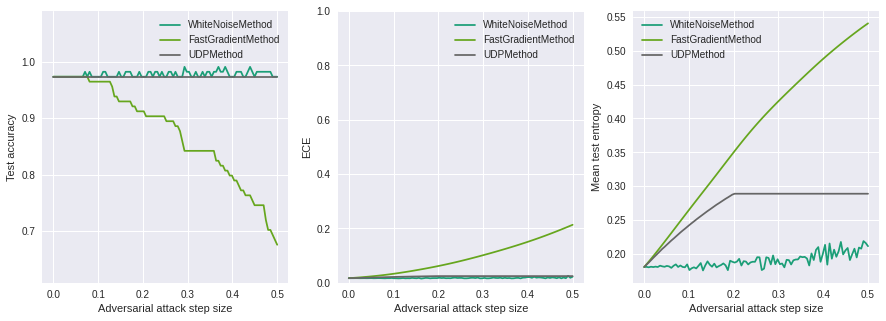
\includegraphics[width=\linewidth]{figures/eval/eval_adv_uq_train_ensemble_fgsm_mean.png}
     \caption{Evaluation on ensemble $mean$ attacks.}
    \end{subfigure}
    % \begin{subfigure}{\textwidth}
    %  \centering
    %  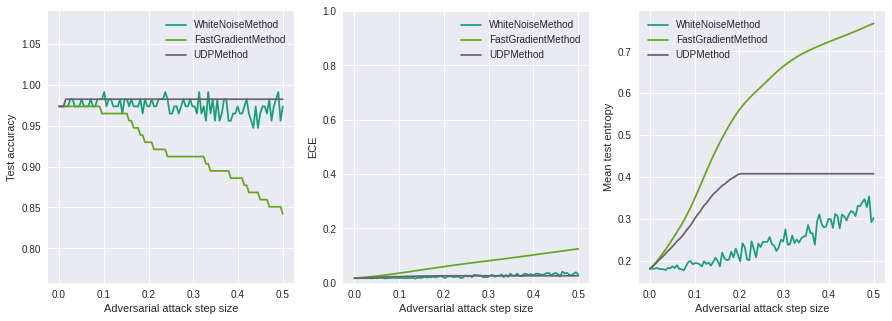
\includegraphics[width=\linewidth]{figures/eval/eval_adv_uq_train_ensemble_fgsm_first.png}
    %  \caption{Adversarial training on the ensemble first FGSM attack}
    %\end{subfigure}
     \begin{subfigure}{\textwidth}
      \centering
      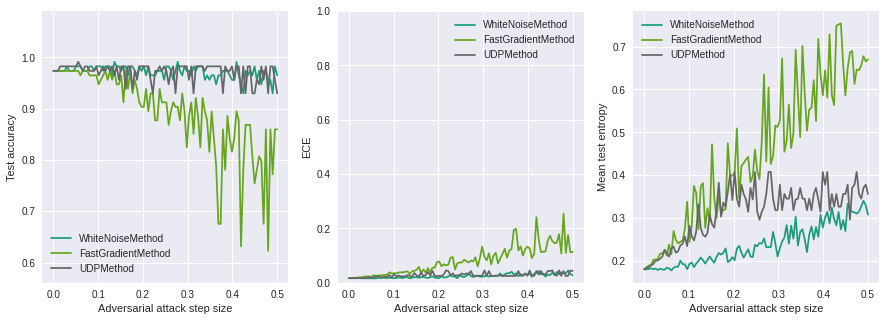
\includegraphics[width=\linewidth]{figures/eval/eval_adv_uq_train_ensemble_fgsm_random.png}
      \caption{Evaluation on ensemble $random$ attacks.}
    \end{subfigure}
    \begin{subfigure}{\textwidth}
      \centering
      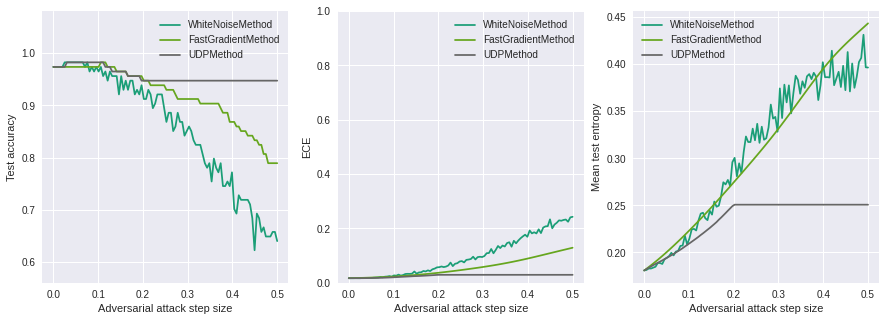
\includegraphics[width=\linewidth]{figures/eval/eval_adv_uq_train_ensemble_fgsm_max.png}
       \caption{Evaluation on ensemble $max$ attacks.}
    \end{subfigure}
    \caption{Evaluation of an Adversarial ensemble composed of 10 Logistic Regression models (breast cancer dataset). It is trained only on the FGSM attack.}
    \label{fig:adversarial-evaluation-training-ensemble-fgsm}
\end{figure}

This motivates the introduction of adversarial training (cf. algorithm \ref{alg:adversarial-training}) for uncertainty quantification to equip models with tools to handle OOD data points. The results of the adversarial training procedure of a Logistic Regression model are shown in figure \ref{fig:adversarial-evaluation-training}. Models are trained against one specific type of attack and evaluated on all attack types to assess generalisation. We observe that adversarial training on any attack improves the robustness of the model on all attacks: models are better calibrated and suffer less from overconfident incorrect predictions. In addition, robustness can be further improved by ensembling independently trained adversarial models. The latter models are evaluated on ensemble attacks aggregated using a $mean$, $random$ and $max$ aggregation function (cf. section \ref{section:design:adversarial} for more information about these attacks). Due to space constraints, only results on FGSM ensemble attacks are shared in this section. Still, the results can be generalised to other types of attacks, as shown in appendix \ref{appendix:adversarial-ensemble-plots}. From that experiment, we concluded that adversarial ensembles offer the strongest robustness against out-of-distribution data points. 


%- Evaluated 
%- Training an ensemble is also robust to different types of attacks (mean, first, %random, max).
%- Study how well training on a single perturbation influences the output.
%- Consider a single model: Logistic Regression. 


%\section{UQ in class imbalance settings}
% TODO


\section{Graph-to-text models}


\subsection{Evaluation of existing graph-to-text models} \label{experiment:G2T-raw-performance}
% exploration of hallucinations in both datasets
% report bleu scores of models
% observations: less hallucination of the predictions than reference text
\begin{table}[ht]
\centering
\caption{Performance of graph-to-text models on test set.}
\label{table:G2T-models}
\begin{tabular}[t]{lcclc} % p{3cm}
\toprule
Model & Bleu & Rouge & Faithfulness (fined-tuned NER) & Number faithfulness \\
\midrule
T5-base-WebNLG     & 0.632 & 0.744 & 0.996         & 0.972 \\
T5-small-WebNLG    & 0.626 & 0.740 & 0.995         & 0.966 \\
T5-base-SAR        & 0.511 & 0.588 & 0.763 (0.883) & 0.444 \\
T5-small-SAR       & 0.531 & 0.606 & 0.764 (0.876) & 0.473 \\
\bottomrule
\end{tabular}
\end{table}%

 The evaluation presented in this section is based on several T5 graph-to-text models trained on the WebNLG and SAR datasets. The performance of these models can be found in table \ref{table:G2T-models}. For the SAR dataset, faithfulness is evaluated using two different NER models: first, the base \textit{spaCy} model and, secondly, a fined-tuned model previously trained by a colleague at Oracle. More details about this NER model are available in appendix \ref{appendix:custom-ner-sar}.



In addition, table \ref{table:G2T-models-faithfulness} compares the hallucination ratio for model predictions and reference texts on the train and test sets. In contrast with the results of Dziri et al.\cite{originHalluDataOrModel}, the evaluation suggests that hallucinations are not amplified during testing compared to training. Furthermore, hallucinations appear slightly more frequently in the reference texts than in the actual model predictions. From a manual exploration of hallucinations occurring in the WebNLG and SAR datasets, a possible explanation could be human labelling errors in the reference texts that are not reproduced in the predictions. Some of them are highlighted in table \ref{table:G2T-models-errors}. Finally, the rather important number of hallucinations present in the SAR dataset (both reference texts and predictions) can be traced back to an issue in the data-gathering process. Indeed, several pieces of information available in the reference text cannot be found in the input graph (e.g. age of the persons of interest in the report). Hence, it is never possible for the model to produce a factual prediction for such elements. Additional edge types need to be included in the graph to mitigate this problem.

\begin{table}[!ht]
\centering
\caption{Comparison of hallucination ratios in graph-to-text models.}
\label{table:G2T-models-faithfulness}
\begin{tabular}[t]{lllcc} % p{3cm}
\toprule
 &  \multicolumn{2}{c}{$r_h$ (fined tuned NER)} & \multicolumn{2}{c}{$r_h^{num}$} \\
 \cmidrule(rl){2-3} \cmidrule(rl){4-5}
   Model  & train & test & train & test  \\
\midrule
Reference-WebNLG   & 0.016 & 0.011 & 0.039 & 0.040\\ 
T5-base-WebNLG     & 0.004 & 0.004 & 0.029 & 0.028\\
T5-small-WebNLG    & 0.007 & 0.005 & 0.034 & 0.034\\
Reference-SAR      & 0.254 (0.112) & 0.237 (0.107) & 0.561 & 0.582 \\ 
T5-base-SAR        & 0.254 (0.112) & 0.237 (0.117) & 0.564 & 0.556  \\
T5-small-SAR       & 0.253 (0.112) & 0.236 (0.124) & 0.562 & 0.527 \\
\bottomrule
\end{tabular}
\end{table}%


\begin{table}[!ht]
\centering
\caption{Examples of human labelling errors in WebNLG dataset.}
\label{table:G2T-models-errors}
\begin{tabular}[t]{cp{5cm}p{5cm}} % 
\toprule
Id & Graph edge & Reference text   \\
\midrule
0 & <H> 1097 Vicia <R> epoch is <T> \textbf{2006-12-31} & The epoch of 1097 Vicia is on \textbf{13 January 2016}. \\ 
1 & <H> Abradab <R> associated band/associated musical artist is <T> \textbf{Magik} (rapper) & He is with rapper associated with \textbf{Magri}. \\
\bottomrule
\end{tabular}
\end{table}%

\subsection{Relationship between entropy and hallucinations} \label{experiment:relation-entropy-hallucination}

This experiment aims to demonstrate whether or not a relationship between uncertainty and hallucination occurrence exists. Different UQ models lead to different uncertainty scores, impacting, in turn, hallucination detection performance. We provide insights into how the results are affected by the choice of UQ models. This experiment will also validate the introduction of the $MHE$ and $MHED$ metrics to evaluate UQ models.

To study the relationship between entropy and hallucination, the model $f$ is evaluated on both $D = \{(G_i, T_i)\}_i$ and the corresponding hallucination dataset $\Tilde{D} = \{(\Tilde{G_i}, T_i, a_i\}_i$. Given an input graph, i.e. $G_i$ or $\Tilde{G_i}$, the prediction entropy sequence is computed when the model is forced to re-generate the reference text $T_i$. Indeed, hallucination labels $a^i$ are paired up with the reference texts $T_i$ and are therefore useless if a brand new prediction $\hat T_i = f(G_i)$ is created. To force the model to re-generate $T_i$, the targeted decoding procedure defined in algorithm \ref{alg:targeted-decoding} is used. Let $\Entropy_i^D = \{ \Entropy_{i,j}^D \}_j = \{ \Entropy_{j}(G_i, T_i) \}_j$ be the entropy sequences generated using targeted decoding on dataset $D$. Let $\delta^D$ be the mean hallucination entropy difference (MHED) on dataset $D$ :

\begin{equation}
    MHED_i = \delta_i^D = \frac{\sum_j a_{i,j} \cdot \Entropy_{i,j}^D}{\sum_j a_{i,j}} - \frac{\sum_j \neg a_{i,j} \Entropy_{i,j}^D}{\sum_j \neg a_{i,j}}
\end{equation}


It allows us to compute the accepted hallucination noise level $\epsilon = \mu(\delta^D) = \frac{1}{N} \sum_n \delta^D_i $ since $D$ is not a hallucination dataset. This can be extended to the hallucination dataset $\Tilde{D}$ using the notation $\delta^{\Tilde{D}}_i$. The condition $s_i = I\{\delta^{\Tilde{D}}_i > \epsilon\}$ provides evidence that the model produced a higher entropy for hallucination tokens given the input graph $\Tilde{G_i}$. The robust condition $v_i =  I\left\{\delta^{\Tilde{D}}_i > \epsilon_{0.95}\right\}$ at 95\% confidence is also computed so that $\epsilon_{0.95} = \epsilon + 1.96 \frac{\sigma(\delta^D)}{\sqrt{N}}$.
% results
The results of this experiment are shared in table \ref{table:relationship-entropy-uncertainty}. The evaluation is performed on a truncated version of the test set where data points containing no hallucination have been dropped, e.g. $\{i \;:\; \forall_j \;a_{i,j} = 0\}$. We observe that the hallucination entropy difference on the hallucination dataset is significantly higher than on the non-hallucination one. This supports the claim that entropy is high for hallucination tokens compared to non-hallucinated ones. For the WebNLG dataset, $\mu(v) = 0.936$, i.e. for 93.6\% of the data points the claim holds. For the SAR dataset, the ratio is increased to 100\%. 


\begin{table}[ht]
\centering
\caption{Mean hallucination entropy difference for different test datasets. }
\label{table:relationship-entropy-uncertainty}
\begin{tabular}[t]{lcccccccc} % p{3cm}
\toprule
 & & \multicolumn{3}{c}{Dataset $D$} & \multicolumn{4}{c}{Hallucination dataset $\Tilde{D}$} \\
 \cmidrule(rl){3-5} \cmidrule(rl){6-9}
Model      &  $N$   & $\mu(\delta^D)$ & $\sigma(\delta^D)$ & $\epsilon_{0.95}$ & $\mu(\delta^{\Tilde{D}})$ & $\sigma(\delta^{\Tilde{D}})$ & $\mu(s)$ & $\mu(v)$  \\
\midrule
T5-base-WebNLG     & 530 & -0.30 & 0.50 & -0.23 & 1.16 & 0.95 & 0.943 & 0.936 \\
T5-base-SAR         & 21 & -0.02 & 0.07 & 0.01 & 0.20 & 0.11 & 1.000 & 1.000 \\
\bottomrule
\end{tabular}
\end{table}%

\subsection{Factual uncertainty evaluation of graph-to-text models}

In section \ref{experiment:relation-entropy-hallucination}, a relationship between uncertainty and hallucinations was established. It motivated the use of the factual uncertainty metrics introduced in section \ref{experiment:relation-entropy-hallucination} to evaluate the quality of UQ in a graph-to-text use case. Table \ref{table:UQ-G2T-models} contains the results of this evaluation for the mean hallucination entropy ($MHE$) and mean hallucination entropy difference ($MHED$) metrics. In addition, $MHED*$, a modified version of $MHED$, where all stop words and punctuation tokens have been dropped, is also reported.  

Predictions are generated using the targeted decoding (cf. algorithm \ref{alg:targeted-decoding}) to reproduce the reference texts of the test set. On both WebNLG and SAR datasets, the dropout ensemble outmatches the remaining ensemble models independently of the uncertainty type. Surprisingly, graph-encoding ensemble performs worse than a UQ model without an ensemble. This indicates that randomly shuffling the ordering of edges could negatively impact the performance of the graph-to-text generation process.
% report metrics of UQ models: calibration
% discuss MHED* metric
% targeted decoding to generate output

\begin{table}[!ht]
    \centering
        \caption{Factual performance of UQ graph-to-text models on test set.}
    \label{table:UQ-G2T-models}
     \centerline{
    \begin{tabular}{clccccccccc}
\toprule
& & \multicolumn{3}{c}{$MHE$} & \multicolumn{3}{c}{$MHED$} & \multicolumn{3}{c}{$MHED*$} \\
    \cmidrule(rl){3-5} \cmidrule(rl){6-8} \cmidrule(rl){9-11}
&Uncertainty &         data & model & total &         data & model & total &                           data & model & total \\
&Ensemble          &              &       &       &              &       &       &                                &       &       \\
\midrule
\multirow{3}{*}{\rotatebox{90}{WebNLG}}
& None           &  ---  &  ---  &	2.07 & 	--- & --- & 1.30  & --- 	&--- & 1.47 \\
& Graph encoding       &  1.82 &  0.01 &  1.84 &  1.28 &  0.01 &  1.29  &                       1.42 &  0.01 &  1.43  \\
& Deep           &  2.02 &  0.12 &  2.14 &  1.29 &  0.08 &  1.37  &                       1.45 &  0.09 &  1.54  \\
& Dropout        &  \textbf{2.15} &  \textbf{0.30} &  \textbf{2.45} &  \textbf{1.46} &  \textbf{0.23} &   \textbf{1.69} &                       \textbf{1.60} &  \textbf{0.24} &   \textbf{1.84} \\
% Dropout        &   \textbf{2.17 (0.1)} &  \textbf{0.30} &  \textbf{2.47} &  \textbf{1.46 (0.16)} &  0.22 &  \textbf{1.68} &                    \textbf{1.59 (0.12)} &  0.23 &  \textbf{1.82} \\
%&Encoding &  1.87 (-0.2) &  0.01 &  1.89 &  1.31 (0.01) &  0.01 &  1.32 &                   1.44 (-0.03) &  0.01 &  1.45 \\
%&Seed           &  2.13 (0.06) &  0.31 &  2.43 &  1.45 (0.15) &  \textbf{0.23} &  \textbf{1.68} &                    1.58 (0.11) &  \textbf{0.24} &  \textbf{1.82 }\\
\\
\multirow{3}{*}{\rotatebox{90}{SAR}}
& None           & ---	 &  ---  & 	0.86  & ---  & --- &	0.72 &	--- & --- & 0.70 \\
& Graph encoding       &  0.71 &  0.09 &   0.80 &  0.63 &  0.08 &  0.71  &                       0.63 &  0.08 &  0.70 \\
& Deep           &  0.74 &  0.41 &  1.15  &  0.62 &  0.35 &   0.97  &                       0.60 &  0.34 &  0.95 \\
& Dropout        &  \textbf{0.97} &  \textbf{0.49} &   \textbf{1.46} &  \textbf{0.83} &  \textbf{0.41} &   \textbf{1.24} &                       \textbf{0.82} &  \textbf{0.41} & \textbf{ 1.22} \\




%Dropout        &    0.4 (0.06) &  0.20 &  0.60 &   0.26 (0.05) &  0.12 &  0.38 &                0.25 (0.06) &  0.12 &  0.37 \\
%&Encoding &  0.25 (-0.09) &  0.03 &  0.28 &  0.17 (-0.04) &  0.02 &  0.19 &               0.17 (-0.02) &  0.02 &  0.18 \\
%&Seed           &    0.4 (0.06) &  0.20 &  0.59 &   0.26 (0.05) &  0.12 &  0.38 &                0.25 (0.06) &  0.12 &  0.37 \\


\bottomrule
\end{tabular}
}
\end{table}


\subsection{Entropy predictive power} \label{experiment:entropy-predictive-power}

The experiment of section \ref{experiment:relation-entropy-hallucination} has established the validity of the synthetic datasets as well as the relationship between uncertainty and hallucination occurrence. In this section, we formally evaluate the predictive power of entropy when it comes to token hallucination detection using the models defined in section \ref{design:hallucination-detection-models}:
\begin{itemize}
    \item Baseline hallucination detection based on NER. No model training or synthetic hallucination dataset is required with this approach.
    \item Logistic regression models based on different sets of features:
    \begin{itemize}
        \item Total uncertainty of the current token.
        \item Model and data uncertainty of the current token.
        \item Total uncertainty of the past five tokens (sequence model).
        \item Model and data uncertainty of the past five tokens (split uncertainty sequence model).
    \end{itemize}
\end{itemize}
The uncertainty of the model is compared across different model types: base, graph encoding, dropout, and a deep-seed ensemble, all of size 5. Word expansion (cf. section \ref{design:synthetic-hallucination-data}) is also applied to the best of these models as a post-processing step.

\begin{figure}[!ht]
    \centering
    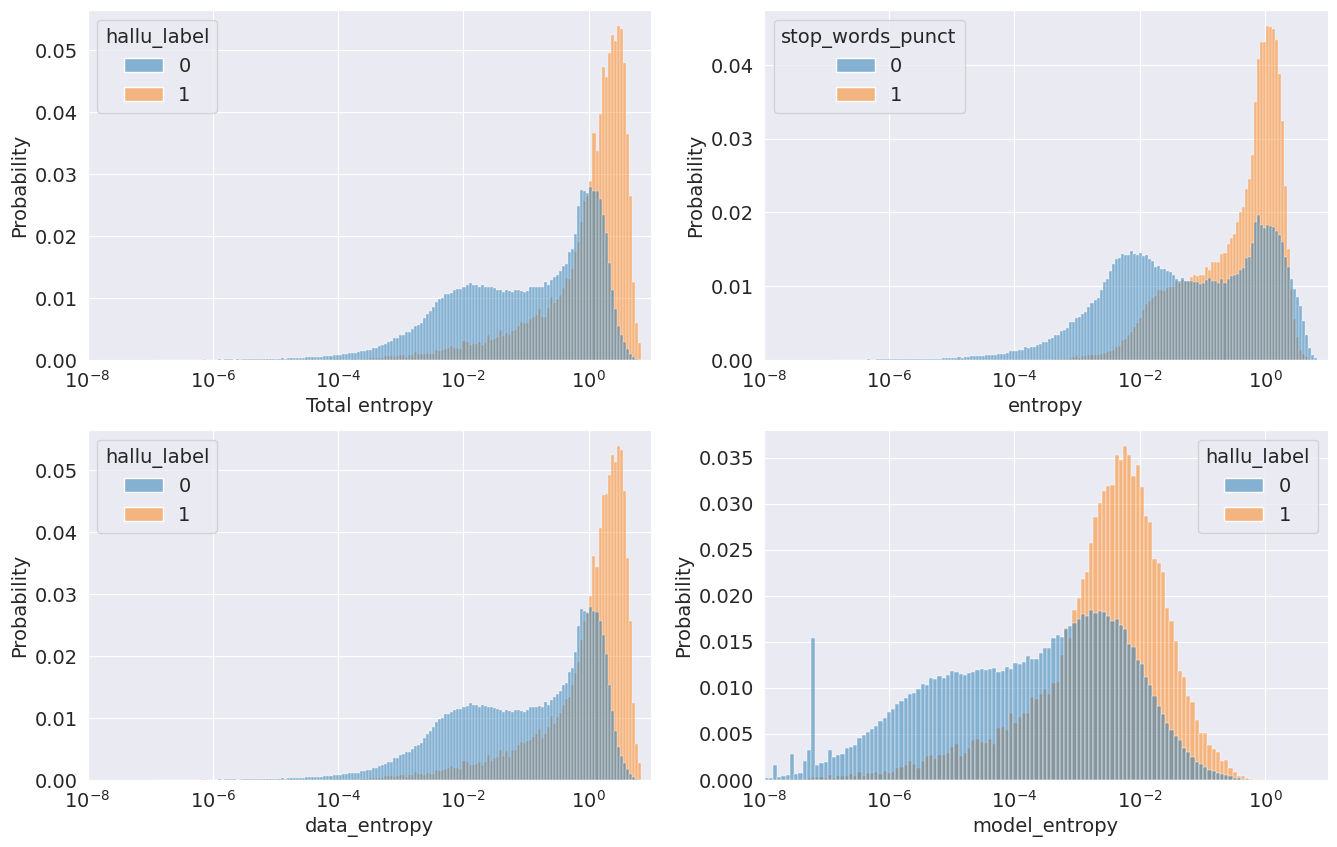
\includegraphics[width=0.85\linewidth]{figures/eval/entropy_pred_power/entropy_hist.png}
    \caption{Various histograms of token-level entropy (data, model and total) on the WebNLG dataset based computed using graph encoding ensembles.}
    \label{fig:entropy-hists}
\end{figure}

First, a simple data exploration step is carried out to visualise the entropy distribution for hallucination and non-hallucination tokens (cf. figure \ref{fig:entropy-hists}) based on the graph ensemble entropy predictions. The distributions of total entropy and data entropy are relatively similar, and a substantial probability mass can be witnessed for hallucination tokens with high entropies. This is less apparent for model entropy which could result in a smaller predictive power for this particular feature. In the top-right plot, the entropy distribution is also displayed for stop-words and punctuation tokens compared to other tokens. Intrinsically, stop-words and punctuation tokens do not meet the requirements to be considered hallucination or knowledge expression. However, the figure indicates significantly high entropies for these tokens. We decided to filter them out to improve the quality of the binary classification model. Given the spread of the x-axis in these plots, log and standard scaling preprocessing steps are applied to the entropy features. Similar conclusions can be drawn for the SAR dataset. 
% more on imbalance datasets



Besides, this classification task is strongly imbalanced, i.e. only 5.3\% of tokens are hallucination tokens for the WebNLG dataset and 1.6\% for the SAR dataset. The non-hallucination labels are also noisy. Indeed, some hallucinations are already present in the raw dataset, and they are not captured by the synthetic hallucination labels. Hence, false positives, e.g.  tokens that are not hallucinations but are predicted as such, are less critical than false negatives. Hence, recall is a more appropriate metric to consider than precision. When a strong imbalance is present, user-defined probability thresholds $T$, i.e. $\hat y_i = I\{p_{i,1} \geq T\}$, are commonly used to control better the number of acceptable false positives for each domain of applications.
For this reason, hallucination detection models are compared using Receiver Operating Characteristic (ROC) and Precision-Recall (PR) curves, for both datasets. Using the probabilistic interpretation of the $AUC-ROC$ metric, it can be shown that it is likely to be high for an imbalanced dataset. In contrast, $AUC-PC$ is better suited for such use cases and is the metric used to select the final model. 

\begin{figure}
     \centering
     \begin{subfigure}[b]{0.95\textwidth}
         \centering
         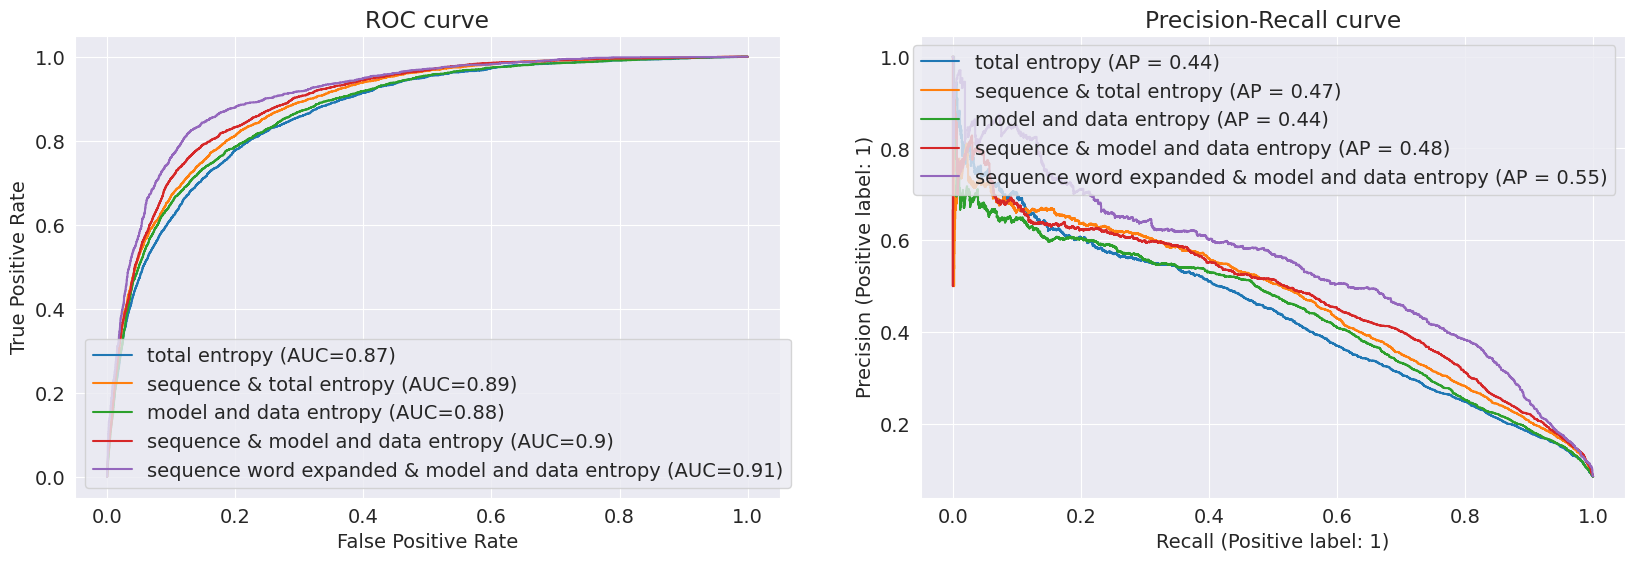
\includegraphics[width=\textwidth]{figures/eval/entropy_pred_power/WebNLG_dropout_ensemble.png}
         \caption{WebNLG dataset.}
         \label{fig:webnlg-local-ensemble-hallu-detection}
     \end{subfigure}
     \hfill
    \begin{subfigure}[b]{0.95\textwidth}
         \centering
         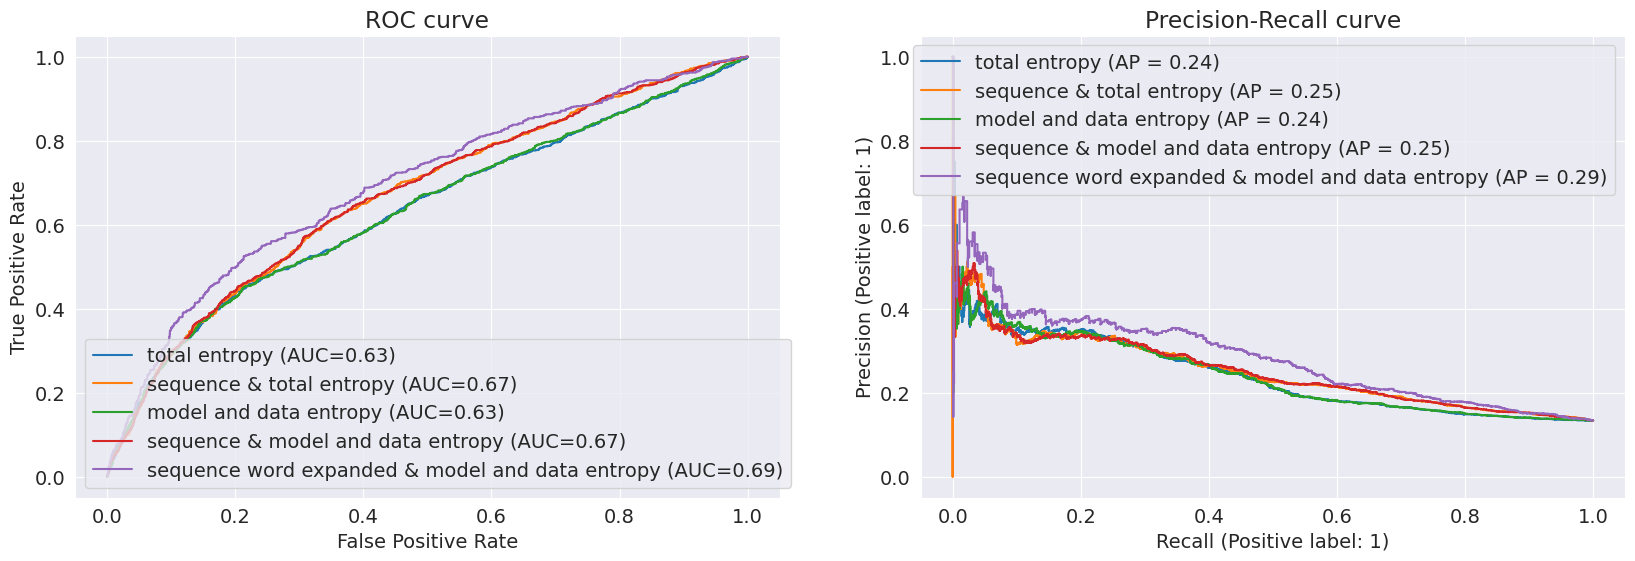
\includegraphics[width=\textwidth]{figures/eval/entropy_pred_power/SAR_hallu_dropout_results.png}
         \caption{SAR dataset.}
         \label{fig:sar-local-ensemble-hallu-detection}
     \end{subfigure}
     \hfill
     \hfill
       \caption{Comparison of Logistic regression models trained on various sets of features via $ROC$ and $PR$ curves. Entropies are generated using dropout ensemble}
        \label{fig:local-ensemble-hallu-detection}
\end{figure}
% table \ref{baseline-ner-hallucination-detection} contains 


In figure \ref{fig:local-ensemble-hallu-detection}, we observe that models achieving the best performance are those with the most extensive set of features, i.e. split uncertainty sequence models. The decomposition of total uncertainty into data and model components also leads to a slight improvement gap of around 0.01 in $AUC-PR$ for WebNLG but not SAR. Additionally, word expansion is a rather powerful tool as it increases the $AUC-PR$ score by 15\%. 

\begin{figure}[!ht]
     \centering
     \begin{subfigure}[b]{0.95\textwidth}
         \centering
         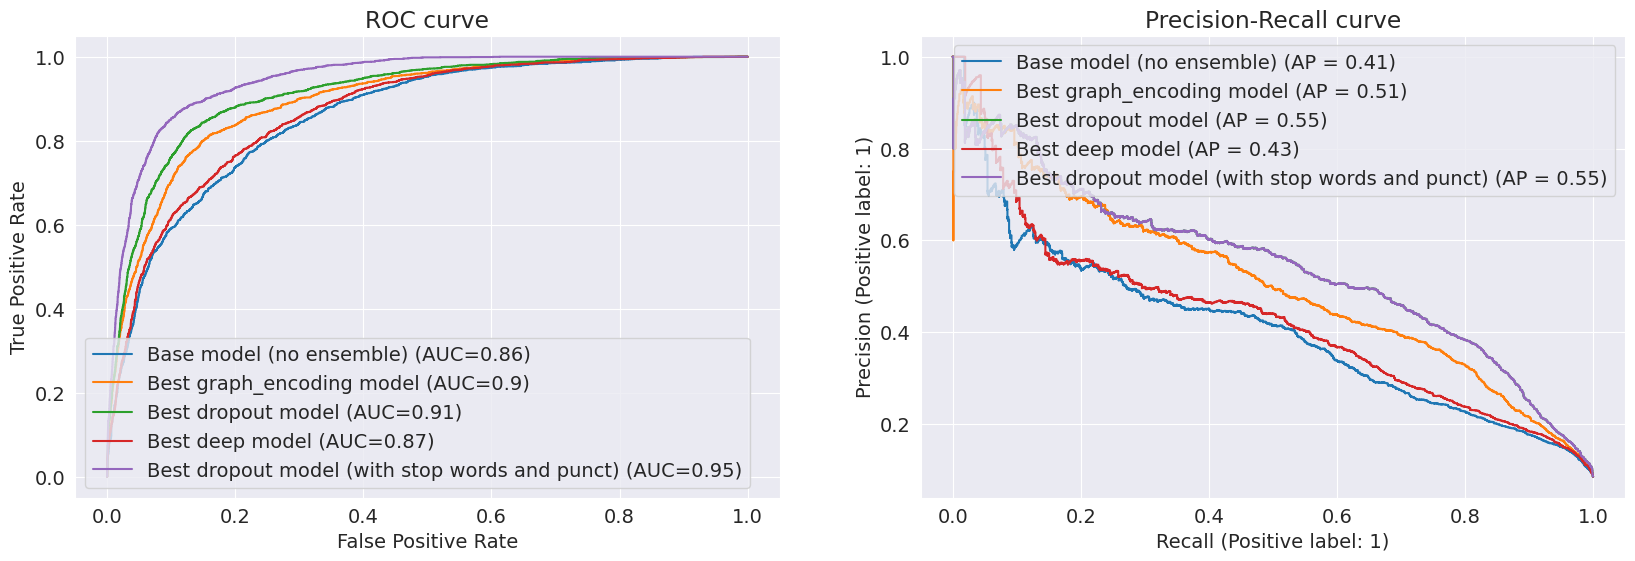
\includegraphics[width=\textwidth]{figures/eval/entropy_pred_power/webnlg_hd_results.png}
         \caption{WebNLG dataset.}
         \label{fig:webnlg-hallu-detection-best-results}
     \end{subfigure}
     \hfill
     \begin{subfigure}[b]{0.95\textwidth}
         \centering
         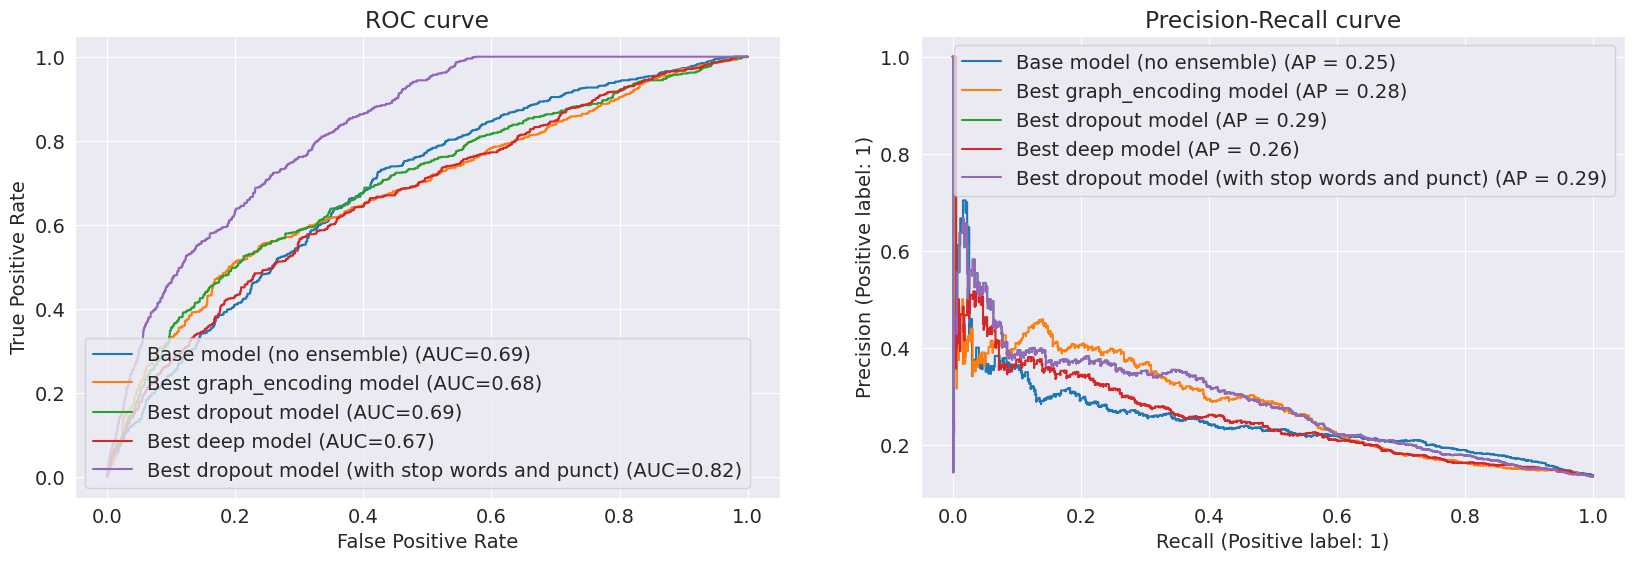
\includegraphics[width=\textwidth]{figures/eval/entropy_pred_power/SAR_hallu_results.png}
         \caption{SAR dataset.}
         \label{fig:sar-hallu-detection-best-results}
     \end{subfigure}
     \hfill
       \caption{Results of the entropy predictive power experiment. Split uncertainty sequence models generated by different ensemble UQ methods are compared.}
        \label{fig:experiment-hallu-detection}
\end{figure}

Figure \ref{fig:experiment-hallu-detection} extends this comparison to different ensembling techniques. Dropout ensembles obtain the best scores for both datasets. Surprisingly, deep seed ensembles do not reach their expected level of performance\cite{evalUQDatasetShift}. It would have been interesting to train these deep ensembles using more variations in the hyper-parameters and training schemes in the hope of bringing more variability in the output. However, given the time required to train and evaluate such models, as well as the time frame of this thesis, this is left as a future work step. Due to hallucinations present in the raw datasets, the precision of these models is not exceptionally high, as anticipated, especially for the SAR dataset. This can be explained by the larger hallucination ratio for the latter dataset (cf. \ref{table:G2T-models-faithfulness}).

Finally, table \ref{table:baseline-ner-hallucination-detection} summarises the performance of the best dropout ensemble models compared to baseline detection models based on named entity recognition. Entropy-based models generate better predictions than the baseline, which motivates further research to improve their quality.

\begin{table}[ht]
\centering
\caption{Comparison of NER and Ensemble-based hallucination detection models. Logistic regression predictions are generated using a threshold of $0.75$ for WebNLG and $0.40$ for SAR.}
\label{table:baseline-ner-hallucination-detection}
\begin{tabular}[t]{lcccccc} % p{3cm}
\toprule
& \multicolumn{3}{c}{Non-hallucination (label 0)} & \multicolumn{3}{c}{Hallucination (label 1)} \\
 \cmidrule(rl){2-4} \cmidrule(rl){5-7}
Model & precision & recall & f1-score & precision & recall & f1-score \\
\midrule
NER-baseline-WebNLG     &     0.93      & 0.91      & 0.92 &     0.17      & 0.21 & 0.19 \\
Dropout-ensembe-WebNLG & 0.99      &0.93   &   \textbf{0.96}  &     0.36    &  0.76   &   \textbf{0.48}  \\
NER-baseline-SAR        &      0.98    &  0.92   &  \textbf{ 0.95}   &  0.05      &0.21 &     0.08 \\
%0.87      & 0.91      & 0.89 &     0.21      & 0.16 & 0.18 \\
custom-NER-baseline-SAR &     1.00  &    0.83   &   0.91  &  0.10  &    0.94  &    0.18\\

Dropout-ensemble-SAR  & 0.95  &    0.93  &    0.94 &         0.34  &    0.39  &    \textbf{0.37} \\

%&  0.99  &    0.93  &    0.96   &     0.39  &    0.79 &     0.52\\

\bottomrule
\end{tabular}
\end{table}%



Examples of the binary predictions of the hallucination detection models are shown below for the WebNLG dataset. Hallucination ground truth labels are \textit{"Denmark"} and \textit{"Universitas Aarhusiensis"}. Using a rather conservative threshold of $0.75$, the following prediction is constructed:


\epigraph{
The School of Business and Social Sciences at the Aarhus University is located in Aarhus, Denmark, and it was established in 1928. Its dean is Thomas Pallesen, and it has 16,000 students. Its Latin name is "\textcolor{BrickRed}{\textbf{Universitas Aarhusiensis}}". It is affiliated to the European University Association.
}{Dropout ensemble prediction with probability threshold $0.75$}

At token-level, the precision is 1.00, and the recall is 0.9. However, even if the graph does not contain an edge about Denmark, one might argue that the language model could infer that information from the city of Aarhus. By setting a lower value threshold, e.g. 0.5, recall improves to $1.00$ to the detriment of precision which goes down to $0.59$:

\epigraph{
The School of Business and Social Sciences at the Aarhus University is located in \textcolor{BrickRed}{\textbf{Aarhus, Denmark}}, and it was established in 1928. Its \textcolor{BrickRed}{\textbf{dean}} is Thomas Pallesen, and it has 16,000 students. Its \textcolor{BrickRed}{\textbf{Latin}} name is "\textcolor{BrickRed}{\textbf{Universitas Aarhusiensis}}". It is \textcolor{BrickRed}{\textbf{affiliated}} to the European University Association.
}{Dropout ensemble prediction with probability threshold $0.50$} 


%%%%%%%%%%%%%%%%%%%%
\chapter{Conclusion}
%%%%%%%%%%%%%%%%%%%%



%In the conclusion, you repeat the main result and finalise the discussion of
%your project. Mention the core results and why and how your system
%advances the status quo.

\section{Contributions}

In this thesis, I developed an uncertainty quantification package that can transform any \textit{scikit-learn} compatible estimator into an estimator capable of evaluating its uncertainty. It gathers models from the scientific literature and existing open-source libraries such as \textit{scikit-learn}, \textit{CatBoost} and \textit{XGBoost} in a standardised and user-friendly API. Models can be trained and evaluated, and predictions can be visualised using pre-defined plots. Additionally, the adversarial training capabilities provide UQ robustness to out-of-distribution data.

Due to the package's versatility, it can be applied to a vast range of applications. Existing non-UQ machine learning workflows can effortlessly leverage the package's capabilities by simply using one of our wrappers. No expertise in UQ is required to start experimenting with it, which fosters its adoption.  

% recalibration tools
% Results can be generalised to other types of attacks.
This package has been validated on the Boston housing and breast cancer datasets. Ensembles of Random Forests and Gradient Boosted Trees generally lead to the top UQ performance in our experiments. For models such as RF or GBT, intrinsic UQ seems to yield better results than an extrinsic model based on quantile regression. However, these results should be cautiously considered, as they are dataset dependent. 
When it comes to out-of-distribution UQ robustness, models were evaluated using three different types of attacks. It was shown that adversarial training based on any of these attacks improves UQ quality, which is generalisable to all attack types considered in this work. Furthermore, adversarial ensembles were introduced to enhance the performance even further.   
% Models trained to defend against a single attack demonstrate generalisation properties to others.
\newpage 


In the field of factuality for graph-to-text models, a relationship between entropy and hallucination has been established via an evaluation process on a synthetic dataset. The latter was focused on hallucinations occurring due to missing edge information and was built specifically for this purpose. This development motivated the introduction of two factual UQ metrics: the mean hallucination entropy and mean hallucination entropy difference. In addition, the binary labels delivered by the synthetic dataset enabled us to experiment with hallucination detection models. Logistic Regression models were trained based on different variations of entropy features. Due to hallucinations in the raw dataset, the false synthetic labels are noisy, hurting the model's precision. Nevertheless, dropout ensembles outperformed the remaining models and the NER baseline with a score of 0.55 in terms of $AUC-PR$. Given the imbalance of the dataset, it translates into a decent detection model. 


\section{Future work}
% deep ensemble might be overfitting
The work accomplished in this thesis naturally suffers from some limitations. They are discussed in the following sections, along with areas for improvement.

%of the framework

\subsection{Adversarial robustness}

Further investigations in the field of adversarial UQ robustness are essential to fortify our models against unexpected challenges and increase trust in their predictions, especially in real-world situations where the stakes are high.

The current evaluation was only performed using three attacks for the Logistic Regression model due to the limitations of the \textit{ART} library. Indeed, \textit{ART} is image-oriented and only offers a limited set of attacks for tabular data. Some experimentation has been carried out with two other attacks: Hop Skip Jump\cite{HopSkipJump} and Targeted Universal Perturbations\cite{TargetedUniversalPerturbations}. However, modifying their attack step size is impossible, which does not fit well with our evaluation setup. Regarding models,  Logistic Regression and C-Support Vector classification are the only supported \textit{scikit-learn} models that can be attacked by FGSM. Consequently, additional research to support more attacks on tabular data and models to extend the \textit{ART} library and evaluation framework would be a suitable subsequent step.

Besides, a qualitative assessment of the plots is required to evaluate the models. The package would benefit from the creation and validation of a formal metric for out-of-distribution UQ evaluation. For instance, given an ordered attack step size series $\{\epsilon_i\}_i$ and the corresponding series of mean entropies $\Bar{\Entropy} = \{\Bar{\Entropy_i}(\epsilon_i)\}_i$, a candidate metric could be the area between $\Bar{\Entropy}$ and its cumulative maximum series.

\subsection{UQ for graph-to-text}

First of all, table \ref{table:G2T-models} suggests that an improvement in the quality of the graph-to-text model, e.g. in BLEU score, correlates with an improvement in the faithfulness of the model and impacts UQ performance. In that regard, we could not reach the same $T5$ performance level as reported in the JointGT\cite{JointGT} paper, which could have affected the results. There is a difference of 0.0122 in BLEU score.

The only source of hallucination covered in this work concerns missing edge information. However, other important sources should not be neglected, e.g. human labelling errors or the misrepresentation of numbers as tokens\cite{surveyHallucination, representingNumbersNLP}. Given the importance of numbers in financial applications, it would be interesting to reflect on developing a specialised UQ tool for dealing with them.

The performance issues with the graph-encoding ensembles are also an area that could be further investigated. For instance, we tried to train graph-to-text models with data augmentation based on multiple graph linearisations. However, the reported performance was inferior to the base model. Specialised linearisations constructed using BFS or DFS traversals could bring an improvement compared to random ones. Deep-seed ensembles were also expected to perform better. As stated in section \ref{experiment:entropy-predictive-power}, training hyper-parameter ensembles to bring more variability in the output is a promising direction to look at.

If the hallucination detection models of section \ref{design:hallucination-detection-models} were primarily introduced to study the predictive power of entropy for this task, some research for extra features to be added to the model is probably required to be able to use it in production. An orthogonal research direction could be to rephrase the detection task as a named entity recognition task with a single label. Hence, transformers-based architecture could be used with updated embedding layers to incorporate entropy features.

Finally, the UQ evaluation was carried out using the targeted decoding procedure (cf. algorithm \ref{alg:targeted-decoding}) to reproduce the reference texts. However, a more realistic approach would be to rely on the texts generated by the graph-to-text model. The hallucination detection model of section \ref{experiment:entropy-predictive-power} could be applied to the test set to generate the prediction labels $\{\hat{a}_{i,j}\}_{i,j}$ and, therefore, compute the $MHE$ value. It introduces some flexibility regarding the choice of decoding algorithm, and a study of their impact on UQ quality could also be conducted.  

 
%Recently, variations of decoding and sampling algorithms have been introduced.
%Use conformal prediction to select a proper $p$ in decoding to produce calibrated outputs.

%Transform ensembling can also be performed using different techniques than targeted decoding.


\cleardoublepage
\phantomsection
\addcontentsline{toc}{chapter}{Bibliography}
\printbibliography


\appendix

\chapter{Adversarial ensemble evaluation} \label{appendix:adversarial-ensemble-plots}

This appendix is an extension of the out-of-distribution evaluation experiment of section \ref{experiment:OOD-evaluation}. The evaluation of adversarial ensembles trained on white noise attack is shared in figure \ref{fig:adversarial-evaluation-training-ensemble-noise}. Figure \ref{fig:adversarial-evaluation-training-ensemble-udp} contains the equivalent results for the UDP attack. As stated in section \ref{experiment:OOD-evaluation}, robustness is assessed via ensemble attacks aggregated using the $mean$, $random$ and $max$ functions.

\begin{figure}[htbp]
    \begin{subfigure}{\textwidth}
      \centering
      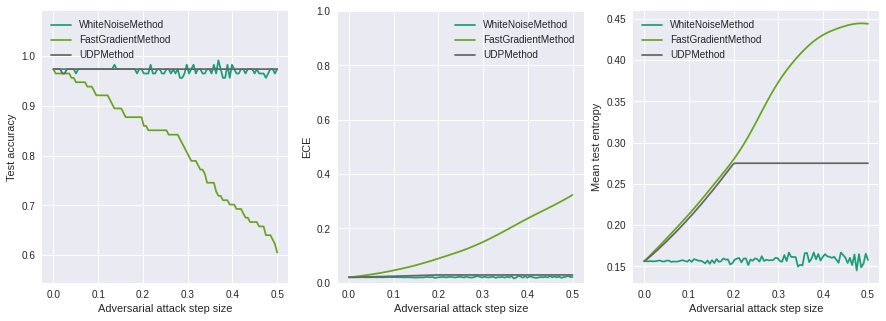
\includegraphics[width=\linewidth]{figures/eval/eval_adv_uq_train_ensemble_noise_mean.png}
      \caption{Evaluation on ensemble $mean$ attacks.}
    \end{subfigure}
    % \begin{subfigure}{\textwidth}
    %  \centering
    %  \includegraphics[width=\linewidth]{figures/eval/eval_adv_uq_train_ensemble_fgsm_first.png}
    %  \caption{Adversarial training on the ensemble first FGSM attack}
    %\end{subfigure}
     \begin{subfigure}{\textwidth}
      \centering
      \includegraphics[width=\linewidth]{figures/eval/eval_adv_uq_train_ensemble_noise_random.png}
      \caption{Evaluation on ensemble $random$ attacks.}
    \end{subfigure}
    \begin{subfigure}{\textwidth}
      \centering
      \includegraphics[width=\linewidth]{figures/eval/eval_adv_uq_train_ensemble_noise_max.png}
      \caption{Evaluation on ensemble $max$ attacks.}
    \end{subfigure}
    \caption{Evaluation of an Adversarial ensemble composed of 10 Logistic Regression models (breast cancer dataset). It is trained only on the white noise attack.}
    \label{fig:adversarial-evaluation-training-ensemble-noise}
\end{figure}

\begin{figure}[htbp]
    \begin{subfigure}{\textwidth}
      \centering
      \includegraphics[width=\linewidth]{figures/eval/eval_adv_uq_train_ensemble_udp_mean.png}
       \caption{Evaluation on ensemble $mean$ attacks.}
    \end{subfigure}
    % \begin{subfigure}{\textwidth}
    %  \centering
    %  \includegraphics[width=\linewidth]{figures/eval/eval_adv_uq_train_ensemble_fgsm_first.png}
    %  \caption{Adversarial training on the ensemble first FGSM attack}
    %\end{subfigure}
     \begin{subfigure}{\textwidth}
      \centering
      \includegraphics[width=\linewidth]{figures/eval/eval_adv_uq_train_ensemble_udp_random.png}
       \caption{Evaluation on ensemble $random$ attacks.}
    \end{subfigure}
    \begin{subfigure}{\textwidth}
      \centering
      \includegraphics[width=\linewidth]{figures/eval/eval_adv_uq_train_ensemble_udp_max.png}
      \caption{Evaluation on ensemble $max$ attacks.}
    \end{subfigure}
    \caption{Evaluation of an Adversarial ensemble composed of 10 Logistic Regression models (breast cancer dataset). It is trained only on the UDP attack.}
    \label{fig:adversarial-evaluation-training-ensemble-udp}
\end{figure}


\chapter{Named Entity Recognition fine-tuned on the SAR dataset} \label{appendix:custom-ner-sar}

In section \ref{experiment:G2T-raw-performance}, the performance and faithfulness of the graph-to-text models are evaluated. For the SAR dataset, a custom, fined-tuned NER model is mentioned. This section provides some information about the latter. 


The model is based on the RoBERTa transformer architecture and fine-tuned using the spaCy library. It was introduced in 2022 by D. Tekin, a colleague at Oracle, for his work on 
Knowledge Graph Construction from Unstructured Text using Named Entity Recognition, Relation Extraction, and Coreference Resolution. The performance of his approach is reported in table \ref{tab:NER-doga-performance} for the CoNLL-2004\cite{CoNLL4},  SciERC\cite{SciERC} and SAR datasets for comparison purposes.


\begin{table}[!ht]
    \centering
    \begin{tabular}{llcc}
    \toprule
        Dataset        & Model      & Micro-F1 & Macro-F1  \\
    \midrule
        CoNLL-2004     & Wang and Lu.,2020\cite{Lu2020} & 90.10 & 86.90 \\
        CoNLL-2004     & Tekin, 2022 & 90.34 & 87.19 \\
        SciERC         &  Luan et al.\cite{SciERC}, 2018 & 64.20 & --- \\
        SciERC         & Tekin, 2022 & 66.80 & --- \\
        SAR            & Tekin, 2022 & 88.82 & --- \\             
         \bottomrule
    \end{tabular}
    \caption{Performance of various NER models.}
    \label{tab:NER-doga-performance}
\end{table}



% Appendices are optional
% \appendix
% %%%%%%%%%%%%%%%%%%%%%%%%%%%%%%%%%%%%%%
% \chapter{How to make a transmogrifier}
% %%%%%%%%%%%%%%%%%%%%%%%%%%%%%%%%%%%%%%
%
% In case you ever need an (optional) appendix.
%
% You need the following items:
% \begin{itemize}
% \item A box
% \item Crayons
% \item A self-aware 5-year old
% \end{itemize}

\end{document}